\documentclass[twoside]{book}

% Packages required by doxygen
\usepackage{calc}
\usepackage{doxygen}
\usepackage{graphicx}
\usepackage[utf8]{inputenc}
\usepackage{makeidx}
\usepackage{multicol}
\usepackage{multirow}
\usepackage{textcomp}
\usepackage[table]{xcolor}

% Font selection
\usepackage[T1]{fontenc}
\usepackage{mathptmx}
\usepackage[scaled=.90]{helvet}
\usepackage{courier}
\usepackage{amssymb}
\usepackage{sectsty}
\renewcommand{\familydefault}{\sfdefault}
\allsectionsfont{%
  \fontseries{bc}\selectfont%
  \color{darkgray}%
}
\renewcommand{\DoxyLabelFont}{%
  \fontseries{bc}\selectfont%
  \color{darkgray}%
}

% Page & text layout
\usepackage{geometry}
\geometry{%
  a4paper,%
  top=2.5cm,%
  bottom=2.5cm,%
  left=2.5cm,%
  right=2.5cm%
}
\tolerance=750
\hfuzz=15pt
\hbadness=750
\setlength{\emergencystretch}{15pt}
\setlength{\parindent}{0cm}
\setlength{\parskip}{0.2cm}
\makeatletter
\renewcommand{\paragraph}{%
  \@startsection{paragraph}{4}{0ex}{-1.0ex}{1.0ex}{%
    \normalfont\normalsize\bfseries\SS@parafont%
  }%
}
\renewcommand{\subparagraph}{%
  \@startsection{subparagraph}{5}{0ex}{-1.0ex}{1.0ex}{%
    \normalfont\normalsize\bfseries\SS@subparafont%
  }%
}
\makeatother

% Headers & footers
\usepackage{fancyhdr}
\pagestyle{fancyplain}
\fancyhead[LE]{\fancyplain{}{\bfseries\thepage}}
\fancyhead[CE]{\fancyplain{}{}}
\fancyhead[RE]{\fancyplain{}{\bfseries\leftmark}}
\fancyhead[LO]{\fancyplain{}{\bfseries\rightmark}}
\fancyhead[CO]{\fancyplain{}{}}
\fancyhead[RO]{\fancyplain{}{\bfseries\thepage}}
\fancyfoot[LE]{\fancyplain{}{}}
\fancyfoot[CE]{\fancyplain{}{}}
\fancyfoot[RE]{\fancyplain{}{\bfseries\scriptsize Generated on Fri Aug 29 2014 17\-:01\-:18 for S\-E306 Project 1 by Doxygen }}
\fancyfoot[LO]{\fancyplain{}{\bfseries\scriptsize Generated on Fri Aug 29 2014 17\-:01\-:18 for S\-E306 Project 1 by Doxygen }}
\fancyfoot[CO]{\fancyplain{}{}}
\fancyfoot[RO]{\fancyplain{}{}}
\renewcommand{\footrulewidth}{0.4pt}
\renewcommand{\chaptermark}[1]{%
  \markboth{#1}{}%
}
\renewcommand{\sectionmark}[1]{%
  \markright{\thesection\ #1}%
}

% Indices & bibliography
\usepackage{natbib}
\usepackage[titles]{tocloft}
\setcounter{tocdepth}{3}
\setcounter{secnumdepth}{5}
\makeindex

% Hyperlinks (required, but should be loaded last)
\usepackage{ifpdf}
\ifpdf
  \usepackage[pdftex,pagebackref=true]{hyperref}
\else
  \usepackage[ps2pdf,pagebackref=true]{hyperref}
\fi
\hypersetup{%
  colorlinks=true,%
  linkcolor=blue,%
  citecolor=blue,%
  unicode%
}

% Custom commands
\newcommand{\clearemptydoublepage}{%
  \newpage{\pagestyle{empty}\cleardoublepage}%
}


%===== C O N T E N T S =====

\begin{document}

% Titlepage & ToC
\hypersetup{pageanchor=false}
\pagenumbering{roman}
\begin{titlepage}
\vspace*{7cm}
\begin{center}%
{\Large S\-E306 Project 1 }\\
\vspace*{1cm}
{\large Generated by Doxygen 1.8.6}\\
\vspace*{0.5cm}
{\small Fri Aug 29 2014 17:01:18}\\
\end{center}
\end{titlepage}
\clearemptydoublepage
\tableofcontents
\clearemptydoublepage
\pagenumbering{arabic}
\hypersetup{pageanchor=true}

%--- Begin generated contents ---
\chapter{Softeng 306 Project 1}
\label{index}\hypertarget{index}{}

{\bfseries se306\-\_\-project1} 

--$>$ 
\chapter{Software Engineering Design 2 Group 6}
\label{md_Documentation_README}
\hypertarget{md_Documentation_README}{}
\paragraph*{Department of Electrical and Computer Engineering, University of Auckland}

\subsection*{Project 1\-: Group robotic behavior simulation using Robot Operating System (R\-O\-S)}

\subsubsection*{Table of Contents}


\begin{DoxyItemize}
\item \href{#about}{\tt R\-O\-S Project}
\item \href{#team-members}{\tt Team Members}
\end{DoxyItemize}

\subsection*{\label{_about}%
R\-O\-S Project}

In this project, we simulate small groups of robots that show simple collective behaviours, as explored in Swarm Robotics. The robots achieve collective behaviour through message exchanges. This is simulated in a graphical simulator.

\subsection*{\label{_team-members}%
Team Members}

{\bfseries Samanyu Kansara}\par
 Project Lead\par
\par
 {\bfseries John Lee}\par
 Solutions Architect\par
\par
 {\bfseries Harriet Robinson-\/\-Chen}\par
 Systems Analyst, Documentalist\par
\par
 {\bfseries Alan Lau}\par
 Planner, Systems Analyst\par
\par
 {\bfseries Mustafa Shehadeh}\par
 Software Designer\par
\par
 {\bfseries Dae Kyung Kim}\par
 Software Designer\par
\par
 {\bfseries Kester Balmes}\par
 Quality Engineer, Tester\par
\par
 {\bfseries Rodel Jasper Rojos}\par
 Quality Engineer, Tester\par
\par
 {\bfseries Govindalf Von Samarasinghe}\par
 Installer, Configuration Manager\par
\par
 
\chapter{Software Engineering Design 2 Group 6}
\label{md_README}
\hypertarget{md_README}{}
\paragraph*{Department of Electrical and Computer Engineering, University of Auckland}

\subsection*{Project 1\-: Group robotic behavior simulation using Robot Operating System (R\-O\-S)}

\subsubsection*{Table of Contents}


\begin{DoxyItemize}
\item \href{#about}{\tt R\-O\-S Project}
\item \href{#team-members}{\tt Team Members}
\end{DoxyItemize}

\subsection*{\label{_about}%
R\-O\-S Project}

In this project, we simulate small groups of robots that show simple collective behaviours, as explored in Swarm Robotics. The robots achieve collective behaviour through message exchanges. This is simulated in a graphical simulator.

\subsection*{\label{_team-members}%
Team Members}

{\bfseries Samanyu Kansara}\par
 Project Lead\par
\par
 {\bfseries John Lee}\par
 Solutions Architect\par
\par
 {\bfseries Harriet Robinson-\/\-Chen}\par
 Systems Analyst, Documentalist\par
\par
 {\bfseries Alan Lau}\par
 Planner, Systems Analyst\par
\par
 {\bfseries Mustafa Shehadeh}\par
 Software Designer\par
\par
 {\bfseries Dae Kyung Kim}\par
 Software Designer\par
\par
 {\bfseries Kester Balmes}\par
 Quality Engineer, Tester\par
\par
 {\bfseries Rodel Jasper Rojos}\par
 Quality Engineer, Tester\par
\par
 {\bfseries Govindalf Von Samarasinghe}\par
 Installer, Configuration Manager\par
\par
 
\chapter{Namespace Index}
\section{Namespace List}
Here is a list of all documented namespaces with brief descriptions\-:\begin{DoxyCompactList}
\item\contentsline{section}{\hyperlink{namespaceAgentConst}{Agent\-Const} \\*Enum representing the different types of agent }{\pageref{namespaceAgentConst}}{}
\item\contentsline{section}{\hyperlink{namespacese306__project1_1_1msg_1_1__AssistantMsg}{se306\-\_\-project1.\-msg.\-\_\-\-Assistant\-Msg} }{\pageref{namespacese306__project1_1_1msg_1_1__AssistantMsg}}{}
\item\contentsline{section}{\hyperlink{namespacese306__project1_1_1msg_1_1__DoctorMsg}{se306\-\_\-project1.\-msg.\-\_\-\-Doctor\-Msg} }{\pageref{namespacese306__project1_1_1msg_1_1__DoctorMsg}}{}
\item\contentsline{section}{\hyperlink{namespacese306__project1_1_1msg_1_1__ResidentMsg}{se306\-\_\-project1.\-msg.\-\_\-\-Resident\-Msg} }{\pageref{namespacese306__project1_1_1msg_1_1__ResidentMsg}}{}
\end{DoxyCompactList}

\chapter{Hierarchical Index}
\section{Class Hierarchy}
This inheritance list is sorted roughly, but not completely, alphabetically\-:\begin{DoxyCompactList}
\item \contentsline{section}{Agent}{\pageref{classAgent}}{}
\begin{DoxyCompactList}
\item \contentsline{section}{Assistant}{\pageref{classAssistant}}{}
\item \contentsline{section}{Resident}{\pageref{classResident}}{}
\item \contentsline{section}{Visitor}{\pageref{classVisitor}}{}
\begin{DoxyCompactList}
\item \contentsline{section}{Caregiver}{\pageref{classCaregiver}}{}
\item \contentsline{section}{Doctor}{\pageref{classDoctor}}{}
\item \contentsline{section}{Friend}{\pageref{classFriend}}{}
\item \contentsline{section}{Nurse}{\pageref{classNurse}}{}
\item \contentsline{section}{Relative}{\pageref{classRelative}}{}
\end{DoxyCompactList}
\end{DoxyCompactList}
\item \contentsline{section}{Agent\-Factory}{\pageref{classAgentFactory}}{}
\item \contentsline{section}{se306\-\_\-project1\-:\-:Assistant\-Msg\-\_\-$<$ Container\-Allocator $>$}{\pageref{structse306__project1_1_1AssistantMsg__}}{}
\item \contentsline{section}{ros\-:\-:message\-\_\-traits\-:\-:Data\-Type$<$ \-:\-:se306\-\_\-project1\-:\-:Assistant\-Msg\-\_\-$<$ Container\-Allocator $>$ $>$}{\pageref{structros_1_1message__traits_1_1DataType_3_01_1_1se306__project1_1_1AssistantMsg___3_01ContainerAllocator_01_4_01_4}}{}
\item \contentsline{section}{ros\-:\-:message\-\_\-traits\-:\-:Data\-Type$<$ \-:\-:se306\-\_\-project1\-:\-:Doctor\-Msg\-\_\-$<$ Container\-Allocator $>$ $>$}{\pageref{structros_1_1message__traits_1_1DataType_3_01_1_1se306__project1_1_1DoctorMsg___3_01ContainerAllocator_01_4_01_4}}{}
\item \contentsline{section}{ros\-:\-:message\-\_\-traits\-:\-:Data\-Type$<$ \-:\-:se306\-\_\-project1\-:\-:Resident\-Msg\-\_\-$<$ Container\-Allocator $>$ $>$}{\pageref{structros_1_1message__traits_1_1DataType_3_01_1_1se306__project1_1_1ResidentMsg___3_01ContainerAllocator_01_4_01_4}}{}
\item \contentsline{section}{ros\-:\-:message\-\_\-traits\-:\-:Definition$<$ \-:\-:se306\-\_\-project1\-:\-:Assistant\-Msg\-\_\-$<$ Container\-Allocator $>$ $>$}{\pageref{structros_1_1message__traits_1_1Definition_3_01_1_1se306__project1_1_1AssistantMsg___3_01ContainerAllocator_01_4_01_4}}{}
\item \contentsline{section}{ros\-:\-:message\-\_\-traits\-:\-:Definition$<$ \-:\-:se306\-\_\-project1\-:\-:Doctor\-Msg\-\_\-$<$ Container\-Allocator $>$ $>$}{\pageref{structros_1_1message__traits_1_1Definition_3_01_1_1se306__project1_1_1DoctorMsg___3_01ContainerAllocator_01_4_01_4}}{}
\item \contentsline{section}{ros\-:\-:message\-\_\-traits\-:\-:Definition$<$ \-:\-:se306\-\_\-project1\-:\-:Resident\-Msg\-\_\-$<$ Container\-Allocator $>$ $>$}{\pageref{structros_1_1message__traits_1_1Definition_3_01_1_1se306__project1_1_1ResidentMsg___3_01ContainerAllocator_01_4_01_4}}{}
\item \contentsline{section}{se306\-\_\-project1\-:\-:Doctor\-Msg\-\_\-$<$ Container\-Allocator $>$}{\pageref{structse306__project1_1_1DoctorMsg__}}{}
\item \contentsline{section}{ros\-:\-:message\-\_\-traits\-:\-:M\-D5\-Sum$<$ \-:\-:se306\-\_\-project1\-:\-:Assistant\-Msg\-\_\-$<$ Container\-Allocator $>$ $>$}{\pageref{structros_1_1message__traits_1_1MD5Sum_3_01_1_1se306__project1_1_1AssistantMsg___3_01ContainerAllocator_01_4_01_4}}{}
\item \contentsline{section}{ros\-:\-:message\-\_\-traits\-:\-:M\-D5\-Sum$<$ \-:\-:se306\-\_\-project1\-:\-:Doctor\-Msg\-\_\-$<$ Container\-Allocator $>$ $>$}{\pageref{structros_1_1message__traits_1_1MD5Sum_3_01_1_1se306__project1_1_1DoctorMsg___3_01ContainerAllocator_01_4_01_4}}{}
\item \contentsline{section}{ros\-:\-:message\-\_\-traits\-:\-:M\-D5\-Sum$<$ \-:\-:se306\-\_\-project1\-:\-:Resident\-Msg\-\_\-$<$ Container\-Allocator $>$ $>$}{\pageref{structros_1_1message__traits_1_1MD5Sum_3_01_1_1se306__project1_1_1ResidentMsg___3_01ContainerAllocator_01_4_01_4}}{}
\item Message\begin{DoxyCompactList}
\item \contentsline{section}{se306\-\_\-project1.\-msg.\-\_\-\-Assistant\-Msg.\-Assistant\-Msg}{\pageref{classse306__project1_1_1msg_1_1__AssistantMsg_1_1AssistantMsg}}{}
\item \contentsline{section}{se306\-\_\-project1.\-msg.\-\_\-\-Doctor\-Msg.\-Doctor\-Msg}{\pageref{classse306__project1_1_1msg_1_1__DoctorMsg_1_1DoctorMsg}}{}
\item \contentsline{section}{se306\-\_\-project1.\-msg.\-\_\-\-Resident\-Msg.\-Resident\-Msg}{\pageref{classse306__project1_1_1msg_1_1__ResidentMsg_1_1ResidentMsg}}{}
\end{DoxyCompactList}
\item \contentsline{section}{ros\-:\-:message\-\_\-operations\-:\-:Printer$<$ \-:\-:se306\-\_\-project1\-:\-:Assistant\-Msg\-\_\-$<$ Container\-Allocator $>$ $>$}{\pageref{structros_1_1message__operations_1_1Printer_3_01_1_1se306__project1_1_1AssistantMsg___3_01ContainerAllocator_01_4_01_4}}{}
\item \contentsline{section}{ros\-:\-:message\-\_\-operations\-:\-:Printer$<$ \-:\-:se306\-\_\-project1\-:\-:Doctor\-Msg\-\_\-$<$ Container\-Allocator $>$ $>$}{\pageref{structros_1_1message__operations_1_1Printer_3_01_1_1se306__project1_1_1DoctorMsg___3_01ContainerAllocator_01_4_01_4}}{}
\item \contentsline{section}{ros\-:\-:message\-\_\-operations\-:\-:Printer$<$ \-:\-:se306\-\_\-project1\-:\-:Resident\-Msg\-\_\-$<$ Container\-Allocator $>$ $>$}{\pageref{structros_1_1message__operations_1_1Printer_3_01_1_1se306__project1_1_1ResidentMsg___3_01ContainerAllocator_01_4_01_4}}{}
\item \contentsline{section}{Process\-Manager}{\pageref{classProcessManager}}{}
\item \contentsline{section}{se306\-\_\-project1\-:\-:Resident\-Msg\-\_\-$<$ Container\-Allocator $>$}{\pageref{structse306__project1_1_1ResidentMsg__}}{}
\item \contentsline{section}{ros\-:\-:serialization\-:\-:Serializer$<$ \-:\-:se306\-\_\-project1\-:\-:Assistant\-Msg\-\_\-$<$ Container\-Allocator $>$ $>$}{\pageref{structros_1_1serialization_1_1Serializer_3_01_1_1se306__project1_1_1AssistantMsg___3_01ContainerAllocator_01_4_01_4}}{}
\item \contentsline{section}{ros\-:\-:serialization\-:\-:Serializer$<$ \-:\-:se306\-\_\-project1\-:\-:Doctor\-Msg\-\_\-$<$ Container\-Allocator $>$ $>$}{\pageref{structros_1_1serialization_1_1Serializer_3_01_1_1se306__project1_1_1DoctorMsg___3_01ContainerAllocator_01_4_01_4}}{}
\item \contentsline{section}{ros\-:\-:serialization\-:\-:Serializer$<$ \-:\-:se306\-\_\-project1\-:\-:Resident\-Msg\-\_\-$<$ Container\-Allocator $>$ $>$}{\pageref{structros_1_1serialization_1_1Serializer_3_01_1_1se306__project1_1_1ResidentMsg___3_01ContainerAllocator_01_4_01_4}}{}
\item True\-Type\begin{DoxyCompactList}
\item \contentsline{section}{ros\-:\-:message\-\_\-traits\-:\-:Is\-Fixed\-Size$<$ \-:\-:se306\-\_\-project1\-:\-:Assistant\-Msg\-\_\-$<$ Container\-Allocator $>$ $>$}{\pageref{structros_1_1message__traits_1_1IsFixedSize_3_01_1_1se306__project1_1_1AssistantMsg___3_01ContainerAllocator_01_4_01_4}}{}
\item \contentsline{section}{ros\-:\-:message\-\_\-traits\-:\-:Is\-Fixed\-Size$<$ \-:\-:se306\-\_\-project1\-:\-:Doctor\-Msg\-\_\-$<$ Container\-Allocator $>$ $>$}{\pageref{structros_1_1message__traits_1_1IsFixedSize_3_01_1_1se306__project1_1_1DoctorMsg___3_01ContainerAllocator_01_4_01_4}}{}
\item \contentsline{section}{ros\-:\-:message\-\_\-traits\-:\-:Is\-Fixed\-Size$<$ \-:\-:se306\-\_\-project1\-:\-:Resident\-Msg\-\_\-$<$ Container\-Allocator $>$ $>$}{\pageref{structros_1_1message__traits_1_1IsFixedSize_3_01_1_1se306__project1_1_1ResidentMsg___3_01ContainerAllocator_01_4_01_4}}{}
\item \contentsline{section}{ros\-:\-:message\-\_\-traits\-:\-:Is\-Message$<$ \-:\-:se306\-\_\-project1\-:\-:Assistant\-Msg\-\_\-$<$ Container\-Allocator $>$ $>$}{\pageref{structros_1_1message__traits_1_1IsMessage_3_01_1_1se306__project1_1_1AssistantMsg___3_01ContainerAllocator_01_4_01_4}}{}
\item \contentsline{section}{ros\-:\-:message\-\_\-traits\-:\-:Is\-Message$<$ \-:\-:se306\-\_\-project1\-:\-:Assistant\-Msg\-\_\-$<$ Container\-Allocator $>$const $>$}{\pageref{structros_1_1message__traits_1_1IsMessage_3_01_1_1se306__project1_1_1AssistantMsg___3_01ContainerAllocator_01_4const_01_01_4}}{}
\item \contentsline{section}{ros\-:\-:message\-\_\-traits\-:\-:Is\-Message$<$ \-:\-:se306\-\_\-project1\-:\-:Doctor\-Msg\-\_\-$<$ Container\-Allocator $>$ $>$}{\pageref{structros_1_1message__traits_1_1IsMessage_3_01_1_1se306__project1_1_1DoctorMsg___3_01ContainerAllocator_01_4_01_4}}{}
\item \contentsline{section}{ros\-:\-:message\-\_\-traits\-:\-:Is\-Message$<$ \-:\-:se306\-\_\-project1\-:\-:Doctor\-Msg\-\_\-$<$ Container\-Allocator $>$const $>$}{\pageref{structros_1_1message__traits_1_1IsMessage_3_01_1_1se306__project1_1_1DoctorMsg___3_01ContainerAllocator_01_4const_01_01_4}}{}
\item \contentsline{section}{ros\-:\-:message\-\_\-traits\-:\-:Is\-Message$<$ \-:\-:se306\-\_\-project1\-:\-:Resident\-Msg\-\_\-$<$ Container\-Allocator $>$ $>$}{\pageref{structros_1_1message__traits_1_1IsMessage_3_01_1_1se306__project1_1_1ResidentMsg___3_01ContainerAllocator_01_4_01_4}}{}
\item \contentsline{section}{ros\-:\-:message\-\_\-traits\-:\-:Is\-Message$<$ \-:\-:se306\-\_\-project1\-:\-:Resident\-Msg\-\_\-$<$ Container\-Allocator $>$const $>$}{\pageref{structros_1_1message__traits_1_1IsMessage_3_01_1_1se306__project1_1_1ResidentMsg___3_01ContainerAllocator_01_4const_01_01_4}}{}
\end{DoxyCompactList}
\end{DoxyCompactList}

\chapter{Class Index}
\section{Class List}
Here are the classes, structs, unions and interfaces with brief descriptions\-:\begin{DoxyCompactList}
\item\contentsline{section}{\hyperlink{classAgent}{Agent} }{\pageref{classAgent}}{}
\item\contentsline{section}{\hyperlink{classAgentFactory}{Agent\-Factory} }{\pageref{classAgentFactory}}{}
\item\contentsline{section}{\hyperlink{classAssistant}{Assistant} \\*Class for robot assistants }{\pageref{classAssistant}}{}
\item\contentsline{section}{\hyperlink{classse306__project1_1_1msg_1_1__AssistantMsg_1_1AssistantMsg}{se306\-\_\-project1.\-msg.\-\_\-\-Assistant\-Msg.\-Assistant\-Msg} }{\pageref{classse306__project1_1_1msg_1_1__AssistantMsg_1_1AssistantMsg}}{}
\item\contentsline{section}{\hyperlink{structse306__project1_1_1AssistantMsg__}{se306\-\_\-project1\-::\-Assistant\-Msg\-\_\-$<$ Container\-Allocator $>$} }{\pageref{structse306__project1_1_1AssistantMsg__}}{}
\item\contentsline{section}{\hyperlink{classCaregiver}{Caregiver} }{\pageref{classCaregiver}}{}
\item\contentsline{section}{\hyperlink{structros_1_1message__traits_1_1DataType_3_01_1_1se306__project1_1_1AssistantMsg___3_01ContainerAllocator_01_4_01_4}{ros\-::message\-\_\-traits\-::\-Data\-Type$<$ \-::se306\-\_\-project1\-::\-Assistant\-Msg\-\_\-$<$ Container\-Allocator $>$ $>$} }{\pageref{structros_1_1message__traits_1_1DataType_3_01_1_1se306__project1_1_1AssistantMsg___3_01ContainerAllocator_01_4_01_4}}{}
\item\contentsline{section}{\hyperlink{structros_1_1message__traits_1_1DataType_3_01_1_1se306__project1_1_1DoctorMsg___3_01ContainerAllocator_01_4_01_4}{ros\-::message\-\_\-traits\-::\-Data\-Type$<$ \-::se306\-\_\-project1\-::\-Doctor\-Msg\-\_\-$<$ Container\-Allocator $>$ $>$} }{\pageref{structros_1_1message__traits_1_1DataType_3_01_1_1se306__project1_1_1DoctorMsg___3_01ContainerAllocator_01_4_01_4}}{}
\item\contentsline{section}{\hyperlink{structros_1_1message__traits_1_1DataType_3_01_1_1se306__project1_1_1ResidentMsg___3_01ContainerAllocator_01_4_01_4}{ros\-::message\-\_\-traits\-::\-Data\-Type$<$ \-::se306\-\_\-project1\-::\-Resident\-Msg\-\_\-$<$ Container\-Allocator $>$ $>$} }{\pageref{structros_1_1message__traits_1_1DataType_3_01_1_1se306__project1_1_1ResidentMsg___3_01ContainerAllocator_01_4_01_4}}{}
\item\contentsline{section}{\hyperlink{structros_1_1message__traits_1_1Definition_3_01_1_1se306__project1_1_1AssistantMsg___3_01ContainerAllocator_01_4_01_4}{ros\-::message\-\_\-traits\-::\-Definition$<$ \-::se306\-\_\-project1\-::\-Assistant\-Msg\-\_\-$<$ Container\-Allocator $>$ $>$} }{\pageref{structros_1_1message__traits_1_1Definition_3_01_1_1se306__project1_1_1AssistantMsg___3_01ContainerAllocator_01_4_01_4}}{}
\item\contentsline{section}{\hyperlink{structros_1_1message__traits_1_1Definition_3_01_1_1se306__project1_1_1DoctorMsg___3_01ContainerAllocator_01_4_01_4}{ros\-::message\-\_\-traits\-::\-Definition$<$ \-::se306\-\_\-project1\-::\-Doctor\-Msg\-\_\-$<$ Container\-Allocator $>$ $>$} }{\pageref{structros_1_1message__traits_1_1Definition_3_01_1_1se306__project1_1_1DoctorMsg___3_01ContainerAllocator_01_4_01_4}}{}
\item\contentsline{section}{\hyperlink{structros_1_1message__traits_1_1Definition_3_01_1_1se306__project1_1_1ResidentMsg___3_01ContainerAllocator_01_4_01_4}{ros\-::message\-\_\-traits\-::\-Definition$<$ \-::se306\-\_\-project1\-::\-Resident\-Msg\-\_\-$<$ Container\-Allocator $>$ $>$} }{\pageref{structros_1_1message__traits_1_1Definition_3_01_1_1se306__project1_1_1ResidentMsg___3_01ContainerAllocator_01_4_01_4}}{}
\item\contentsline{section}{\hyperlink{classDoctor}{Doctor} }{\pageref{classDoctor}}{}
\item\contentsline{section}{\hyperlink{classse306__project1_1_1msg_1_1__DoctorMsg_1_1DoctorMsg}{se306\-\_\-project1.\-msg.\-\_\-\-Doctor\-Msg.\-Doctor\-Msg} }{\pageref{classse306__project1_1_1msg_1_1__DoctorMsg_1_1DoctorMsg}}{}
\item\contentsline{section}{\hyperlink{structse306__project1_1_1DoctorMsg__}{se306\-\_\-project1\-::\-Doctor\-Msg\-\_\-$<$ Container\-Allocator $>$} }{\pageref{structse306__project1_1_1DoctorMsg__}}{}
\item\contentsline{section}{\hyperlink{classFriend}{Friend} }{\pageref{classFriend}}{}
\item\contentsline{section}{\hyperlink{structros_1_1message__traits_1_1IsFixedSize_3_01_1_1se306__project1_1_1AssistantMsg___3_01ContainerAllocator_01_4_01_4}{ros\-::message\-\_\-traits\-::\-Is\-Fixed\-Size$<$ \-::se306\-\_\-project1\-::\-Assistant\-Msg\-\_\-$<$ Container\-Allocator $>$ $>$} }{\pageref{structros_1_1message__traits_1_1IsFixedSize_3_01_1_1se306__project1_1_1AssistantMsg___3_01ContainerAllocator_01_4_01_4}}{}
\item\contentsline{section}{\hyperlink{structros_1_1message__traits_1_1IsFixedSize_3_01_1_1se306__project1_1_1DoctorMsg___3_01ContainerAllocator_01_4_01_4}{ros\-::message\-\_\-traits\-::\-Is\-Fixed\-Size$<$ \-::se306\-\_\-project1\-::\-Doctor\-Msg\-\_\-$<$ Container\-Allocator $>$ $>$} }{\pageref{structros_1_1message__traits_1_1IsFixedSize_3_01_1_1se306__project1_1_1DoctorMsg___3_01ContainerAllocator_01_4_01_4}}{}
\item\contentsline{section}{\hyperlink{structros_1_1message__traits_1_1IsFixedSize_3_01_1_1se306__project1_1_1ResidentMsg___3_01ContainerAllocator_01_4_01_4}{ros\-::message\-\_\-traits\-::\-Is\-Fixed\-Size$<$ \-::se306\-\_\-project1\-::\-Resident\-Msg\-\_\-$<$ Container\-Allocator $>$ $>$} }{\pageref{structros_1_1message__traits_1_1IsFixedSize_3_01_1_1se306__project1_1_1ResidentMsg___3_01ContainerAllocator_01_4_01_4}}{}
\item\contentsline{section}{\hyperlink{structros_1_1message__traits_1_1IsMessage_3_01_1_1se306__project1_1_1AssistantMsg___3_01ContainerAllocator_01_4_01_4}{ros\-::message\-\_\-traits\-::\-Is\-Message$<$ \-::se306\-\_\-project1\-::\-Assistant\-Msg\-\_\-$<$ Container\-Allocator $>$ $>$} }{\pageref{structros_1_1message__traits_1_1IsMessage_3_01_1_1se306__project1_1_1AssistantMsg___3_01ContainerAllocator_01_4_01_4}}{}
\item\contentsline{section}{\hyperlink{structros_1_1message__traits_1_1IsMessage_3_01_1_1se306__project1_1_1AssistantMsg___3_01ContainerAllocator_01_4const_01_01_4}{ros\-::message\-\_\-traits\-::\-Is\-Message$<$ \-::se306\-\_\-project1\-::\-Assistant\-Msg\-\_\-$<$ Container\-Allocator $>$const  $>$} }{\pageref{structros_1_1message__traits_1_1IsMessage_3_01_1_1se306__project1_1_1AssistantMsg___3_01ContainerAllocator_01_4const_01_01_4}}{}
\item\contentsline{section}{\hyperlink{structros_1_1message__traits_1_1IsMessage_3_01_1_1se306__project1_1_1DoctorMsg___3_01ContainerAllocator_01_4_01_4}{ros\-::message\-\_\-traits\-::\-Is\-Message$<$ \-::se306\-\_\-project1\-::\-Doctor\-Msg\-\_\-$<$ Container\-Allocator $>$ $>$} }{\pageref{structros_1_1message__traits_1_1IsMessage_3_01_1_1se306__project1_1_1DoctorMsg___3_01ContainerAllocator_01_4_01_4}}{}
\item\contentsline{section}{\hyperlink{structros_1_1message__traits_1_1IsMessage_3_01_1_1se306__project1_1_1DoctorMsg___3_01ContainerAllocator_01_4const_01_01_4}{ros\-::message\-\_\-traits\-::\-Is\-Message$<$ \-::se306\-\_\-project1\-::\-Doctor\-Msg\-\_\-$<$ Container\-Allocator $>$const  $>$} }{\pageref{structros_1_1message__traits_1_1IsMessage_3_01_1_1se306__project1_1_1DoctorMsg___3_01ContainerAllocator_01_4const_01_01_4}}{}
\item\contentsline{section}{\hyperlink{structros_1_1message__traits_1_1IsMessage_3_01_1_1se306__project1_1_1ResidentMsg___3_01ContainerAllocator_01_4_01_4}{ros\-::message\-\_\-traits\-::\-Is\-Message$<$ \-::se306\-\_\-project1\-::\-Resident\-Msg\-\_\-$<$ Container\-Allocator $>$ $>$} }{\pageref{structros_1_1message__traits_1_1IsMessage_3_01_1_1se306__project1_1_1ResidentMsg___3_01ContainerAllocator_01_4_01_4}}{}
\item\contentsline{section}{\hyperlink{structros_1_1message__traits_1_1IsMessage_3_01_1_1se306__project1_1_1ResidentMsg___3_01ContainerAllocator_01_4const_01_01_4}{ros\-::message\-\_\-traits\-::\-Is\-Message$<$ \-::se306\-\_\-project1\-::\-Resident\-Msg\-\_\-$<$ Container\-Allocator $>$const  $>$} }{\pageref{structros_1_1message__traits_1_1IsMessage_3_01_1_1se306__project1_1_1ResidentMsg___3_01ContainerAllocator_01_4const_01_01_4}}{}
\item\contentsline{section}{\hyperlink{structros_1_1message__traits_1_1MD5Sum_3_01_1_1se306__project1_1_1AssistantMsg___3_01ContainerAllocator_01_4_01_4}{ros\-::message\-\_\-traits\-::\-M\-D5\-Sum$<$ \-::se306\-\_\-project1\-::\-Assistant\-Msg\-\_\-$<$ Container\-Allocator $>$ $>$} }{\pageref{structros_1_1message__traits_1_1MD5Sum_3_01_1_1se306__project1_1_1AssistantMsg___3_01ContainerAllocator_01_4_01_4}}{}
\item\contentsline{section}{\hyperlink{structros_1_1message__traits_1_1MD5Sum_3_01_1_1se306__project1_1_1DoctorMsg___3_01ContainerAllocator_01_4_01_4}{ros\-::message\-\_\-traits\-::\-M\-D5\-Sum$<$ \-::se306\-\_\-project1\-::\-Doctor\-Msg\-\_\-$<$ Container\-Allocator $>$ $>$} }{\pageref{structros_1_1message__traits_1_1MD5Sum_3_01_1_1se306__project1_1_1DoctorMsg___3_01ContainerAllocator_01_4_01_4}}{}
\item\contentsline{section}{\hyperlink{structros_1_1message__traits_1_1MD5Sum_3_01_1_1se306__project1_1_1ResidentMsg___3_01ContainerAllocator_01_4_01_4}{ros\-::message\-\_\-traits\-::\-M\-D5\-Sum$<$ \-::se306\-\_\-project1\-::\-Resident\-Msg\-\_\-$<$ Container\-Allocator $>$ $>$} }{\pageref{structros_1_1message__traits_1_1MD5Sum_3_01_1_1se306__project1_1_1ResidentMsg___3_01ContainerAllocator_01_4_01_4}}{}
\item\contentsline{section}{\hyperlink{classNurse}{Nurse} }{\pageref{classNurse}}{}
\item\contentsline{section}{\hyperlink{structros_1_1message__operations_1_1Printer_3_01_1_1se306__project1_1_1AssistantMsg___3_01ContainerAllocator_01_4_01_4}{ros\-::message\-\_\-operations\-::\-Printer$<$ \-::se306\-\_\-project1\-::\-Assistant\-Msg\-\_\-$<$ Container\-Allocator $>$ $>$} }{\pageref{structros_1_1message__operations_1_1Printer_3_01_1_1se306__project1_1_1AssistantMsg___3_01ContainerAllocator_01_4_01_4}}{}
\item\contentsline{section}{\hyperlink{structros_1_1message__operations_1_1Printer_3_01_1_1se306__project1_1_1DoctorMsg___3_01ContainerAllocator_01_4_01_4}{ros\-::message\-\_\-operations\-::\-Printer$<$ \-::se306\-\_\-project1\-::\-Doctor\-Msg\-\_\-$<$ Container\-Allocator $>$ $>$} }{\pageref{structros_1_1message__operations_1_1Printer_3_01_1_1se306__project1_1_1DoctorMsg___3_01ContainerAllocator_01_4_01_4}}{}
\item\contentsline{section}{\hyperlink{structros_1_1message__operations_1_1Printer_3_01_1_1se306__project1_1_1ResidentMsg___3_01ContainerAllocator_01_4_01_4}{ros\-::message\-\_\-operations\-::\-Printer$<$ \-::se306\-\_\-project1\-::\-Resident\-Msg\-\_\-$<$ Container\-Allocator $>$ $>$} }{\pageref{structros_1_1message__operations_1_1Printer_3_01_1_1se306__project1_1_1ResidentMsg___3_01ContainerAllocator_01_4_01_4}}{}
\item\contentsline{section}{\hyperlink{classProcessManager}{Process\-Manager} }{\pageref{classProcessManager}}{}
\item\contentsline{section}{\hyperlink{classRelative}{Relative} }{\pageref{classRelative}}{}
\item\contentsline{section}{\hyperlink{classResident}{Resident} }{\pageref{classResident}}{}
\item\contentsline{section}{\hyperlink{classse306__project1_1_1msg_1_1__ResidentMsg_1_1ResidentMsg}{se306\-\_\-project1.\-msg.\-\_\-\-Resident\-Msg.\-Resident\-Msg} }{\pageref{classse306__project1_1_1msg_1_1__ResidentMsg_1_1ResidentMsg}}{}
\item\contentsline{section}{\hyperlink{structse306__project1_1_1ResidentMsg__}{se306\-\_\-project1\-::\-Resident\-Msg\-\_\-$<$ Container\-Allocator $>$} }{\pageref{structse306__project1_1_1ResidentMsg__}}{}
\item\contentsline{section}{\hyperlink{structros_1_1serialization_1_1Serializer_3_01_1_1se306__project1_1_1AssistantMsg___3_01ContainerAllocator_01_4_01_4}{ros\-::serialization\-::\-Serializer$<$ \-::se306\-\_\-project1\-::\-Assistant\-Msg\-\_\-$<$ Container\-Allocator $>$ $>$} }{\pageref{structros_1_1serialization_1_1Serializer_3_01_1_1se306__project1_1_1AssistantMsg___3_01ContainerAllocator_01_4_01_4}}{}
\item\contentsline{section}{\hyperlink{structros_1_1serialization_1_1Serializer_3_01_1_1se306__project1_1_1DoctorMsg___3_01ContainerAllocator_01_4_01_4}{ros\-::serialization\-::\-Serializer$<$ \-::se306\-\_\-project1\-::\-Doctor\-Msg\-\_\-$<$ Container\-Allocator $>$ $>$} }{\pageref{structros_1_1serialization_1_1Serializer_3_01_1_1se306__project1_1_1DoctorMsg___3_01ContainerAllocator_01_4_01_4}}{}
\item\contentsline{section}{\hyperlink{structros_1_1serialization_1_1Serializer_3_01_1_1se306__project1_1_1ResidentMsg___3_01ContainerAllocator_01_4_01_4}{ros\-::serialization\-::\-Serializer$<$ \-::se306\-\_\-project1\-::\-Resident\-Msg\-\_\-$<$ Container\-Allocator $>$ $>$} }{\pageref{structros_1_1serialization_1_1Serializer_3_01_1_1se306__project1_1_1ResidentMsg___3_01ContainerAllocator_01_4_01_4}}{}
\item\contentsline{section}{\hyperlink{structVertexProperties}{Vertex\-Properties} }{\pageref{structVertexProperties}}{}
\item\contentsline{section}{\hyperlink{classVisitor}{Visitor} }{\pageref{classVisitor}}{}
\end{DoxyCompactList}

\chapter{Namespace Documentation}
\hypertarget{namespacese306__project1_1_1msg_1_1__AssistantMsg}{\section{se306\-\_\-project1.\-msg.\-\_\-\-Assistant\-Msg Namespace Reference}
\label{namespacese306__project1_1_1msg_1_1__AssistantMsg}\index{se306\-\_\-project1.\-msg.\-\_\-\-Assistant\-Msg@{se306\-\_\-project1.\-msg.\-\_\-\-Assistant\-Msg}}
}
\subsection*{Classes}
\begin{DoxyCompactItemize}
\item 
class \hyperlink{classse306__project1_1_1msg_1_1__AssistantMsg_1_1AssistantMsg}{Assistant\-Msg}
\end{DoxyCompactItemize}
\subsection*{Variables}
\begin{DoxyCompactItemize}
\item 
\hypertarget{namespacese306__project1_1_1msg_1_1__AssistantMsg_af876ad1bcd23a114cb3d84df098ca1d3}{int {\bfseries python3} = Trueifsys.\-hexversion$>$0x03000000}\label{namespacese306__project1_1_1msg_1_1__AssistantMsg_af876ad1bcd23a114cb3d84df098ca1d3}

\item 
\hypertarget{namespacese306__project1_1_1msg_1_1__AssistantMsg_ab3f40acfd3fd1563a2871472bb647419}{{\bfseries \-\_\-struct\-\_\-\-I} = genpy.\-struct\-\_\-\-I}\label{namespacese306__project1_1_1msg_1_1__AssistantMsg_ab3f40acfd3fd1563a2871472bb647419}

\item 
\hypertarget{namespacese306__project1_1_1msg_1_1__AssistantMsg_a3812b853be34bf70b3c09c439e234fc2}{tuple {\bfseries \-\_\-struct\-\_\-q} = struct.\-Struct(\char`\"{}$<$q\char`\"{})}\label{namespacese306__project1_1_1msg_1_1__AssistantMsg_a3812b853be34bf70b3c09c439e234fc2}

\end{DoxyCompactItemize}


\subsection{Detailed Description}
\begin{DoxyVerb}autogenerated by genpy from se306_project1/AssistantMsg.msg. Do not edit.\end{DoxyVerb}
 
\hypertarget{namespacese306__project1_1_1msg_1_1__DoctorMsg}{\section{se306\-\_\-project1.\-msg.\-\_\-\-Doctor\-Msg Namespace Reference}
\label{namespacese306__project1_1_1msg_1_1__DoctorMsg}\index{se306\-\_\-project1.\-msg.\-\_\-\-Doctor\-Msg@{se306\-\_\-project1.\-msg.\-\_\-\-Doctor\-Msg}}
}
\subsection*{Classes}
\begin{DoxyCompactItemize}
\item 
class \hyperlink{classse306__project1_1_1msg_1_1__DoctorMsg_1_1DoctorMsg}{Doctor\-Msg}
\end{DoxyCompactItemize}
\subsection*{Variables}
\begin{DoxyCompactItemize}
\item 
\hypertarget{namespacese306__project1_1_1msg_1_1__DoctorMsg_ab1490ff5734e2153fbc9f3ac4fbdd4fa}{int {\bfseries python3} = Trueifsys.\-hexversion$>$0x03000000}\label{namespacese306__project1_1_1msg_1_1__DoctorMsg_ab1490ff5734e2153fbc9f3ac4fbdd4fa}

\item 
\hypertarget{namespacese306__project1_1_1msg_1_1__DoctorMsg_a074550654ddac71c27f8ce10c00c240c}{{\bfseries \-\_\-struct\-\_\-\-I} = genpy.\-struct\-\_\-\-I}\label{namespacese306__project1_1_1msg_1_1__DoctorMsg_a074550654ddac71c27f8ce10c00c240c}

\item 
\hypertarget{namespacese306__project1_1_1msg_1_1__DoctorMsg_ab84c483c8bacf3fc5fc322c86b66a73d}{tuple {\bfseries \-\_\-struct\-\_\-q} = struct.\-Struct(\char`\"{}$<$q\char`\"{})}\label{namespacese306__project1_1_1msg_1_1__DoctorMsg_ab84c483c8bacf3fc5fc322c86b66a73d}

\end{DoxyCompactItemize}


\subsection{Detailed Description}
\begin{DoxyVerb}autogenerated by genpy from se306_project1/DoctorMsg.msg. Do not edit.\end{DoxyVerb}
 
\hypertarget{namespacese306__project1_1_1msg_1_1__ResidentMsg}{\section{se306\-\_\-project1.\-msg.\-\_\-\-Resident\-Msg Namespace Reference}
\label{namespacese306__project1_1_1msg_1_1__ResidentMsg}\index{se306\-\_\-project1.\-msg.\-\_\-\-Resident\-Msg@{se306\-\_\-project1.\-msg.\-\_\-\-Resident\-Msg}}
}
\subsection*{Classes}
\begin{DoxyCompactItemize}
\item 
class \hyperlink{classse306__project1_1_1msg_1_1__ResidentMsg_1_1ResidentMsg}{Resident\-Msg}
\end{DoxyCompactItemize}
\subsection*{Variables}
\begin{DoxyCompactItemize}
\item 
\hypertarget{namespacese306__project1_1_1msg_1_1__ResidentMsg_a255c6c3500d1399ba4341772b9b0ef6f}{int {\bfseries python3} = Trueifsys.\-hexversion$>$0x03000000}\label{namespacese306__project1_1_1msg_1_1__ResidentMsg_a255c6c3500d1399ba4341772b9b0ef6f}

\item 
\hypertarget{namespacese306__project1_1_1msg_1_1__ResidentMsg_a4565578fb609fa4999233eae7394f260}{{\bfseries \-\_\-struct\-\_\-\-I} = genpy.\-struct\-\_\-\-I}\label{namespacese306__project1_1_1msg_1_1__ResidentMsg_a4565578fb609fa4999233eae7394f260}

\item 
\hypertarget{namespacese306__project1_1_1msg_1_1__ResidentMsg_a69301674f5084fba144324430fc3d8fb}{tuple {\bfseries \-\_\-struct\-\_\-2d} = struct.\-Struct(\char`\"{}$<$2d\char`\"{})}\label{namespacese306__project1_1_1msg_1_1__ResidentMsg_a69301674f5084fba144324430fc3d8fb}

\end{DoxyCompactItemize}


\subsection{Detailed Description}
\begin{DoxyVerb}autogenerated by genpy from se306_project1/ResidentMsg.msg. Do not edit.\end{DoxyVerb}
 
\chapter{Class Documentation}
\hypertarget{classAgent}{\section{Agent Class Reference}
\label{classAgent}\index{Agent@{Agent}}
}
Inheritance diagram for Agent\-:\begin{figure}[H]
\begin{center}
\leavevmode
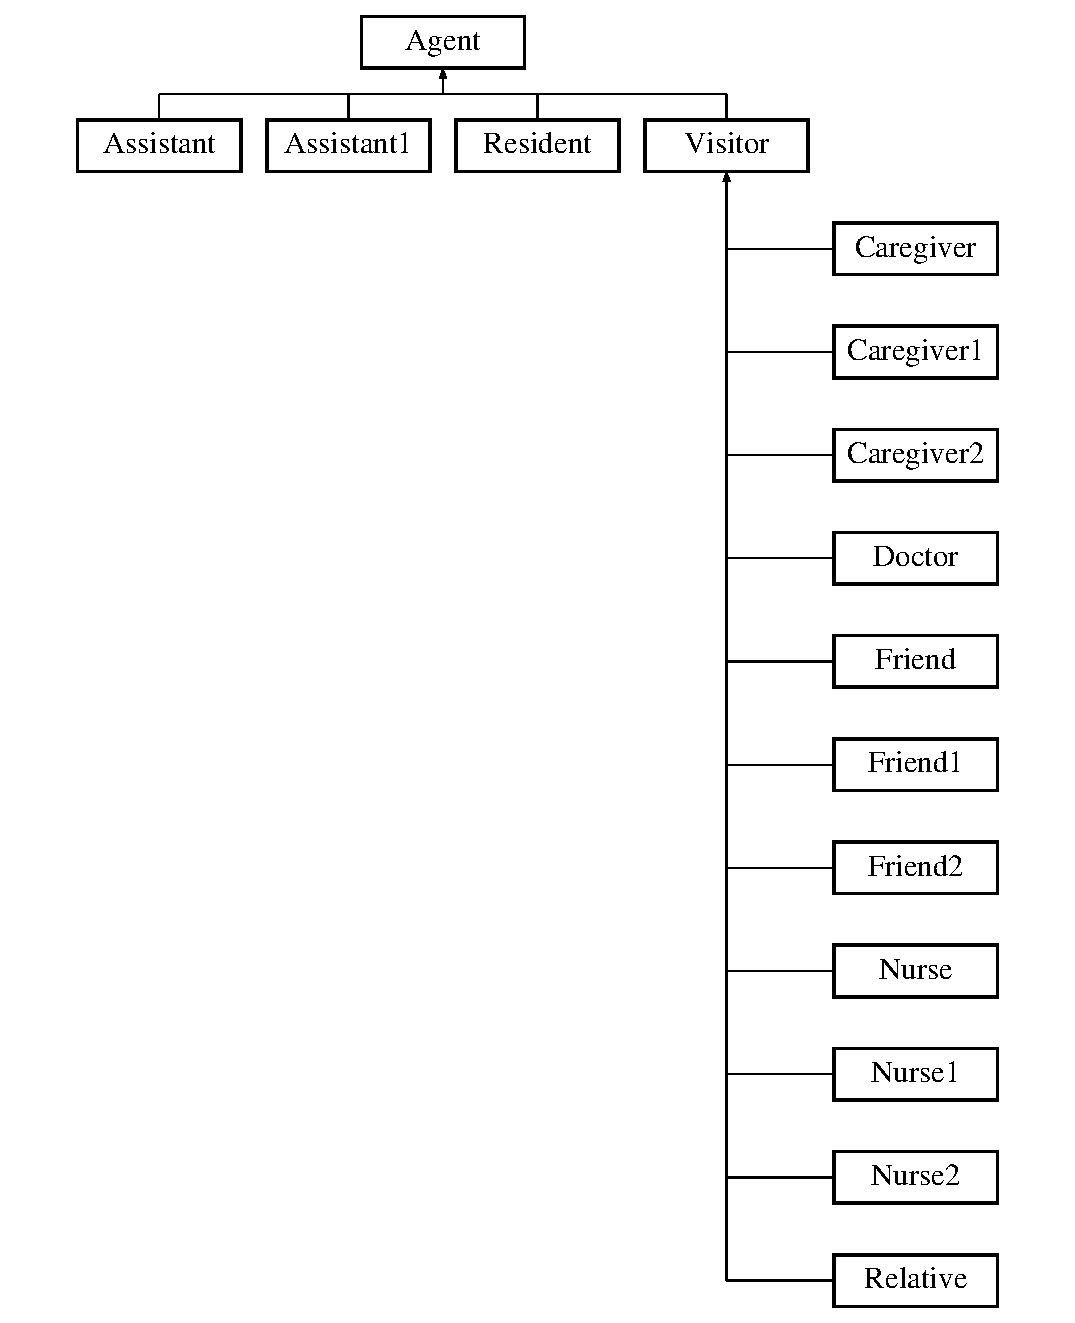
\includegraphics[height=3.000000cm]{classAgent}
\end{center}
\end{figure}
\subsection*{Public Member Functions}
\begin{DoxyCompactItemize}
\item 
\hypertarget{classAgent_a4b1182b9ee5dccaa871d71beef94a7d2}{virtual void {\bfseries Stage\-Odom\-\_\-callback} (nav\-\_\-msgs\-::\-Odometry msg)=0}\label{classAgent_a4b1182b9ee5dccaa871d71beef94a7d2}

\item 
\hypertarget{classAgent_adfe1de8bbeaa7e4a5f7f2ff3e45593e8}{virtual void {\bfseries Stage\-Laser\-\_\-callback} (sensor\-\_\-msgs\-::\-Laser\-Scan msg)=0}\label{classAgent_adfe1de8bbeaa7e4a5f7f2ff3e45593e8}

\item 
\hypertarget{classAgent_a70ae922d9ff12642634489b91ee5dbdf}{virtual int {\bfseries run} (int argc, char $\ast$$\ast$argv)=0}\label{classAgent_a70ae922d9ff12642634489b91ee5dbdf}

\end{DoxyCompactItemize}
\subsection*{Protected Types}
\begin{DoxyCompactItemize}
\item 
enum {\bfseries Type} \{ \\*
{\bfseries F\-R\-I\-E\-N\-D}, 
{\bfseries R\-E\-L\-A\-T\-I\-V\-E}, 
{\bfseries D\-O\-C\-T\-O\-R}, 
{\bfseries N\-U\-R\-S\-E}, 
\\*
{\bfseries C\-A\-R\-E\-G\-I\-V\-E\-R}, 
{\bfseries A\-S\-S\-I\-S\-T\-A\-N\-T}, 
{\bfseries R\-E\-S\-I\-D\-E\-N\-T}
 \}
\end{DoxyCompactItemize}
\subsection*{Protected Attributes}
\begin{DoxyCompactItemize}
\item 
\hypertarget{classAgent_a77dfc60513d8c90b2848297e09fffba7}{double {\bfseries linear\-\_\-x}}\label{classAgent_a77dfc60513d8c90b2848297e09fffba7}

\item 
\hypertarget{classAgent_affc842049c5010a5f8bd99a62d650a25}{double {\bfseries angular\-\_\-z}}\label{classAgent_affc842049c5010a5f8bd99a62d650a25}

\item 
\hypertarget{classAgent_af51536ae3b511b53726b84b9226cc772}{double {\bfseries px}}\label{classAgent_af51536ae3b511b53726b84b9226cc772}

\item 
\hypertarget{classAgent_a048e8b32d02a2fd58f046a444a287015}{double {\bfseries py}}\label{classAgent_a048e8b32d02a2fd58f046a444a287015}

\item 
\hypertarget{classAgent_aefcf2085a669d7e91d932e7cc3ee88ce}{int {\bfseries robot\-\_\-id}}\label{classAgent_aefcf2085a669d7e91d932e7cc3ee88ce}

\end{DoxyCompactItemize}


The documentation for this class was generated from the following file\-:\begin{DoxyCompactItemize}
\item 
se306\-\_\-project1/src/Agent.\-h\end{DoxyCompactItemize}

\hypertarget{classAgentFactory}{\section{Agent\-Factory Class Reference}
\label{classAgentFactory}\index{Agent\-Factory@{Agent\-Factory}}
}


Class for instantiating agents dynamically.  




{\ttfamily \#include $<$Agent\-Factory.\-h$>$}

\subsection*{Public Member Functions}
\begin{DoxyCompactItemize}
\item 
\hypertarget{classAgentFactory_a8785d71f067068f09326b4c5af5007b4}{void \hyperlink{classAgentFactory_a8785d71f067068f09326b4c5af5007b4}{create\-Mock\-Agent} ()}\label{classAgentFactory_a8785d71f067068f09326b4c5af5007b4}

\begin{DoxyCompactList}\small\item\em Creates a mock agent -\/ for testing. \end{DoxyCompactList}\item 
\hypertarget{classAgentFactory_aa8899b46f620a9a31f3e40041759ae24}{int {\bfseries create\-Agent} (Agent\-Const\-::\-Agent\-Type agent\-Type, int node\-Number)}\label{classAgentFactory_aa8899b46f620a9a31f3e40041759ae24}

\end{DoxyCompactItemize}


\subsection{Detailed Description}
Class for instantiating agents dynamically. 

The documentation for this class was generated from the following files\-:\begin{DoxyCompactItemize}
\item 
se306\-\_\-project1/src/Agent\-Factory.\-h\item 
se306\-\_\-project1/src/Agent\-Factory.\-cpp\end{DoxyCompactItemize}

\hypertarget{classAssistant}{\section{Assistant Class Reference}
\label{classAssistant}\index{Assistant@{Assistant}}
}


Class for robot assistants.  




{\ttfamily \#include $<$Assistant.\-h$>$}

Inheritance diagram for Assistant\-:\begin{figure}[H]
\begin{center}
\leavevmode
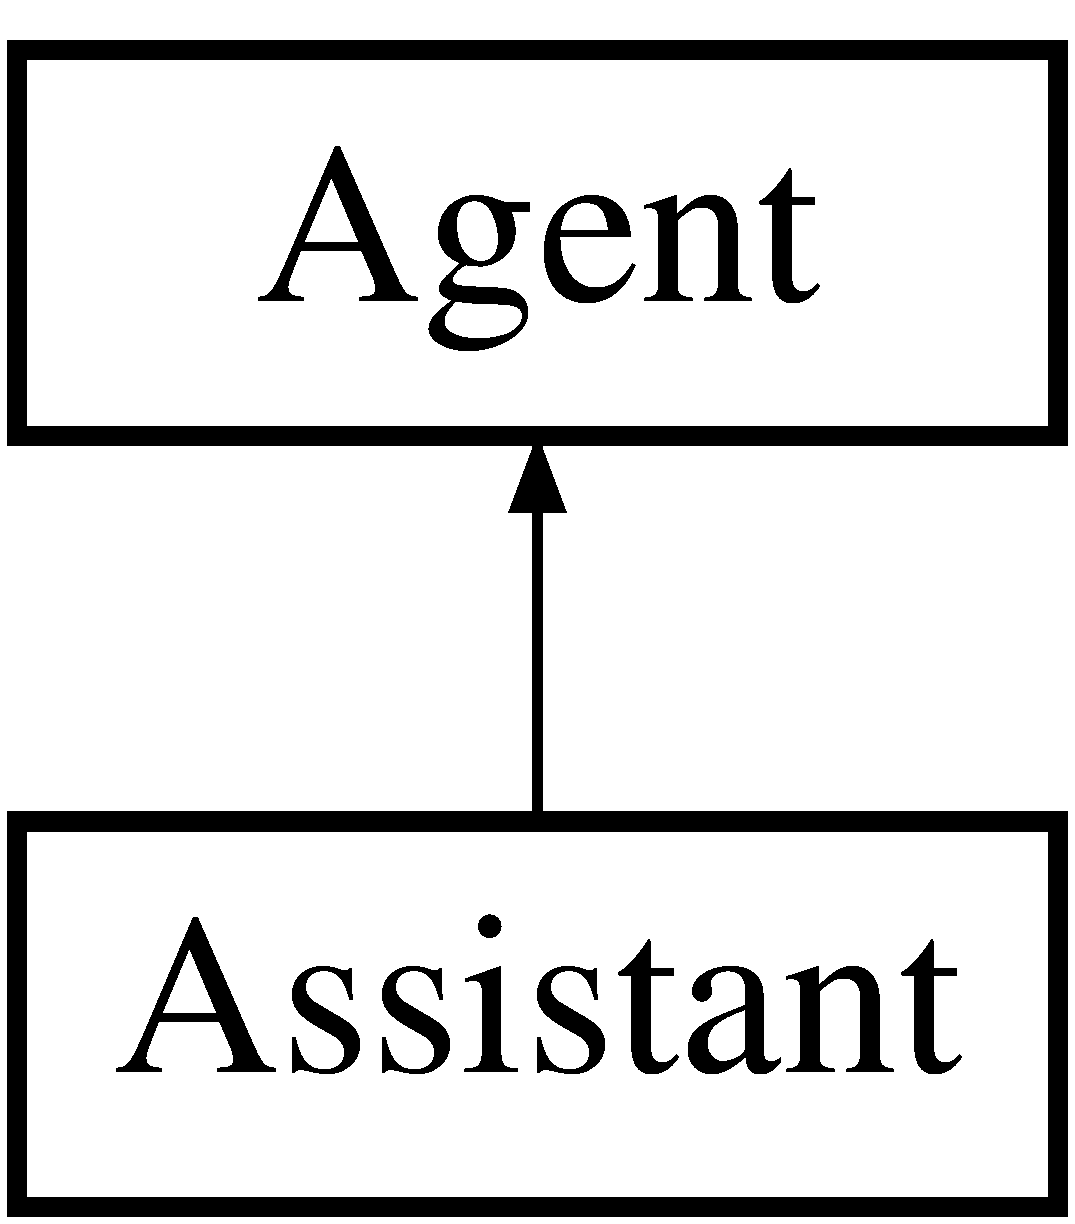
\includegraphics[height=2.000000cm]{classAssistant}
\end{center}
\end{figure}
\subsection*{Public Member Functions}
\begin{DoxyCompactItemize}
\item 
void \hyperlink{classAssistant_ad016061136f3fa5c3ed733e23a54aa00}{Stage\-Odom\-\_\-callback} (nav\-\_\-msgs\-::\-Odometry msg)
\begin{DoxyCompactList}\small\item\em Updates the \hyperlink{classAssistant}{Assistant}'s x position, y position, and angle to reflect its current pose. \end{DoxyCompactList}\item 
void \hyperlink{classAssistant_aaf1fe61dc3d3aac3f0ec603531ad9ad7}{Stage\-Laser\-\_\-callback} (sensor\-\_\-msgs\-::\-Laser\-Scan msg)
\begin{DoxyCompactList}\small\item\em Callback function to process laser scan messsages. You can access the range data from msg.\-ranges\mbox{[}i\mbox{]}. i = sample number. \end{DoxyCompactList}\item 
\hypertarget{classAssistant_a50eec4c3693b7b2c7d363ef4848a5815}{int \hyperlink{classAssistant_a50eec4c3693b7b2c7d363ef4848a5815}{run} (int argc, char $\ast$$\ast$argv)}\label{classAssistant_a50eec4c3693b7b2c7d363ef4848a5815}

\begin{DoxyCompactList}\small\item\em Main function for the \hyperlink{classAssistant}{Assistant} process. Controls node setup and periodic events. \end{DoxyCompactList}\item 
double \hyperlink{classAssistant_a8fce345025f32bcd0e45d83960d4b3f7}{calc\-\_\-goal\-\_\-angle} (double \hyperlink{classAssistant_a1a1f1fe48d0eb6a6a39b7fbdb2ef6641}{goal\-\_\-x}, double \hyperlink{classAssistant_a1b6ce5d7c3124140be8d351c847fe91c}{goal\-\_\-y}, double \hyperlink{classAssistant_a451a20f551c43d0b6810c8208fe84773}{cur\-\_\-angle}, double \hyperlink{classAssistant_a694fdaa5fb378340c42b7f75716cd1ce}{px}, double \hyperlink{classAssistant_ae092b444c226b5ffbdf454ad24f630d6}{py})
\begin{DoxyCompactList}\small\item\em Given the agent's current angle, this function calculates the angle to the goal. cur\-\_\-angle, goal\-\_\-x, goal\-\_\-y, px, and py are class fields but are also passed as parameters. \end{DoxyCompactList}\item 
std\-::pair$<$ double, double $>$ \hyperlink{classAssistant_ac420c9d5551f0ef6925d9a58a5b4854a}{move} (double \hyperlink{classAssistant_a1a1f1fe48d0eb6a6a39b7fbdb2ef6641}{goal\-\_\-x}, double \hyperlink{classAssistant_a1b6ce5d7c3124140be8d351c847fe91c}{goal\-\_\-y}, double \hyperlink{classAssistant_a451a20f551c43d0b6810c8208fe84773}{cur\-\_\-angle}, double \hyperlink{classAssistant_ae4468e02db193f0ffa0ca17a249f802d}{goal\-\_\-angle}, double \hyperlink{classAssistant_a694fdaa5fb378340c42b7f75716cd1ce}{px}, double \hyperlink{classAssistant_ae092b444c226b5ffbdf454ad24f630d6}{py})
\begin{DoxyCompactList}\small\item\em Keeps the agent moving by changing linear\-\_\-x ad angular\-\_\-z. \end{DoxyCompactList}\item 
\hypertarget{classAssistant_a320ca71cccf4964b341820db82b4b604}{void {\bfseries random\-Checkpoint\-Callback} (const ros\-::\-Timer\-Event \&)}\label{classAssistant_a320ca71cccf4964b341820db82b4b604}

\item 
std\-::pair$<$ double, double $>$ \hyperlink{classAssistant_a921c4b094867a4ebc62e404e772d002c}{move\-Path} (int path\mbox{[}$\,$\mbox{]}\mbox{[}2\mbox{]}, int path\-Length)
\begin{DoxyCompactList}\small\item\em Causes the agent to move until the goal is reached. When the goal is reached, the next checkpoint becomes the goal or if the list of checkpoints is exhausted, the agent returns to its initial position (the first checkpoint) \end{DoxyCompactList}\item 
void \hyperlink{classAssistant_ae4f0887ad0748940571fdf9ed1013766}{resident\-Status\-Callback} (\hyperlink{structse306__project1_1_1ResidentMsg__}{se306\-\_\-project1\-::\-Resident\-Msg} msg)
\begin{DoxyCompactList}\small\item\em Callback function that unpacks and processes resident status messages. \hyperlink{classAssistant}{Assistant} should subscribe to the Resident\-Msg topic in order for this callback to be called. Resident\-Msg is published by the \hyperlink{classResident}{Resident}. \end{DoxyCompactList}\item 
void \hyperlink{classAssistant_ae9b3476194ec440164926085a87a81f0}{medication\-Callback} (const ros\-::\-Timer\-Event \&)
\begin{DoxyCompactList}\small\item\em Periodic callback for the provision of medication that should act as a model for all periodic events. Called by the ros\-::\-Timer in the \hyperlink{classAssistant_a50eec4c3693b7b2c7d363ef4848a5815}{run()} function. Can specify start time, end time, and period. \end{DoxyCompactList}\end{DoxyCompactItemize}
\subsection*{Protected Attributes}
\begin{DoxyCompactItemize}
\item 
int \hyperlink{classAssistant_a13877ed73a684f59171c686186110870}{health}
\item 
int \hyperlink{classAssistant_a1f237fcda74950177c10cc26ea778863}{boredom}
\item 
int \hyperlink{classAssistant_ad109fd18cc762f9b9f7e64b626ec5d48}{hunger}
\item 
double \hyperlink{classAssistant_a1a1f1fe48d0eb6a6a39b7fbdb2ef6641}{goal\-\_\-x}
\item 
double \hyperlink{classAssistant_a1b6ce5d7c3124140be8d351c847fe91c}{goal\-\_\-y}
\item 
double \hyperlink{classAssistant_a694fdaa5fb378340c42b7f75716cd1ce}{px}
\item 
double \hyperlink{classAssistant_ae092b444c226b5ffbdf454ad24f630d6}{py}
\item 
double \hyperlink{classAssistant_ae4468e02db193f0ffa0ca17a249f802d}{goal\-\_\-angle}
\item 
\hypertarget{classAssistant_a23a1a8275bd6637f9d51e64fc77541d9}{bool {\bfseries running}}\label{classAssistant_a23a1a8275bd6637f9d51e64fc77541d9}

\item 
bool \hyperlink{classAssistant_a939484adfb9673d2608282124ef348b9}{is\-Set}
\item 
double \hyperlink{classAssistant_a451a20f551c43d0b6810c8208fe84773}{cur\-\_\-angle}
\item 
\hypertarget{classAssistant_a6ab1f06230072f8b32d6a0a7c8421f6e}{int {\bfseries cc}}\label{classAssistant_a6ab1f06230072f8b32d6a0a7c8421f6e}

\item 
\hypertarget{classAssistant_af2f914caf84e27c9e14fdb2367ef9efe}{bool {\bfseries is\-\_\-called}}\label{classAssistant_af2f914caf84e27c9e14fdb2367ef9efe}

\item 
\hypertarget{classAssistant_ab02623d3ac8868e28de116fe0b00f509}{std\-::pair$<$ double, bool $>$ {\bfseries goal\-\_\-pair}}\label{classAssistant_ab02623d3ac8868e28de116fe0b00f509}

\item 
std\-::pair$<$ double, double $>$ \hyperlink{classAssistant_a741527493a17d0f6dc512c03a2055fc1}{ret}
\item 
int \hyperlink{classAssistant_a31e94c37f8c6509b81c5c92ad5213e3f}{checkpoints} \mbox{[}11\mbox{]}\mbox{[}2\mbox{]}
\begin{DoxyCompactList}\small\item\em Set of checkpoints that the nodes can move to in the map. Gives x position and y position for each co-\/ordinate. \end{DoxyCompactList}\item 
bool \hyperlink{classAssistant_af9a992d4b1c5036ed73c57c7e1c5c258}{cooking}
\end{DoxyCompactItemize}
\subsection*{Additional Inherited Members}


\subsection{Detailed Description}
Class for robot assistants. 

\subsection{Member Function Documentation}
\hypertarget{classAssistant_a8fce345025f32bcd0e45d83960d4b3f7}{\index{Assistant@{Assistant}!calc\-\_\-goal\-\_\-angle@{calc\-\_\-goal\-\_\-angle}}
\index{calc\-\_\-goal\-\_\-angle@{calc\-\_\-goal\-\_\-angle}!Assistant@{Assistant}}
\subsubsection[{calc\-\_\-goal\-\_\-angle}]{\setlength{\rightskip}{0pt plus 5cm}double Assistant\-::calc\-\_\-goal\-\_\-angle (
\begin{DoxyParamCaption}
\item[{double}]{goal\-\_\-x, }
\item[{double}]{goal\-\_\-y, }
\item[{double}]{cur\-\_\-angle, }
\item[{double}]{px, }
\item[{double}]{py}
\end{DoxyParamCaption}
)}}\label{classAssistant_a8fce345025f32bcd0e45d83960d4b3f7}


Given the agent's current angle, this function calculates the angle to the goal. cur\-\_\-angle, goal\-\_\-x, goal\-\_\-y, px, and py are class fields but are also passed as parameters. 


\begin{DoxyParams}{Parameters}
{\em goal\-\_\-x} & The x co-\/ordinate of the goal \\
\hline
{\em goal\-\_\-y} & The y co-\/ordinate of the goal \\
\hline
{\em cur\-\_\-angle} & The agent's current angle, in reference to the co-\/ordinate system \\
\hline
{\em px} & The agent's initial x position \\
\hline
{\em py} & The agent's initial y position \\
\hline
{\em goal\-\_\-angle} & The angle that the robot must rotate to face the goal, in reference to the co-\/ordinate system. \\
\hline
\end{DoxyParams}
\hypertarget{classAssistant_ae9b3476194ec440164926085a87a81f0}{\index{Assistant@{Assistant}!medication\-Callback@{medication\-Callback}}
\index{medication\-Callback@{medication\-Callback}!Assistant@{Assistant}}
\subsubsection[{medication\-Callback}]{\setlength{\rightskip}{0pt plus 5cm}void Assistant\-::medication\-Callback (
\begin{DoxyParamCaption}
\item[{const ros\-::\-Timer\-Event \&}]{}
\end{DoxyParamCaption}
)}}\label{classAssistant_ae9b3476194ec440164926085a87a81f0}


Periodic callback for the provision of medication that should act as a model for all periodic events. Called by the ros\-::\-Timer in the \hyperlink{classAssistant_a50eec4c3693b7b2c7d363ef4848a5815}{run()} function. Can specify start time, end time, and period. 

\begin{DoxyNote}{Note}
The callback is called at the end of the duration specified for the timer. 
\end{DoxyNote}
\begin{DoxyRemark}{Remarks}
This could be adjustd in the future to allow for events that occur only on certain days -\/ currently it accommodates only for events that occur every x days (or multiple times per day). 
\end{DoxyRemark}

\begin{DoxyParams}{Parameters}
{\em Timer\-Event\&} & Timer\-Event generated by a ros\-::\-Timer. \\
\hline
\end{DoxyParams}
\hypertarget{classAssistant_ac420c9d5551f0ef6925d9a58a5b4854a}{\index{Assistant@{Assistant}!move@{move}}
\index{move@{move}!Assistant@{Assistant}}
\subsubsection[{move}]{\setlength{\rightskip}{0pt plus 5cm}std\-::pair$<$ double, double $>$ Assistant\-::move (
\begin{DoxyParamCaption}
\item[{double}]{goal\-\_\-x, }
\item[{double}]{goal\-\_\-y, }
\item[{double}]{cur\-\_\-angle, }
\item[{double}]{goal\-\_\-angle, }
\item[{double}]{px, }
\item[{double}]{py}
\end{DoxyParamCaption}
)}}\label{classAssistant_ac420c9d5551f0ef6925d9a58a5b4854a}


Keeps the agent moving by changing linear\-\_\-x ad angular\-\_\-z. 


\begin{DoxyParams}{Parameters}
{\em goal\-\_\-x} & The x position of the robot's goal \\
\hline
{\em goal\-\_\-y} & The y position of the robot's goal \\
\hline
{\em cur\-\_\-angle} & The agent's current facing, in reference to the co-\/ordinate system. \\
\hline
{\em goal\-\_\-angle} & The angle that the agent must face in order to reach the goal. \\
\hline
{\em px} & Initial x position \\
\hline
{\em py} & Initial y position \\
\hline
\end{DoxyParams}
\begin{DoxyReturn}{Returns}
\-\_\-ret linear\-\_\-x and angular\-\_\-z 
\end{DoxyReturn}
\hypertarget{classAssistant_a921c4b094867a4ebc62e404e772d002c}{\index{Assistant@{Assistant}!move\-Path@{move\-Path}}
\index{move\-Path@{move\-Path}!Assistant@{Assistant}}
\subsubsection[{move\-Path}]{\setlength{\rightskip}{0pt plus 5cm}std\-::pair$<$ double, double $>$ Assistant\-::move\-Path (
\begin{DoxyParamCaption}
\item[{int}]{path\mbox{[}$\,$\mbox{]}\mbox{[}2\mbox{]}, }
\item[{int}]{path\-Length}
\end{DoxyParamCaption}
)}}\label{classAssistant_a921c4b094867a4ebc62e404e772d002c}


Causes the agent to move until the goal is reached. When the goal is reached, the next checkpoint becomes the goal or if the list of checkpoints is exhausted, the agent returns to its initial position (the first checkpoint) 


\begin{DoxyParams}{Parameters}
{\em path\mbox{[}$\,$\mbox{]}\mbox{[}2\mbox{]}} & An array of checkpoints that forms a path. \\
\hline
{\em path\-Length} & The number of checkpoints in the path (-\/1, as counting starts at 0) \\
\hline
\end{DoxyParams}
\begin{DoxyReturn}{Returns}
linear\-\_\-x and angular\-\_\-z 
\end{DoxyReturn}
\hypertarget{classAssistant_ae4f0887ad0748940571fdf9ed1013766}{\index{Assistant@{Assistant}!resident\-Status\-Callback@{resident\-Status\-Callback}}
\index{resident\-Status\-Callback@{resident\-Status\-Callback}!Assistant@{Assistant}}
\subsubsection[{resident\-Status\-Callback}]{\setlength{\rightskip}{0pt plus 5cm}void Assistant\-::resident\-Status\-Callback (
\begin{DoxyParamCaption}
\item[{{\bf se306\-\_\-project1\-::\-Resident\-Msg}}]{msg}
\end{DoxyParamCaption}
)}}\label{classAssistant_ae4f0887ad0748940571fdf9ed1013766}


Callback function that unpacks and processes resident status messages. \hyperlink{classAssistant}{Assistant} should subscribe to the Resident\-Msg topic in order for this callback to be called. Resident\-Msg is published by the \hyperlink{classResident}{Resident}. 

\begin{DoxyNote}{Note}
Currently this callback processes only resident hunger, controlling the cooking behaviour. More behaviours can be implemented later. 
\end{DoxyNote}

\begin{DoxyParams}{Parameters}
{\em msg} & A custom Resident\-Msg message that contains information about the resident's current status. \\
\hline
\end{DoxyParams}
\hypertarget{classAssistant_aaf1fe61dc3d3aac3f0ec603531ad9ad7}{\index{Assistant@{Assistant}!Stage\-Laser\-\_\-callback@{Stage\-Laser\-\_\-callback}}
\index{Stage\-Laser\-\_\-callback@{Stage\-Laser\-\_\-callback}!Assistant@{Assistant}}
\subsubsection[{Stage\-Laser\-\_\-callback}]{\setlength{\rightskip}{0pt plus 5cm}void Assistant\-::\-Stage\-Laser\-\_\-callback (
\begin{DoxyParamCaption}
\item[{sensor\-\_\-msgs\-::\-Laser\-Scan}]{msg}
\end{DoxyParamCaption}
)\hspace{0.3cm}{\ttfamily [virtual]}}}\label{classAssistant_aaf1fe61dc3d3aac3f0ec603531ad9ad7}


Callback function to process laser scan messsages. You can access the range data from msg.\-ranges\mbox{[}i\mbox{]}. i = sample number. 

\begin{DoxyNote}{Note}
Currently blank as it is not in use. Navigation operates through a checkpoint system. 
\end{DoxyNote}

\begin{DoxyParams}{Parameters}
{\em msg} & Single scan from a planar laser range finder \\
\hline
\end{DoxyParams}


Implements \hyperlink{classAgent}{Agent}.

\hypertarget{classAssistant_ad016061136f3fa5c3ed733e23a54aa00}{\index{Assistant@{Assistant}!Stage\-Odom\-\_\-callback@{Stage\-Odom\-\_\-callback}}
\index{Stage\-Odom\-\_\-callback@{Stage\-Odom\-\_\-callback}!Assistant@{Assistant}}
\subsubsection[{Stage\-Odom\-\_\-callback}]{\setlength{\rightskip}{0pt plus 5cm}void Assistant\-::\-Stage\-Odom\-\_\-callback (
\begin{DoxyParamCaption}
\item[{nav\-\_\-msgs\-::\-Odometry}]{msg}
\end{DoxyParamCaption}
)\hspace{0.3cm}{\ttfamily [virtual]}}}\label{classAssistant_ad016061136f3fa5c3ed733e23a54aa00}


Updates the \hyperlink{classAssistant}{Assistant}'s x position, y position, and angle to reflect its current pose. 

\begin{DoxyNote}{Note}
Rounding is used to calculate the current angle. This approximation is accounted for by using threshholds when processing angles. 
\end{DoxyNote}

\begin{DoxyParams}{Parameters}
{\em msg} & Odometry message from odom topic \\
\hline
\end{DoxyParams}


Implements \hyperlink{classAgent}{Agent}.



\subsection{Member Data Documentation}
\hypertarget{classAssistant_a1f237fcda74950177c10cc26ea778863}{\index{Assistant@{Assistant}!boredom@{boredom}}
\index{boredom@{boredom}!Assistant@{Assistant}}
\subsubsection[{boredom}]{\setlength{\rightskip}{0pt plus 5cm}int Assistant\-::boredom\hspace{0.3cm}{\ttfamily [protected]}}}\label{classAssistant_a1f237fcda74950177c10cc26ea778863}
\hyperlink{classResident}{Resident} boredom \hypertarget{classAssistant_a31e94c37f8c6509b81c5c92ad5213e3f}{\index{Assistant@{Assistant}!checkpoints@{checkpoints}}
\index{checkpoints@{checkpoints}!Assistant@{Assistant}}
\subsubsection[{checkpoints}]{\setlength{\rightskip}{0pt plus 5cm}int Assistant\-::checkpoints\mbox{[}11\mbox{]}\mbox{[}2\mbox{]}\hspace{0.3cm}{\ttfamily [protected]}}}\label{classAssistant_a31e94c37f8c6509b81c5c92ad5213e3f}
{\bfseries Initial value\-:}
\begin{DoxyCode}
= \{  
        \{30, 25\},
        \{30, 7\}, 
        \{40, 7\},
        \{40, 8\},
        \{38,8\},
        \{38,7\},
        \{40,7\},
        \{30,7\},
        \{30, 25\},
        \{34,20\},
        \{30, 25\}
        \}
\end{DoxyCode}


Set of checkpoints that the nodes can move to in the map. Gives x position and y position for each co-\/ordinate. 

\hypertarget{classAssistant_af9a992d4b1c5036ed73c57c7e1c5c258}{\index{Assistant@{Assistant}!cooking@{cooking}}
\index{cooking@{cooking}!Assistant@{Assistant}}
\subsubsection[{cooking}]{\setlength{\rightskip}{0pt plus 5cm}bool Assistant\-::cooking\hspace{0.3cm}{\ttfamily [protected]}}}\label{classAssistant_af9a992d4b1c5036ed73c57c7e1c5c258}
True if the robot is cooking \hypertarget{classAssistant_a451a20f551c43d0b6810c8208fe84773}{\index{Assistant@{Assistant}!cur\-\_\-angle@{cur\-\_\-angle}}
\index{cur\-\_\-angle@{cur\-\_\-angle}!Assistant@{Assistant}}
\subsubsection[{cur\-\_\-angle}]{\setlength{\rightskip}{0pt plus 5cm}double Assistant\-::cur\-\_\-angle\hspace{0.3cm}{\ttfamily [protected]}}}\label{classAssistant_a451a20f551c43d0b6810c8208fe84773}
The robot's current facing in reference to the co-\/ordinate system \hypertarget{classAssistant_ae4468e02db193f0ffa0ca17a249f802d}{\index{Assistant@{Assistant}!goal\-\_\-angle@{goal\-\_\-angle}}
\index{goal\-\_\-angle@{goal\-\_\-angle}!Assistant@{Assistant}}
\subsubsection[{goal\-\_\-angle}]{\setlength{\rightskip}{0pt plus 5cm}double Assistant\-::goal\-\_\-angle\hspace{0.3cm}{\ttfamily [protected]}}}\label{classAssistant_ae4468e02db193f0ffa0ca17a249f802d}
The angle that the robot must face to approach the goal, defined in reference to the co-\/ordinate system \hypertarget{classAssistant_a1a1f1fe48d0eb6a6a39b7fbdb2ef6641}{\index{Assistant@{Assistant}!goal\-\_\-x@{goal\-\_\-x}}
\index{goal\-\_\-x@{goal\-\_\-x}!Assistant@{Assistant}}
\subsubsection[{goal\-\_\-x}]{\setlength{\rightskip}{0pt plus 5cm}double Assistant\-::goal\-\_\-x\hspace{0.3cm}{\ttfamily [protected]}}}\label{classAssistant_a1a1f1fe48d0eb6a6a39b7fbdb2ef6641}
The x position of the robot's goal \hypertarget{classAssistant_a1b6ce5d7c3124140be8d351c847fe91c}{\index{Assistant@{Assistant}!goal\-\_\-y@{goal\-\_\-y}}
\index{goal\-\_\-y@{goal\-\_\-y}!Assistant@{Assistant}}
\subsubsection[{goal\-\_\-y}]{\setlength{\rightskip}{0pt plus 5cm}double Assistant\-::goal\-\_\-y\hspace{0.3cm}{\ttfamily [protected]}}}\label{classAssistant_a1b6ce5d7c3124140be8d351c847fe91c}
The y position of the robot's goal \hypertarget{classAssistant_a13877ed73a684f59171c686186110870}{\index{Assistant@{Assistant}!health@{health}}
\index{health@{health}!Assistant@{Assistant}}
\subsubsection[{health}]{\setlength{\rightskip}{0pt plus 5cm}int Assistant\-::health\hspace{0.3cm}{\ttfamily [protected]}}}\label{classAssistant_a13877ed73a684f59171c686186110870}
\hyperlink{classResident}{Resident} health \hypertarget{classAssistant_ad109fd18cc762f9b9f7e64b626ec5d48}{\index{Assistant@{Assistant}!hunger@{hunger}}
\index{hunger@{hunger}!Assistant@{Assistant}}
\subsubsection[{hunger}]{\setlength{\rightskip}{0pt plus 5cm}int Assistant\-::hunger\hspace{0.3cm}{\ttfamily [protected]}}}\label{classAssistant_ad109fd18cc762f9b9f7e64b626ec5d48}
\hyperlink{classResident}{Resident} hunger \hypertarget{classAssistant_a939484adfb9673d2608282124ef348b9}{\index{Assistant@{Assistant}!is\-Set@{is\-Set}}
\index{is\-Set@{is\-Set}!Assistant@{Assistant}}
\subsubsection[{is\-Set}]{\setlength{\rightskip}{0pt plus 5cm}bool Assistant\-::is\-Set\hspace{0.3cm}{\ttfamily [protected]}}}\label{classAssistant_a939484adfb9673d2608282124ef348b9}
Indicates whether the robot is currently on its way to a goal. \hypertarget{classAssistant_a694fdaa5fb378340c42b7f75716cd1ce}{\index{Assistant@{Assistant}!px@{px}}
\index{px@{px}!Assistant@{Assistant}}
\subsubsection[{px}]{\setlength{\rightskip}{0pt plus 5cm}double Assistant\-::px\hspace{0.3cm}{\ttfamily [protected]}}}\label{classAssistant_a694fdaa5fb378340c42b7f75716cd1ce}
The robot's initial x position \hypertarget{classAssistant_ae092b444c226b5ffbdf454ad24f630d6}{\index{Assistant@{Assistant}!py@{py}}
\index{py@{py}!Assistant@{Assistant}}
\subsubsection[{py}]{\setlength{\rightskip}{0pt plus 5cm}double Assistant\-::py\hspace{0.3cm}{\ttfamily [protected]}}}\label{classAssistant_ae092b444c226b5ffbdf454ad24f630d6}
The robot's initial y position \hypertarget{classAssistant_a741527493a17d0f6dc512c03a2055fc1}{\index{Assistant@{Assistant}!ret@{ret}}
\index{ret@{ret}!Assistant@{Assistant}}
\subsubsection[{ret}]{\setlength{\rightskip}{0pt plus 5cm}std\-::pair$<$double, double$>$ Assistant\-::ret\hspace{0.3cm}{\ttfamily [protected]}}}\label{classAssistant_a741527493a17d0f6dc512c03a2055fc1}
linear\-\_\-x and angular\-\_\-z for the robot 

The documentation for this class was generated from the following files\-:\begin{DoxyCompactItemize}
\item 
se306\-\_\-project1/src/Assistant.\-h\item 
se306\-\_\-project1/src/Assistant.\-cpp\end{DoxyCompactItemize}

\hypertarget{classAssistant1}{\section{Assistant1 Class Reference}
\label{classAssistant1}\index{Assistant1@{Assistant1}}
}


Class representing the \hyperlink{classAssistant}{Assistant}.  




{\ttfamily \#include $<$Assistant1.\-h$>$}

Inheritance diagram for Assistant1\-:\begin{figure}[H]
\begin{center}
\leavevmode
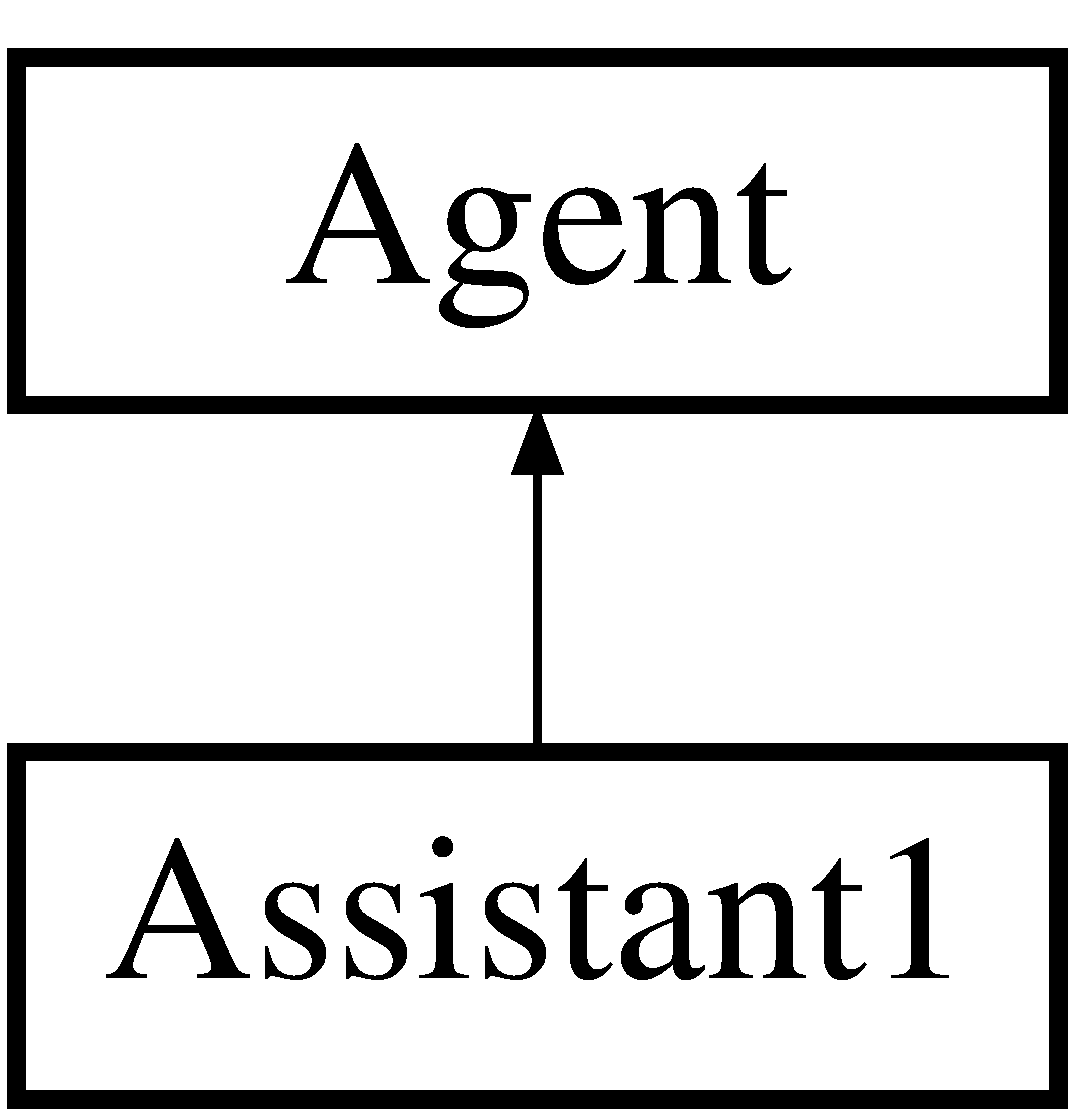
\includegraphics[height=2.000000cm]{classAssistant1}
\end{center}
\end{figure}
\subsection*{Public Member Functions}
\begin{DoxyCompactItemize}
\item 
int \hyperlink{classAssistant1_a4d20c44da8dfd96cda961d12ecf91058}{run} (int argc, char $\ast$argv\mbox{[}$\,$\mbox{]})
\begin{DoxyCompactList}\small\item\em Main function that controls agent events. \end{DoxyCompactList}\end{DoxyCompactItemize}
\subsection*{Additional Inherited Members}


\subsection{Detailed Description}
Class representing the \hyperlink{classAssistant}{Assistant}. 

\subsection{Member Function Documentation}
\hypertarget{classAssistant1_a4d20c44da8dfd96cda961d12ecf91058}{\index{Assistant1@{Assistant1}!run@{run}}
\index{run@{run}!Assistant1@{Assistant1}}
\subsubsection[{run}]{\setlength{\rightskip}{0pt plus 5cm}int Assistant1\-::run (
\begin{DoxyParamCaption}
\item[{int}]{argc, }
\item[{char $\ast$}]{argv\mbox{[}$\,$\mbox{]}}
\end{DoxyParamCaption}
)}}\label{classAssistant1_a4d20c44da8dfd96cda961d12ecf91058}


Main function that controls agent events. 

Main function for the \hyperlink{classAssistant}{Assistant} process. Controls node setup and periodic events. 

The documentation for this class was generated from the following files\-:\begin{DoxyCompactItemize}
\item 
se306\-\_\-project1/src/Assistant1.\-h\item 
se306\-\_\-project1/src/Assistant1.\-cpp\end{DoxyCompactItemize}

\hypertarget{classse306__project1_1_1msg_1_1__AssistantMsg_1_1AssistantMsg}{\section{se306\-\_\-project1.\-msg.\-\_\-\-Assistant\-Msg.\-Assistant\-Msg Class Reference}
\label{classse306__project1_1_1msg_1_1__AssistantMsg_1_1AssistantMsg}\index{se306\-\_\-project1.\-msg.\-\_\-\-Assistant\-Msg.\-Assistant\-Msg@{se306\-\_\-project1.\-msg.\-\_\-\-Assistant\-Msg.\-Assistant\-Msg}}
}
Inheritance diagram for se306\-\_\-project1.\-msg.\-\_\-\-Assistant\-Msg.\-Assistant\-Msg\-:\begin{figure}[H]
\begin{center}
\leavevmode
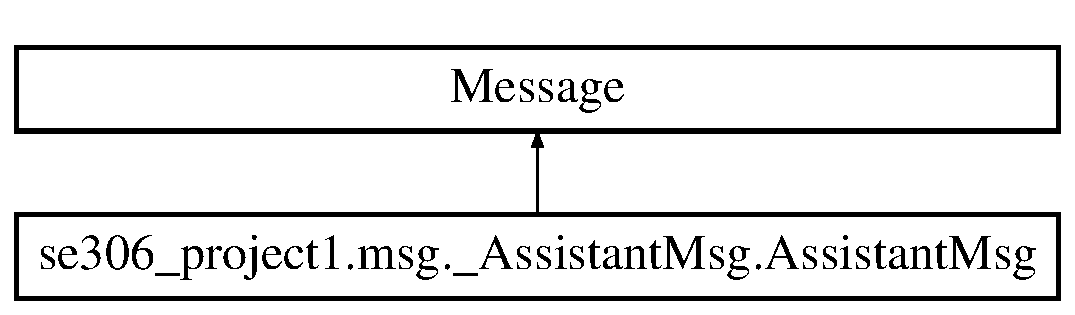
\includegraphics[height=2.000000cm]{classse306__project1_1_1msg_1_1__AssistantMsg_1_1AssistantMsg}
\end{center}
\end{figure}
\subsection*{Public Member Functions}
\begin{DoxyCompactItemize}
\item 
def \hyperlink{classse306__project1_1_1msg_1_1__AssistantMsg_1_1AssistantMsg_a301e2c6ab7ed4c48405f23e0992ad767}{\-\_\-\-\_\-init\-\_\-\-\_\-}
\item 
def \hyperlink{classse306__project1_1_1msg_1_1__AssistantMsg_1_1AssistantMsg_a8c4b6d99e72713a71f12f87c18ee2e06}{serialize}
\item 
def \hyperlink{classse306__project1_1_1msg_1_1__AssistantMsg_1_1AssistantMsg_aa8700e1054cba903da6a3e14051c4c04}{deserialize}
\item 
def \hyperlink{classse306__project1_1_1msg_1_1__AssistantMsg_1_1AssistantMsg_a6018ce827cc44ec27b28ef5c65380cfd}{serialize\-\_\-numpy}
\item 
def \hyperlink{classse306__project1_1_1msg_1_1__AssistantMsg_1_1AssistantMsg_a1572c60a75384a707bf4200a39a0a295}{deserialize\-\_\-numpy}
\end{DoxyCompactItemize}
\subsection*{Public Attributes}
\begin{DoxyCompactItemize}
\item 
\hypertarget{classse306__project1_1_1msg_1_1__AssistantMsg_1_1AssistantMsg_a7768eacfe92abe76d8497631b7f1b4ea}{{\bfseries cooking}}\label{classse306__project1_1_1msg_1_1__AssistantMsg_1_1AssistantMsg_a7768eacfe92abe76d8497631b7f1b4ea}

\end{DoxyCompactItemize}


\subsection{Constructor \& Destructor Documentation}
\hypertarget{classse306__project1_1_1msg_1_1__AssistantMsg_1_1AssistantMsg_a301e2c6ab7ed4c48405f23e0992ad767}{\index{se306\-\_\-project1\-::msg\-::\-\_\-\-Assistant\-Msg\-::\-Assistant\-Msg@{se306\-\_\-project1\-::msg\-::\-\_\-\-Assistant\-Msg\-::\-Assistant\-Msg}!\-\_\-\-\_\-init\-\_\-\-\_\-@{\-\_\-\-\_\-init\-\_\-\-\_\-}}
\index{\-\_\-\-\_\-init\-\_\-\-\_\-@{\-\_\-\-\_\-init\-\_\-\-\_\-}!se306_project1::msg::_AssistantMsg::AssistantMsg@{se306\-\_\-project1\-::msg\-::\-\_\-\-Assistant\-Msg\-::\-Assistant\-Msg}}
\subsubsection[{\-\_\-\-\_\-init\-\_\-\-\_\-}]{\setlength{\rightskip}{0pt plus 5cm}def se306\-\_\-project1.\-msg.\-\_\-\-Assistant\-Msg.\-Assistant\-Msg.\-\_\-\-\_\-init\-\_\-\-\_\- (
\begin{DoxyParamCaption}
\item[{}]{self, }
\item[{}]{args, }
\item[{}]{kwds}
\end{DoxyParamCaption}
)}}\label{classse306__project1_1_1msg_1_1__AssistantMsg_1_1AssistantMsg_a301e2c6ab7ed4c48405f23e0992ad767}
\begin{DoxyVerb}Constructor. Any message fields that are implicitly/explicitly
set to None will be assigned a default value. The recommend
use is keyword arguments as this is more robust to future message
changes.  You cannot mix in-order arguments and keyword arguments.

The available fields are:
   cooking

:param args: complete set of field values, in .msg order
:param kwds: use keyword arguments corresponding to message field names
to set specific fields.
\end{DoxyVerb}
 

\subsection{Member Function Documentation}
\hypertarget{classse306__project1_1_1msg_1_1__AssistantMsg_1_1AssistantMsg_aa8700e1054cba903da6a3e14051c4c04}{\index{se306\-\_\-project1\-::msg\-::\-\_\-\-Assistant\-Msg\-::\-Assistant\-Msg@{se306\-\_\-project1\-::msg\-::\-\_\-\-Assistant\-Msg\-::\-Assistant\-Msg}!deserialize@{deserialize}}
\index{deserialize@{deserialize}!se306_project1::msg::_AssistantMsg::AssistantMsg@{se306\-\_\-project1\-::msg\-::\-\_\-\-Assistant\-Msg\-::\-Assistant\-Msg}}
\subsubsection[{deserialize}]{\setlength{\rightskip}{0pt plus 5cm}def se306\-\_\-project1.\-msg.\-\_\-\-Assistant\-Msg.\-Assistant\-Msg.\-deserialize (
\begin{DoxyParamCaption}
\item[{}]{self, }
\item[{}]{str}
\end{DoxyParamCaption}
)}}\label{classse306__project1_1_1msg_1_1__AssistantMsg_1_1AssistantMsg_aa8700e1054cba903da6a3e14051c4c04}
\begin{DoxyVerb}unpack serialized message in str into this message instance
:param str: byte array of serialized message, ``str``
\end{DoxyVerb}
 \hypertarget{classse306__project1_1_1msg_1_1__AssistantMsg_1_1AssistantMsg_a1572c60a75384a707bf4200a39a0a295}{\index{se306\-\_\-project1\-::msg\-::\-\_\-\-Assistant\-Msg\-::\-Assistant\-Msg@{se306\-\_\-project1\-::msg\-::\-\_\-\-Assistant\-Msg\-::\-Assistant\-Msg}!deserialize\-\_\-numpy@{deserialize\-\_\-numpy}}
\index{deserialize\-\_\-numpy@{deserialize\-\_\-numpy}!se306_project1::msg::_AssistantMsg::AssistantMsg@{se306\-\_\-project1\-::msg\-::\-\_\-\-Assistant\-Msg\-::\-Assistant\-Msg}}
\subsubsection[{deserialize\-\_\-numpy}]{\setlength{\rightskip}{0pt plus 5cm}def se306\-\_\-project1.\-msg.\-\_\-\-Assistant\-Msg.\-Assistant\-Msg.\-deserialize\-\_\-numpy (
\begin{DoxyParamCaption}
\item[{}]{self, }
\item[{}]{str, }
\item[{}]{numpy}
\end{DoxyParamCaption}
)}}\label{classse306__project1_1_1msg_1_1__AssistantMsg_1_1AssistantMsg_a1572c60a75384a707bf4200a39a0a295}
\begin{DoxyVerb}unpack serialized message in str into this message instance using numpy for array types
:param str: byte array of serialized message, ``str``
:param numpy: numpy python module
\end{DoxyVerb}
 \hypertarget{classse306__project1_1_1msg_1_1__AssistantMsg_1_1AssistantMsg_a8c4b6d99e72713a71f12f87c18ee2e06}{\index{se306\-\_\-project1\-::msg\-::\-\_\-\-Assistant\-Msg\-::\-Assistant\-Msg@{se306\-\_\-project1\-::msg\-::\-\_\-\-Assistant\-Msg\-::\-Assistant\-Msg}!serialize@{serialize}}
\index{serialize@{serialize}!se306_project1::msg::_AssistantMsg::AssistantMsg@{se306\-\_\-project1\-::msg\-::\-\_\-\-Assistant\-Msg\-::\-Assistant\-Msg}}
\subsubsection[{serialize}]{\setlength{\rightskip}{0pt plus 5cm}def se306\-\_\-project1.\-msg.\-\_\-\-Assistant\-Msg.\-Assistant\-Msg.\-serialize (
\begin{DoxyParamCaption}
\item[{}]{self, }
\item[{}]{buff}
\end{DoxyParamCaption}
)}}\label{classse306__project1_1_1msg_1_1__AssistantMsg_1_1AssistantMsg_a8c4b6d99e72713a71f12f87c18ee2e06}
\begin{DoxyVerb}serialize message into buffer
:param buff: buffer, ``StringIO``
\end{DoxyVerb}
 \hypertarget{classse306__project1_1_1msg_1_1__AssistantMsg_1_1AssistantMsg_a6018ce827cc44ec27b28ef5c65380cfd}{\index{se306\-\_\-project1\-::msg\-::\-\_\-\-Assistant\-Msg\-::\-Assistant\-Msg@{se306\-\_\-project1\-::msg\-::\-\_\-\-Assistant\-Msg\-::\-Assistant\-Msg}!serialize\-\_\-numpy@{serialize\-\_\-numpy}}
\index{serialize\-\_\-numpy@{serialize\-\_\-numpy}!se306_project1::msg::_AssistantMsg::AssistantMsg@{se306\-\_\-project1\-::msg\-::\-\_\-\-Assistant\-Msg\-::\-Assistant\-Msg}}
\subsubsection[{serialize\-\_\-numpy}]{\setlength{\rightskip}{0pt plus 5cm}def se306\-\_\-project1.\-msg.\-\_\-\-Assistant\-Msg.\-Assistant\-Msg.\-serialize\-\_\-numpy (
\begin{DoxyParamCaption}
\item[{}]{self, }
\item[{}]{buff, }
\item[{}]{numpy}
\end{DoxyParamCaption}
)}}\label{classse306__project1_1_1msg_1_1__AssistantMsg_1_1AssistantMsg_a6018ce827cc44ec27b28ef5c65380cfd}
\begin{DoxyVerb}serialize message with numpy array types into buffer
:param buff: buffer, ``StringIO``
:param numpy: numpy python module
\end{DoxyVerb}
 

The documentation for this class was generated from the following file\-:\begin{DoxyCompactItemize}
\item 
se306\-\_\-project1/src/se306\-\_\-project1/msg/\-\_\-\-Assistant\-Msg.\-py\end{DoxyCompactItemize}

\hypertarget{structse306__project1_1_1AssistantMsg__}{\section{se306\-\_\-project1\-:\-:Assistant\-Msg\-\_\-$<$ Container\-Allocator $>$ Struct Template Reference}
\label{structse306__project1_1_1AssistantMsg__}\index{se306\-\_\-project1\-::\-Assistant\-Msg\-\_\-$<$ Container\-Allocator $>$@{se306\-\_\-project1\-::\-Assistant\-Msg\-\_\-$<$ Container\-Allocator $>$}}
}
\subsection*{Public Types}
\begin{DoxyCompactItemize}
\item 
\hypertarget{structse306__project1_1_1AssistantMsg___a1fd81595948c57178036f385b43b3e85}{typedef \hyperlink{structse306__project1_1_1AssistantMsg__}{Assistant\-Msg\-\_\-}\\*
$<$ Container\-Allocator $>$ {\bfseries Type}}\label{structse306__project1_1_1AssistantMsg___a1fd81595948c57178036f385b43b3e85}

\item 
\hypertarget{structse306__project1_1_1AssistantMsg___aec66b7b1d73c662979534e5c2b6b3c5b}{typedef int64\-\_\-t {\bfseries \-\_\-\-Food\-Delivered\-\_\-type}}\label{structse306__project1_1_1AssistantMsg___aec66b7b1d73c662979534e5c2b6b3c5b}

\item 
\hypertarget{structse306__project1_1_1AssistantMsg___ae4e951cbe451656c3432adc85dac1d27}{typedef boost\-::shared\-\_\-ptr\\*
$<$ \-::\hyperlink{structse306__project1_1_1AssistantMsg__}{se306\-\_\-project1\-::\-Assistant\-Msg\-\_\-}\\*
$<$ Container\-Allocator $>$ $>$ {\bfseries Ptr}}\label{structse306__project1_1_1AssistantMsg___ae4e951cbe451656c3432adc85dac1d27}

\item 
\hypertarget{structse306__project1_1_1AssistantMsg___a96808a76b3826b3fe60f4733c576bb10}{typedef boost\-::shared\-\_\-ptr\\*
$<$ \-::\hyperlink{structse306__project1_1_1AssistantMsg__}{se306\-\_\-project1\-::\-Assistant\-Msg\-\_\-}\\*
$<$ Container\-Allocator $>$ const  $>$ {\bfseries Const\-Ptr}}\label{structse306__project1_1_1AssistantMsg___a96808a76b3826b3fe60f4733c576bb10}

\end{DoxyCompactItemize}
\subsection*{Public Member Functions}
\begin{DoxyCompactItemize}
\item 
\hypertarget{structse306__project1_1_1AssistantMsg___af325d6761ff1fe9faf15d9191ecf30a9}{{\bfseries Assistant\-Msg\-\_\-} (const Container\-Allocator \&\-\_\-alloc)}\label{structse306__project1_1_1AssistantMsg___af325d6761ff1fe9faf15d9191ecf30a9}

\end{DoxyCompactItemize}
\subsection*{Public Attributes}
\begin{DoxyCompactItemize}
\item 
\hypertarget{structse306__project1_1_1AssistantMsg___a4c1817b510e2f16f9f6e6625b9fd7e86}{int64\-\_\-t {\bfseries Food\-Delivered}}\label{structse306__project1_1_1AssistantMsg___a4c1817b510e2f16f9f6e6625b9fd7e86}

\end{DoxyCompactItemize}


The documentation for this struct was generated from the following file\-:\begin{DoxyCompactItemize}
\item 
se306\-\_\-project1/msg\-\_\-gen/cpp/include/se306\-\_\-project1/Assistant\-Msg.\-h\end{DoxyCompactItemize}

\hypertarget{classCaregiver}{\section{Caregiver Class Reference}
\label{classCaregiver}\index{Caregiver@{Caregiver}}
}


Superclass for visitors -\/ i.\-e. Caregivers, Nurses, Doctors, Friends, Relatives.  




{\ttfamily \#include $<$Caregiver.\-h$>$}

Inheritance diagram for Caregiver\-:\begin{figure}[H]
\begin{center}
\leavevmode
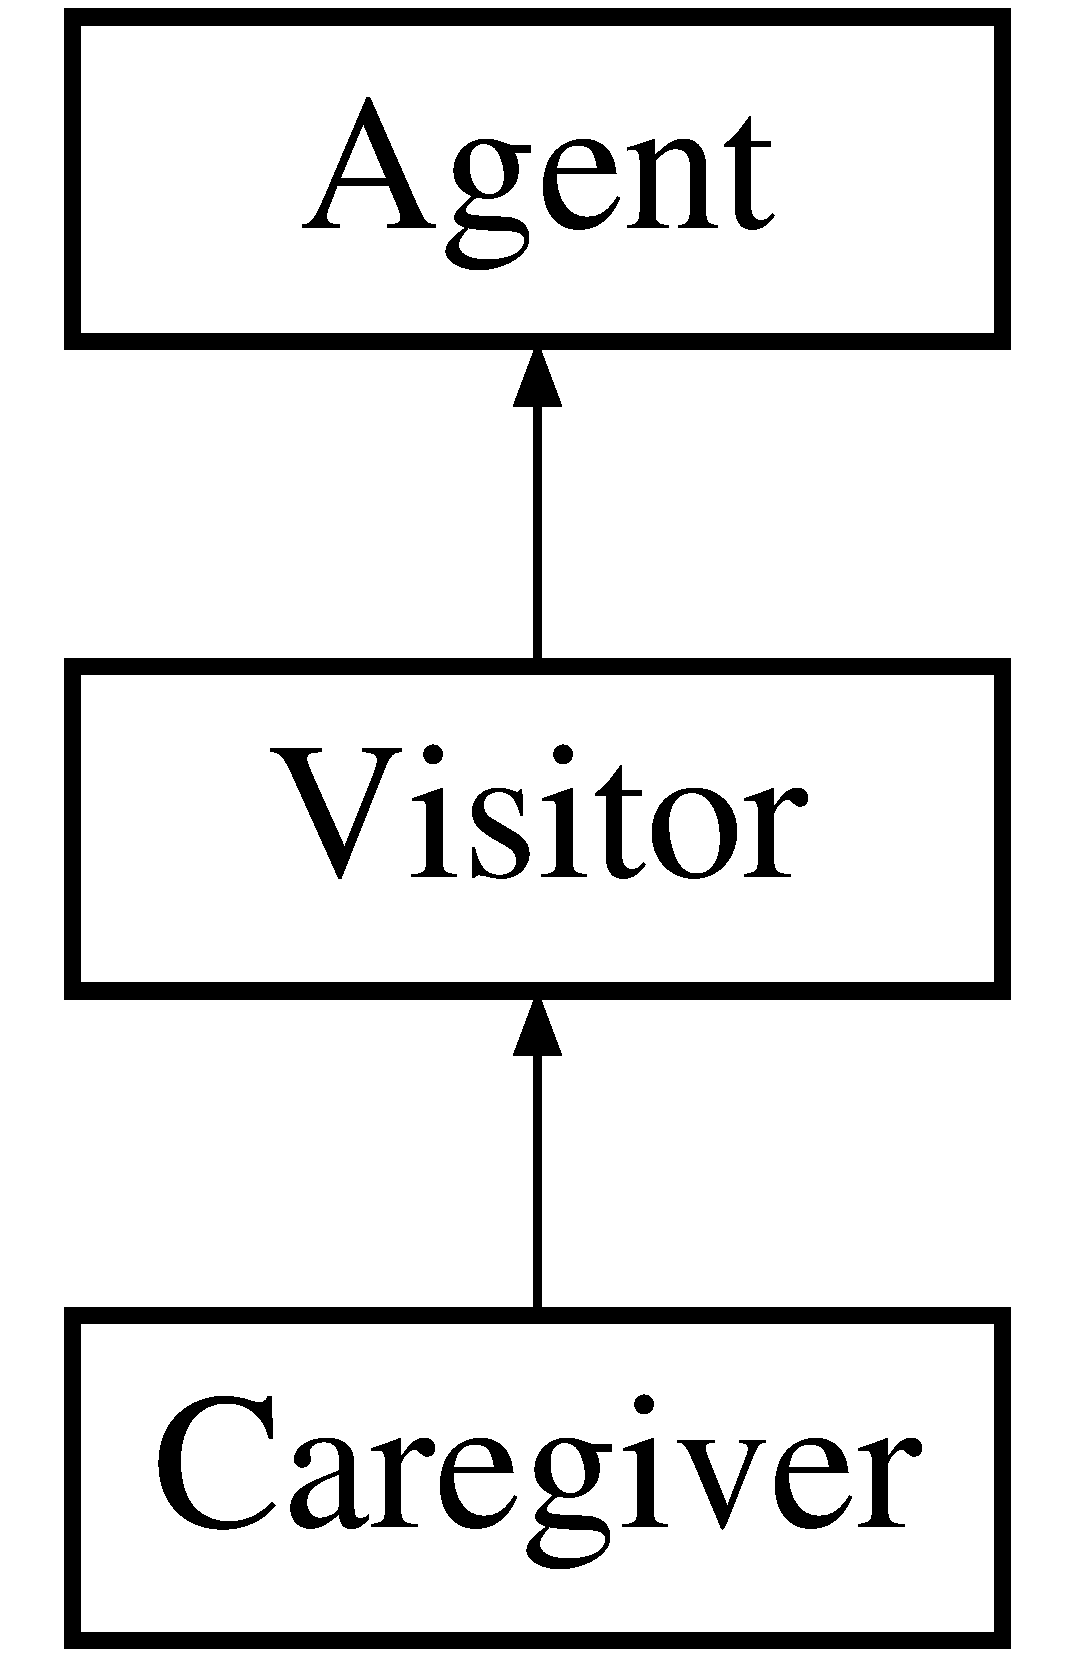
\includegraphics[height=3.000000cm]{classCaregiver}
\end{center}
\end{figure}
\subsection*{Public Member Functions}
\begin{DoxyCompactItemize}
\item 
void \hyperlink{classCaregiver_aa326466c62614b84d6a750dc0e59fa48}{Stage\-Odom\-\_\-callback} (nav\-\_\-msgs\-::\-Odometry msg)
\begin{DoxyCompactList}\small\item\em Updates the \hyperlink{classCaregiver}{Caregiver}'s x position, y position, and angle to reflect its current pose. \end{DoxyCompactList}\item 
void \hyperlink{classCaregiver_a3dc0edd8065745e6f355f80f2b293ba1}{Stage\-Laser\-\_\-callback} (sensor\-\_\-msgs\-::\-Laser\-Scan msg)
\begin{DoxyCompactList}\small\item\em Callback function to process laser scan messsages. You can access the range data from msg.\-ranges\mbox{[}i\mbox{]}. i = sample number. \end{DoxyCompactList}\item 
\hypertarget{classCaregiver_a8d1eccbe63af5842970daa69fedb40cc}{int \hyperlink{classCaregiver_a8d1eccbe63af5842970daa69fedb40cc}{run} (int argc, char $\ast$argv\mbox{[}$\,$\mbox{]})}\label{classCaregiver_a8d1eccbe63af5842970daa69fedb40cc}

\begin{DoxyCompactList}\small\item\em Main function for the \hyperlink{classCaregiver}{Caregiver} process. Controls node setup and periodic events. \end{DoxyCompactList}\end{DoxyCompactItemize}
\subsection*{Additional Inherited Members}


\subsection{Detailed Description}
Superclass for visitors -\/ i.\-e. Caregivers, Nurses, Doctors, Friends, Relatives. 

\subsection{Member Function Documentation}
\hypertarget{classCaregiver_a3dc0edd8065745e6f355f80f2b293ba1}{\index{Caregiver@{Caregiver}!Stage\-Laser\-\_\-callback@{Stage\-Laser\-\_\-callback}}
\index{Stage\-Laser\-\_\-callback@{Stage\-Laser\-\_\-callback}!Caregiver@{Caregiver}}
\subsubsection[{Stage\-Laser\-\_\-callback}]{\setlength{\rightskip}{0pt plus 5cm}void Caregiver\-::\-Stage\-Laser\-\_\-callback (
\begin{DoxyParamCaption}
\item[{sensor\-\_\-msgs\-::\-Laser\-Scan}]{msg}
\end{DoxyParamCaption}
)\hspace{0.3cm}{\ttfamily [virtual]}}}\label{classCaregiver_a3dc0edd8065745e6f355f80f2b293ba1}


Callback function to process laser scan messsages. You can access the range data from msg.\-ranges\mbox{[}i\mbox{]}. i = sample number. 

\begin{DoxyNote}{Note}
Currently blank as it is not in use. Navigation operates through a checkpoint system. 
\end{DoxyNote}

\begin{DoxyParams}{Parameters}
{\em msg} & Single scan from a planar laser range finder \\
\hline
\end{DoxyParams}


Implements \hyperlink{classAgent_adfe1de8bbeaa7e4a5f7f2ff3e45593e8}{Agent}.

\hypertarget{classCaregiver_aa326466c62614b84d6a750dc0e59fa48}{\index{Caregiver@{Caregiver}!Stage\-Odom\-\_\-callback@{Stage\-Odom\-\_\-callback}}
\index{Stage\-Odom\-\_\-callback@{Stage\-Odom\-\_\-callback}!Caregiver@{Caregiver}}
\subsubsection[{Stage\-Odom\-\_\-callback}]{\setlength{\rightskip}{0pt plus 5cm}void Caregiver\-::\-Stage\-Odom\-\_\-callback (
\begin{DoxyParamCaption}
\item[{nav\-\_\-msgs\-::\-Odometry}]{msg}
\end{DoxyParamCaption}
)\hspace{0.3cm}{\ttfamily [virtual]}}}\label{classCaregiver_aa326466c62614b84d6a750dc0e59fa48}


Updates the \hyperlink{classCaregiver}{Caregiver}'s x position, y position, and angle to reflect its current pose. 

\begin{DoxyNote}{Note}
Rounding is used to calculate the current angle. This approximation is accounted for by using threshholds when processing angles. 
\end{DoxyNote}

\begin{DoxyParams}{Parameters}
{\em msg} & Odometry message from odom topic \\
\hline
\end{DoxyParams}


Implements \hyperlink{classAgent_a4b1182b9ee5dccaa871d71beef94a7d2}{Agent}.



The documentation for this class was generated from the following files\-:\begin{DoxyCompactItemize}
\item 
se306\-\_\-project1/src/Caregiver.\-h\item 
se306\-\_\-project1/src/Caregiver.\-cpp\end{DoxyCompactItemize}

\hypertarget{classCaregiver1}{\section{Caregiver1 Class Reference}
\label{classCaregiver1}\index{Caregiver1@{Caregiver1}}
}


Superclass for visitors -\/ i.\-e. Caregivers, Nurses, Doctors, Friends, Relatives.  




{\ttfamily \#include $<$Caregiver1.\-h$>$}

Inheritance diagram for Caregiver1\-:\begin{figure}[H]
\begin{center}
\leavevmode
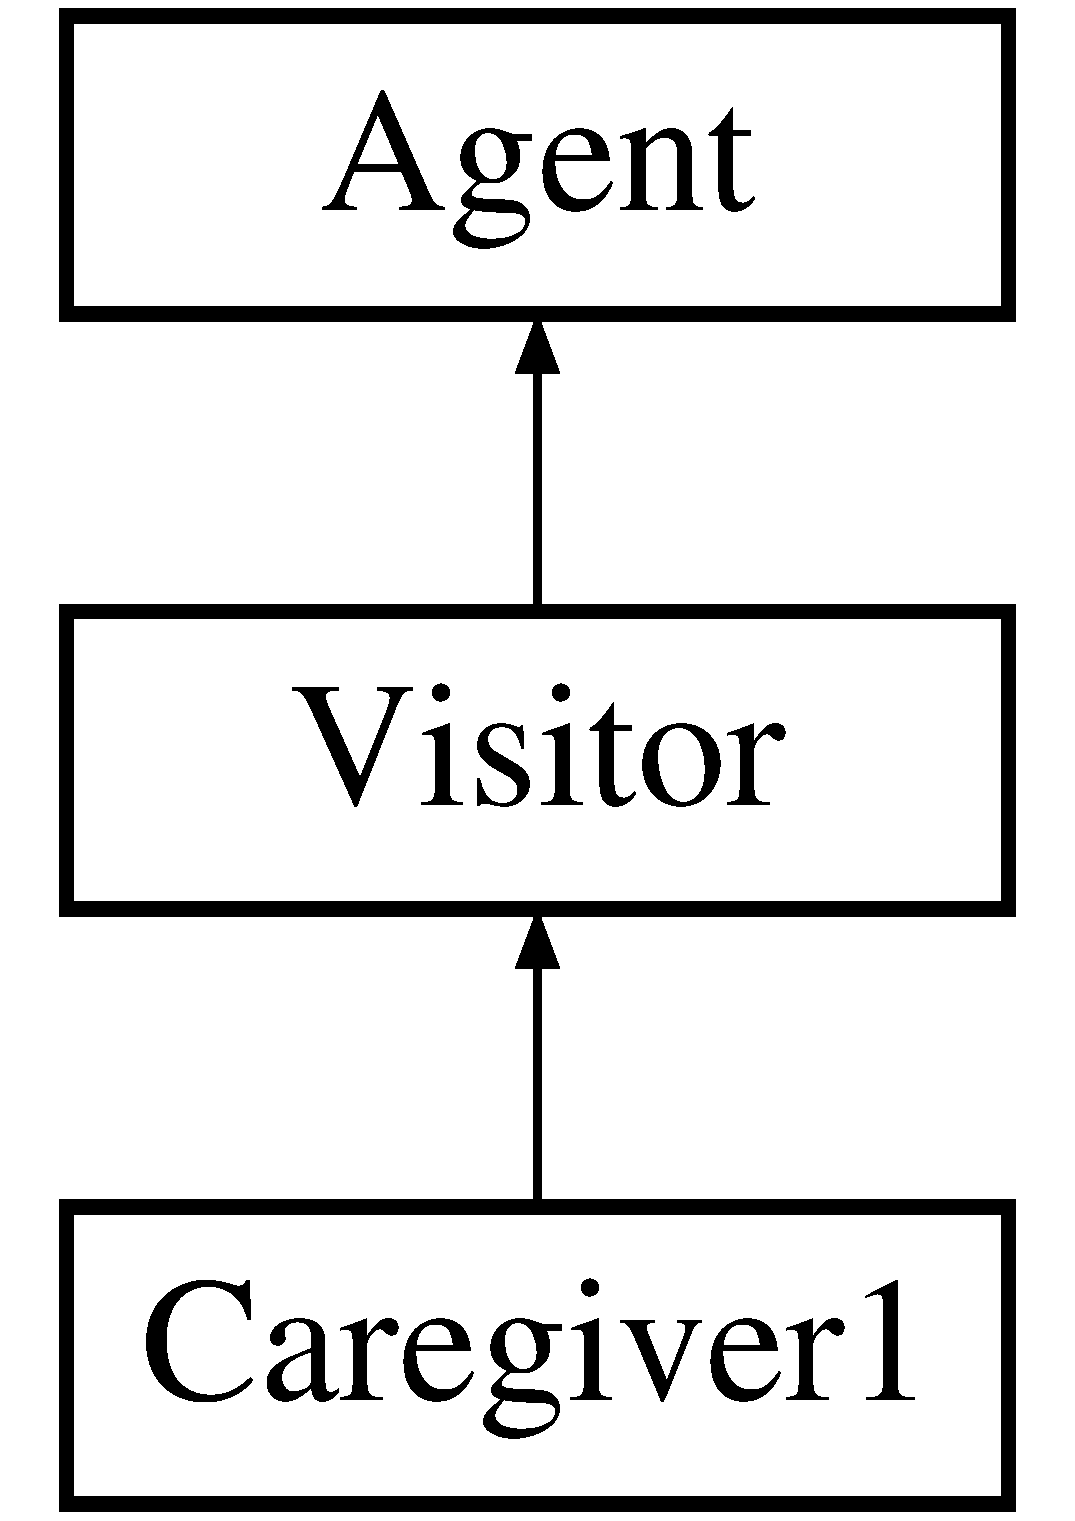
\includegraphics[height=3.000000cm]{classCaregiver1}
\end{center}
\end{figure}
\subsection*{Public Member Functions}
\begin{DoxyCompactItemize}
\item 
\hypertarget{classCaregiver1_a71affa8e6bfe53f238ab3ca27dbdab6a}{int \hyperlink{classCaregiver1_a71affa8e6bfe53f238ab3ca27dbdab6a}{run} (int argc, char $\ast$argv\mbox{[}$\,$\mbox{]})}\label{classCaregiver1_a71affa8e6bfe53f238ab3ca27dbdab6a}

\begin{DoxyCompactList}\small\item\em Main function for the \hyperlink{classCaregiver}{Caregiver} process. Controls node setup and periodic events. \end{DoxyCompactList}\end{DoxyCompactItemize}
\subsection*{Additional Inherited Members}


\subsection{Detailed Description}
Superclass for visitors -\/ i.\-e. Caregivers, Nurses, Doctors, Friends, Relatives. 

The documentation for this class was generated from the following files\-:\begin{DoxyCompactItemize}
\item 
se306\-\_\-project1/src/Caregiver1.\-h\item 
se306\-\_\-project1/src/Caregiver1.\-cpp\end{DoxyCompactItemize}

\hypertarget{classCaregiver2}{\section{Caregiver2 Class Reference}
\label{classCaregiver2}\index{Caregiver2@{Caregiver2}}
}


Superclass for visitors -\/ i.\-e. Caregivers, Nurses, Doctors, Friends, Relatives.  




{\ttfamily \#include $<$Caregiver2.\-h$>$}

Inheritance diagram for Caregiver2\-:\begin{figure}[H]
\begin{center}
\leavevmode
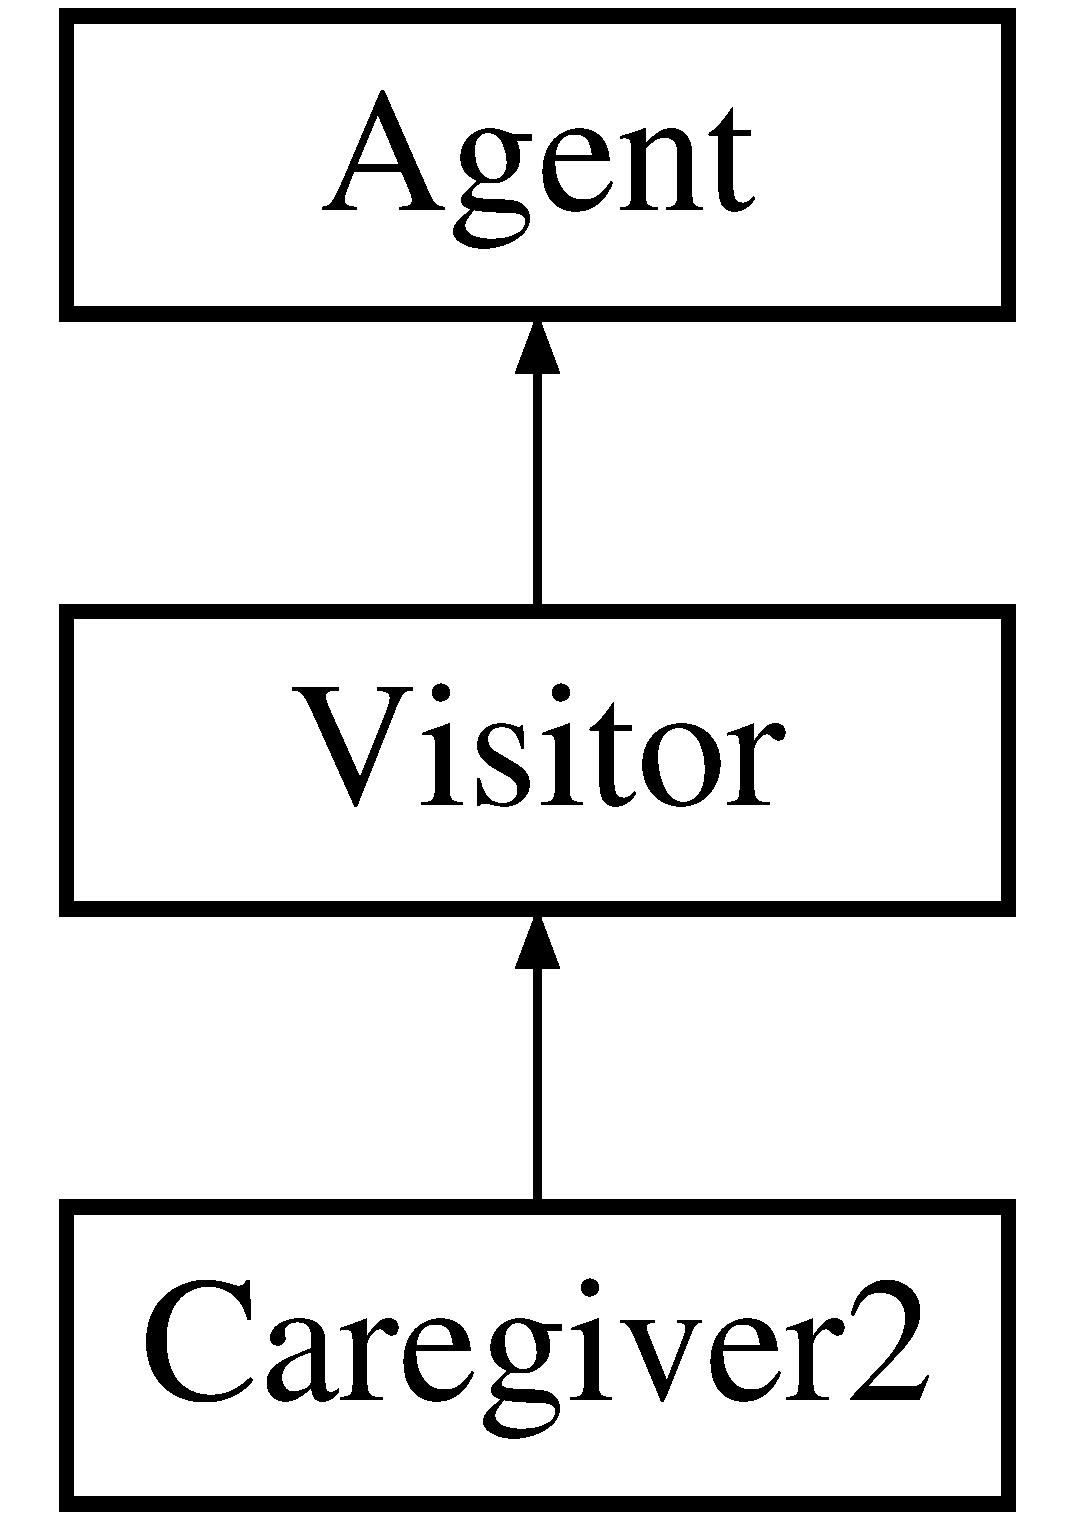
\includegraphics[height=3.000000cm]{classCaregiver2}
\end{center}
\end{figure}
\subsection*{Public Member Functions}
\begin{DoxyCompactItemize}
\item 
\hypertarget{classCaregiver2_a65af1d2308e093124b79c53ba43120d3}{int \hyperlink{classCaregiver2_a65af1d2308e093124b79c53ba43120d3}{run} (int argc, char $\ast$argv\mbox{[}$\,$\mbox{]})}\label{classCaregiver2_a65af1d2308e093124b79c53ba43120d3}

\begin{DoxyCompactList}\small\item\em Main function for the \hyperlink{classCaregiver}{Caregiver} process. Controls node setup and periodic events. \end{DoxyCompactList}\end{DoxyCompactItemize}
\subsection*{Additional Inherited Members}


\subsection{Detailed Description}
Superclass for visitors -\/ i.\-e. Caregivers, Nurses, Doctors, Friends, Relatives. 

The documentation for this class was generated from the following files\-:\begin{DoxyCompactItemize}
\item 
se306\-\_\-project1/src/Caregiver2.\-h\item 
se306\-\_\-project1/src/Caregiver2.\-cpp\end{DoxyCompactItemize}

\hypertarget{classCheckPointGraph}{\section{Check\-Point\-Graph Class Reference}
\label{classCheckPointGraph}\index{Check\-Point\-Graph@{Check\-Point\-Graph}}
}
\subsection*{Public Member Functions}
\begin{DoxyCompactItemize}
\item 
\hypertarget{classCheckPointGraph_a417bcd9db81360b38575569f3900b0c0}{void \hyperlink{classCheckPointGraph_a417bcd9db81360b38575569f3900b0c0}{make\-Graph} ()}\label{classCheckPointGraph_a417bcd9db81360b38575569f3900b0c0}

\begin{DoxyCompactList}\small\item\em Creates a graph of checkpoint names, provided the vector of names and the array of edges. Uses boost's adjacency list. \end{DoxyCompactList}\item 
\hypertarget{classCheckPointGraph_a07e2e7cf2afa95d82076f87600761728}{void \hyperlink{classCheckPointGraph_a07e2e7cf2afa95d82076f87600761728}{checkpoint\-Map} ()}\label{classCheckPointGraph_a07e2e7cf2afa95d82076f87600761728}

\begin{DoxyCompactList}\small\item\em Associates checkpoint names with checkpoint co-\/ordinates To be used in conjunction with a graph of checkpoint names, representing paths between checkpoints. Could be replaced by adding the co-\/ordinates to bundled properties in the property map of the graph. \end{DoxyCompactList}\item 
std\-::vector$<$ std\-::pair$<$ double, \\*
double $>$ $>$ \hyperlink{classCheckPointGraph_ab48dfe7feccab1d732901b83a0ec4612}{shortest\-Path} (std\-::string start\-Name, std\-::string end\-Name)
\begin{DoxyCompactList}\small\item\em Finds the shortest path between 2 checkpoints, and returns the path as co-\/ordinates. Uses breadth first search -\/ Boost recommends this over Dijkstra's algorithm for graphs with uniformly weighted edges. Sets path member variable. \end{DoxyCompactList}\item 
\hypertarget{classCheckPointGraph_a92da1b78dfbf86627397265c43143100}{std\-::string {\bfseries get\-Checkpoint\-Name} (std\-::pair$<$ double, double $>$ coords)}\label{classCheckPointGraph_a92da1b78dfbf86627397265c43143100}

\item 
\hypertarget{classCheckPointGraph_a2200216c4d24426b2b479b3a8bb7141d}{std\-::pair$<$ double, double $>$ {\bfseries get\-Coords} (std\-::string name)}\label{classCheckPointGraph_a2200216c4d24426b2b479b3a8bb7141d}

\end{DoxyCompactItemize}


\subsection{Member Function Documentation}
\hypertarget{classCheckPointGraph_ab48dfe7feccab1d732901b83a0ec4612}{\index{Check\-Point\-Graph@{Check\-Point\-Graph}!shortest\-Path@{shortest\-Path}}
\index{shortest\-Path@{shortest\-Path}!CheckPointGraph@{Check\-Point\-Graph}}
\subsubsection[{shortest\-Path}]{\setlength{\rightskip}{0pt plus 5cm}std\-::vector$<$ std\-::pair$<$ double, double $>$ $>$ Check\-Point\-Graph\-::shortest\-Path (
\begin{DoxyParamCaption}
\item[{std\-::string}]{start\-Name, }
\item[{std\-::string}]{end\-Name}
\end{DoxyParamCaption}
)}}\label{classCheckPointGraph_ab48dfe7feccab1d732901b83a0ec4612}


Finds the shortest path between 2 checkpoints, and returns the path as co-\/ordinates. Uses breadth first search -\/ Boost recommends this over Dijkstra's algorithm for graphs with uniformly weighted edges. Sets path member variable. 


\begin{DoxyParams}{Parameters}
{\em start\-Name} & The name of the start checkpoint as a string (e.\-g. 'kitchen') \\
\hline
{\em end\-Name} & The name of the goal checkpoint as a string (e.\-g. 'bathroom') \\
\hline
\end{DoxyParams}


The documentation for this class was generated from the following files\-:\begin{DoxyCompactItemize}
\item 
se306\-\_\-project1/src/Check\-Point\-Graph.\-hpp\item 
se306\-\_\-project1/src/Check\-Point\-Graph.\-cpp\end{DoxyCompactItemize}

\hypertarget{structros_1_1message__traits_1_1DataType_3_01_1_1se306__project1_1_1AssistantMsg___3_01ContainerAllocator_01_4_01_4}{\section{ros\-:\-:message\-\_\-traits\-:\-:Data\-Type$<$ \-:\-:se306\-\_\-project1\-:\-:Assistant\-Msg\-\_\-$<$ Container\-Allocator $>$ $>$ Struct Template Reference}
\label{structros_1_1message__traits_1_1DataType_3_01_1_1se306__project1_1_1AssistantMsg___3_01ContainerAllocator_01_4_01_4}\index{ros\-::message\-\_\-traits\-::\-Data\-Type$<$ \-::se306\-\_\-project1\-::\-Assistant\-Msg\-\_\-$<$ Container\-Allocator $>$ $>$@{ros\-::message\-\_\-traits\-::\-Data\-Type$<$ \-::se306\-\_\-project1\-::\-Assistant\-Msg\-\_\-$<$ Container\-Allocator $>$ $>$}}
}
\subsection*{Static Public Member Functions}
\begin{DoxyCompactItemize}
\item 
\hypertarget{structros_1_1message__traits_1_1DataType_3_01_1_1se306__project1_1_1AssistantMsg___3_01ContainerAllocator_01_4_01_4_ae0a879b4dd29f9b66a0d0f1ea073a641}{static const char $\ast$ {\bfseries value} ()}\label{structros_1_1message__traits_1_1DataType_3_01_1_1se306__project1_1_1AssistantMsg___3_01ContainerAllocator_01_4_01_4_ae0a879b4dd29f9b66a0d0f1ea073a641}

\item 
\hypertarget{structros_1_1message__traits_1_1DataType_3_01_1_1se306__project1_1_1AssistantMsg___3_01ContainerAllocator_01_4_01_4_ad7010538055bae2cac07b2f8192b4bc1}{static const char $\ast$ {\bfseries value} (const \-::\hyperlink{structse306__project1_1_1AssistantMsg__}{se306\-\_\-project1\-::\-Assistant\-Msg\-\_\-}$<$ Container\-Allocator $>$ \&)}\label{structros_1_1message__traits_1_1DataType_3_01_1_1se306__project1_1_1AssistantMsg___3_01ContainerAllocator_01_4_01_4_ad7010538055bae2cac07b2f8192b4bc1}

\end{DoxyCompactItemize}


The documentation for this struct was generated from the following file\-:\begin{DoxyCompactItemize}
\item 
se306\-\_\-project1/msg\-\_\-gen/cpp/include/se306\-\_\-project1/Assistant\-Msg.\-h\end{DoxyCompactItemize}

\hypertarget{structros_1_1message__traits_1_1DataType_3_01_1_1se306__project1_1_1DoctorMsg___3_01ContainerAllocator_01_4_01_4}{\section{ros\-:\-:message\-\_\-traits\-:\-:Data\-Type$<$ \-:\-:se306\-\_\-project1\-:\-:Doctor\-Msg\-\_\-$<$ Container\-Allocator $>$ $>$ Struct Template Reference}
\label{structros_1_1message__traits_1_1DataType_3_01_1_1se306__project1_1_1DoctorMsg___3_01ContainerAllocator_01_4_01_4}\index{ros\-::message\-\_\-traits\-::\-Data\-Type$<$ \-::se306\-\_\-project1\-::\-Doctor\-Msg\-\_\-$<$ Container\-Allocator $>$ $>$@{ros\-::message\-\_\-traits\-::\-Data\-Type$<$ \-::se306\-\_\-project1\-::\-Doctor\-Msg\-\_\-$<$ Container\-Allocator $>$ $>$}}
}
\subsection*{Static Public Member Functions}
\begin{DoxyCompactItemize}
\item 
\hypertarget{structros_1_1message__traits_1_1DataType_3_01_1_1se306__project1_1_1DoctorMsg___3_01ContainerAllocator_01_4_01_4_ad3eea037c0d845107620384a6a188ed0}{static const char $\ast$ {\bfseries value} ()}\label{structros_1_1message__traits_1_1DataType_3_01_1_1se306__project1_1_1DoctorMsg___3_01ContainerAllocator_01_4_01_4_ad3eea037c0d845107620384a6a188ed0}

\item 
\hypertarget{structros_1_1message__traits_1_1DataType_3_01_1_1se306__project1_1_1DoctorMsg___3_01ContainerAllocator_01_4_01_4_ab08d23c5013ac40731f32b595e825e5b}{static const char $\ast$ {\bfseries value} (const \-::\hyperlink{structse306__project1_1_1DoctorMsg__}{se306\-\_\-project1\-::\-Doctor\-Msg\-\_\-}$<$ Container\-Allocator $>$ \&)}\label{structros_1_1message__traits_1_1DataType_3_01_1_1se306__project1_1_1DoctorMsg___3_01ContainerAllocator_01_4_01_4_ab08d23c5013ac40731f32b595e825e5b}

\end{DoxyCompactItemize}


The documentation for this struct was generated from the following file\-:\begin{DoxyCompactItemize}
\item 
se306\-\_\-project1/msg\-\_\-gen/cpp/include/se306\-\_\-project1/Doctor\-Msg.\-h\end{DoxyCompactItemize}

\hypertarget{structros_1_1message__traits_1_1DataType_3_01_1_1se306__project1_1_1ResidentMsg___3_01ContainerAllocator_01_4_01_4}{\section{ros\-:\-:message\-\_\-traits\-:\-:Data\-Type$<$ \-:\-:se306\-\_\-project1\-:\-:Resident\-Msg\-\_\-$<$ Container\-Allocator $>$ $>$ Struct Template Reference}
\label{structros_1_1message__traits_1_1DataType_3_01_1_1se306__project1_1_1ResidentMsg___3_01ContainerAllocator_01_4_01_4}\index{ros\-::message\-\_\-traits\-::\-Data\-Type$<$ \-::se306\-\_\-project1\-::\-Resident\-Msg\-\_\-$<$ Container\-Allocator $>$ $>$@{ros\-::message\-\_\-traits\-::\-Data\-Type$<$ \-::se306\-\_\-project1\-::\-Resident\-Msg\-\_\-$<$ Container\-Allocator $>$ $>$}}
}
\subsection*{Static Public Member Functions}
\begin{DoxyCompactItemize}
\item 
\hypertarget{structros_1_1message__traits_1_1DataType_3_01_1_1se306__project1_1_1ResidentMsg___3_01ContainerAllocator_01_4_01_4_a9a31b5a0b94c41142bca37e8a17083af}{static const char $\ast$ {\bfseries value} ()}\label{structros_1_1message__traits_1_1DataType_3_01_1_1se306__project1_1_1ResidentMsg___3_01ContainerAllocator_01_4_01_4_a9a31b5a0b94c41142bca37e8a17083af}

\item 
\hypertarget{structros_1_1message__traits_1_1DataType_3_01_1_1se306__project1_1_1ResidentMsg___3_01ContainerAllocator_01_4_01_4_a0a4c15240b3a040bd06d02e53a1ae6fd}{static const char $\ast$ {\bfseries value} (const \-::\hyperlink{structse306__project1_1_1ResidentMsg__}{se306\-\_\-project1\-::\-Resident\-Msg\-\_\-}$<$ Container\-Allocator $>$ \&)}\label{structros_1_1message__traits_1_1DataType_3_01_1_1se306__project1_1_1ResidentMsg___3_01ContainerAllocator_01_4_01_4_a0a4c15240b3a040bd06d02e53a1ae6fd}

\end{DoxyCompactItemize}


The documentation for this struct was generated from the following file\-:\begin{DoxyCompactItemize}
\item 
se306\-\_\-project1/msg\-\_\-gen/cpp/include/se306\-\_\-project1/Resident\-Msg.\-h\end{DoxyCompactItemize}

\hypertarget{structros_1_1message__traits_1_1Definition_3_01_1_1se306__project1_1_1AssistantMsg___3_01ContainerAllocator_01_4_01_4}{\section{ros\-:\-:message\-\_\-traits\-:\-:Definition$<$ \-:\-:se306\-\_\-project1\-:\-:Assistant\-Msg\-\_\-$<$ Container\-Allocator $>$ $>$ Struct Template Reference}
\label{structros_1_1message__traits_1_1Definition_3_01_1_1se306__project1_1_1AssistantMsg___3_01ContainerAllocator_01_4_01_4}\index{ros\-::message\-\_\-traits\-::\-Definition$<$ \-::se306\-\_\-project1\-::\-Assistant\-Msg\-\_\-$<$ Container\-Allocator $>$ $>$@{ros\-::message\-\_\-traits\-::\-Definition$<$ \-::se306\-\_\-project1\-::\-Assistant\-Msg\-\_\-$<$ Container\-Allocator $>$ $>$}}
}
\subsection*{Static Public Member Functions}
\begin{DoxyCompactItemize}
\item 
\hypertarget{structros_1_1message__traits_1_1Definition_3_01_1_1se306__project1_1_1AssistantMsg___3_01ContainerAllocator_01_4_01_4_a9ca6b367a578a8e9dc084ed7aa46a23d}{static const char $\ast$ {\bfseries value} ()}\label{structros_1_1message__traits_1_1Definition_3_01_1_1se306__project1_1_1AssistantMsg___3_01ContainerAllocator_01_4_01_4_a9ca6b367a578a8e9dc084ed7aa46a23d}

\item 
\hypertarget{structros_1_1message__traits_1_1Definition_3_01_1_1se306__project1_1_1AssistantMsg___3_01ContainerAllocator_01_4_01_4_a71ca5d6aa141f74243f51a0d8f68ec8f}{static const char $\ast$ {\bfseries value} (const \-::\hyperlink{structse306__project1_1_1AssistantMsg__}{se306\-\_\-project1\-::\-Assistant\-Msg\-\_\-}$<$ Container\-Allocator $>$ \&)}\label{structros_1_1message__traits_1_1Definition_3_01_1_1se306__project1_1_1AssistantMsg___3_01ContainerAllocator_01_4_01_4_a71ca5d6aa141f74243f51a0d8f68ec8f}

\end{DoxyCompactItemize}


The documentation for this struct was generated from the following file\-:\begin{DoxyCompactItemize}
\item 
se306\-\_\-project1/msg\-\_\-gen/cpp/include/se306\-\_\-project1/Assistant\-Msg.\-h\end{DoxyCompactItemize}

\hypertarget{structros_1_1message__traits_1_1Definition_3_01_1_1se306__project1_1_1DoctorMsg___3_01ContainerAllocator_01_4_01_4}{\section{ros\-:\-:message\-\_\-traits\-:\-:Definition$<$ \-:\-:se306\-\_\-project1\-:\-:Doctor\-Msg\-\_\-$<$ Container\-Allocator $>$ $>$ Struct Template Reference}
\label{structros_1_1message__traits_1_1Definition_3_01_1_1se306__project1_1_1DoctorMsg___3_01ContainerAllocator_01_4_01_4}\index{ros\-::message\-\_\-traits\-::\-Definition$<$ \-::se306\-\_\-project1\-::\-Doctor\-Msg\-\_\-$<$ Container\-Allocator $>$ $>$@{ros\-::message\-\_\-traits\-::\-Definition$<$ \-::se306\-\_\-project1\-::\-Doctor\-Msg\-\_\-$<$ Container\-Allocator $>$ $>$}}
}
\subsection*{Static Public Member Functions}
\begin{DoxyCompactItemize}
\item 
\hypertarget{structros_1_1message__traits_1_1Definition_3_01_1_1se306__project1_1_1DoctorMsg___3_01ContainerAllocator_01_4_01_4_ada7e90b274706a782c74d5aa408f9d64}{static const char $\ast$ {\bfseries value} ()}\label{structros_1_1message__traits_1_1Definition_3_01_1_1se306__project1_1_1DoctorMsg___3_01ContainerAllocator_01_4_01_4_ada7e90b274706a782c74d5aa408f9d64}

\item 
\hypertarget{structros_1_1message__traits_1_1Definition_3_01_1_1se306__project1_1_1DoctorMsg___3_01ContainerAllocator_01_4_01_4_ab123a047e7407f9d9ba2c29267f63ab7}{static const char $\ast$ {\bfseries value} (const \-::\hyperlink{structse306__project1_1_1DoctorMsg__}{se306\-\_\-project1\-::\-Doctor\-Msg\-\_\-}$<$ Container\-Allocator $>$ \&)}\label{structros_1_1message__traits_1_1Definition_3_01_1_1se306__project1_1_1DoctorMsg___3_01ContainerAllocator_01_4_01_4_ab123a047e7407f9d9ba2c29267f63ab7}

\end{DoxyCompactItemize}


The documentation for this struct was generated from the following file\-:\begin{DoxyCompactItemize}
\item 
se306\-\_\-project1/msg\-\_\-gen/cpp/include/se306\-\_\-project1/Doctor\-Msg.\-h\end{DoxyCompactItemize}

\hypertarget{structros_1_1message__traits_1_1Definition_3_01_1_1se306__project1_1_1ResidentMsg___3_01ContainerAllocator_01_4_01_4}{\section{ros\-:\-:message\-\_\-traits\-:\-:Definition$<$ \-:\-:se306\-\_\-project1\-:\-:Resident\-Msg\-\_\-$<$ Container\-Allocator $>$ $>$ Struct Template Reference}
\label{structros_1_1message__traits_1_1Definition_3_01_1_1se306__project1_1_1ResidentMsg___3_01ContainerAllocator_01_4_01_4}\index{ros\-::message\-\_\-traits\-::\-Definition$<$ \-::se306\-\_\-project1\-::\-Resident\-Msg\-\_\-$<$ Container\-Allocator $>$ $>$@{ros\-::message\-\_\-traits\-::\-Definition$<$ \-::se306\-\_\-project1\-::\-Resident\-Msg\-\_\-$<$ Container\-Allocator $>$ $>$}}
}
\subsection*{Static Public Member Functions}
\begin{DoxyCompactItemize}
\item 
\hypertarget{structros_1_1message__traits_1_1Definition_3_01_1_1se306__project1_1_1ResidentMsg___3_01ContainerAllocator_01_4_01_4_a7456e6595722ccfcad34cb29b1c76d2b}{static const char $\ast$ {\bfseries value} ()}\label{structros_1_1message__traits_1_1Definition_3_01_1_1se306__project1_1_1ResidentMsg___3_01ContainerAllocator_01_4_01_4_a7456e6595722ccfcad34cb29b1c76d2b}

\item 
\hypertarget{structros_1_1message__traits_1_1Definition_3_01_1_1se306__project1_1_1ResidentMsg___3_01ContainerAllocator_01_4_01_4_a9036589abcf9b2afa910914cac0d57a8}{static const char $\ast$ {\bfseries value} (const \-::\hyperlink{structse306__project1_1_1ResidentMsg__}{se306\-\_\-project1\-::\-Resident\-Msg\-\_\-}$<$ Container\-Allocator $>$ \&)}\label{structros_1_1message__traits_1_1Definition_3_01_1_1se306__project1_1_1ResidentMsg___3_01ContainerAllocator_01_4_01_4_a9036589abcf9b2afa910914cac0d57a8}

\end{DoxyCompactItemize}


The documentation for this struct was generated from the following file\-:\begin{DoxyCompactItemize}
\item 
se306\-\_\-project1/msg\-\_\-gen/cpp/include/se306\-\_\-project1/Resident\-Msg.\-h\end{DoxyCompactItemize}

\hypertarget{classDoctor}{\section{Doctor Class Reference}
\label{classDoctor}\index{Doctor@{Doctor}}
}
Inheritance diagram for Doctor\-:\begin{figure}[H]
\begin{center}
\leavevmode
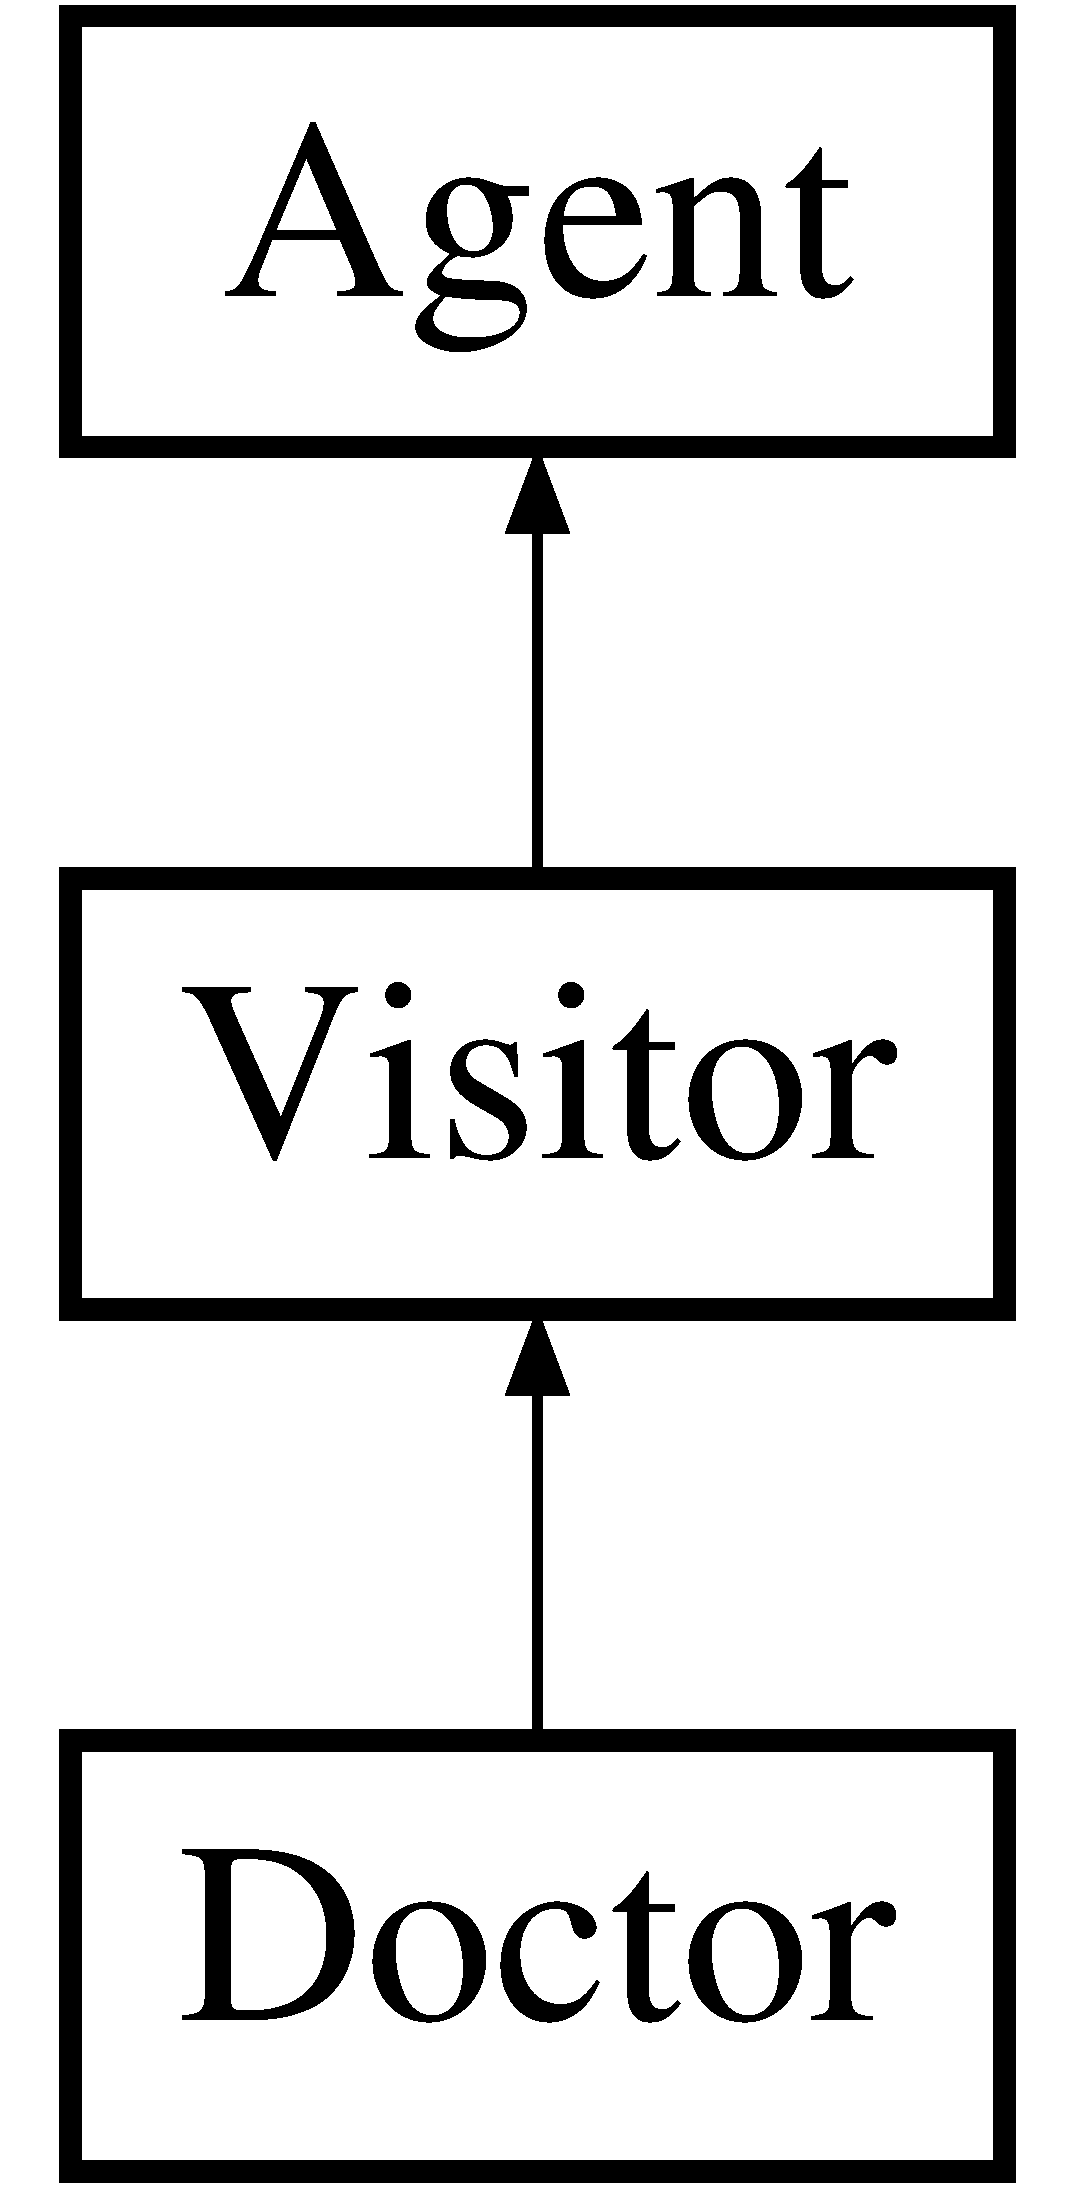
\includegraphics[height=3.000000cm]{classDoctor}
\end{center}
\end{figure}
\subsection*{Public Member Functions}
\begin{DoxyCompactItemize}
\item 
\hypertarget{classDoctor_a92b20f52198c6137d8858152cba77640}{void {\bfseries Stage\-Odom\-\_\-callback} (nav\-\_\-msgs\-::\-Odometry msg)}\label{classDoctor_a92b20f52198c6137d8858152cba77640}

\item 
\hypertarget{classDoctor_ab0b46ba92bd2069733f304858b7e4495}{void {\bfseries Stage\-Laser\-\_\-callback} (sensor\-\_\-msgs\-::\-Laser\-Scan msg)}\label{classDoctor_ab0b46ba92bd2069733f304858b7e4495}

\item 
\hypertarget{classDoctor_a1fe9c9a74bd4d2044b7217ec82ae9e60}{int {\bfseries run} (int argc, char $\ast$$\ast$argv)}\label{classDoctor_a1fe9c9a74bd4d2044b7217ec82ae9e60}

\item 
\hypertarget{classDoctor_a55fe6c06a3ce07fd9014a03000df43db}{double {\bfseries calc\-\_\-goal\-\_\-angle} (double goal\-\_\-x, double goal\-\_\-y, double cur\-\_\-angle, double px, double py)}\label{classDoctor_a55fe6c06a3ce07fd9014a03000df43db}

\item 
\hypertarget{classDoctor_ada60bb6625be46966ff86f7af9d05366}{std\-::pair$<$ double, double $>$ {\bfseries move} (double goal\-\_\-x, double goal\-\_\-y, double cur\-\_\-angle, double goal\-\_\-angle, double px, double py)}\label{classDoctor_ada60bb6625be46966ff86f7af9d05366}

\item 
\hypertarget{classDoctor_a21ac6188dd7f5890ff1a633cf700144d}{void {\bfseries random\-Checkpoint\-Callback} (const ros\-::\-Timer\-Event \&)}\label{classDoctor_a21ac6188dd7f5890ff1a633cf700144d}

\item 
\hypertarget{classDoctor_aed76815aa67aec25e8ff86a55e4ac4f1}{std\-::pair$<$ double, double $>$ {\bfseries move\-Path} (int path\mbox{[}$\,$\mbox{]}\mbox{[}2\mbox{]}, int path\-Length)}\label{classDoctor_aed76815aa67aec25e8ff86a55e4ac4f1}

\item 
\hypertarget{classDoctor_af4d24247a3f59b1b3b5258938e019086}{void {\bfseries resident\-Status\-Callback} (\hyperlink{structse306__project1_1_1ResidentMsg__}{se306\-\_\-project1\-::\-Resident\-Msg} msg)}\label{classDoctor_af4d24247a3f59b1b3b5258938e019086}

\item 
\hypertarget{classDoctor_a26ae14986239ea67147a52235685e31e}{void {\bfseries medication\-Callback} (const ros\-::\-Timer\-Event \&)}\label{classDoctor_a26ae14986239ea67147a52235685e31e}

\end{DoxyCompactItemize}
\subsection*{Protected Attributes}
\begin{DoxyCompactItemize}
\item 
\hypertarget{classDoctor_adab6ec6a93ee2f58b436a8294120f295}{bool {\bfseries heal\-Resident}}\label{classDoctor_adab6ec6a93ee2f58b436a8294120f295}

\item 
\hypertarget{classDoctor_ab1814310e306e7a742ffa9c5c6b913ef}{int {\bfseries health}}\label{classDoctor_ab1814310e306e7a742ffa9c5c6b913ef}

\item 
\hypertarget{classDoctor_a76dcb7e1308ef8001b7960cb542e3824}{int {\bfseries boredom}}\label{classDoctor_a76dcb7e1308ef8001b7960cb542e3824}

\item 
\hypertarget{classDoctor_a7b59e97eb09eed2ffed797d1174ac47f}{int {\bfseries hunger}}\label{classDoctor_a7b59e97eb09eed2ffed797d1174ac47f}

\item 
\hypertarget{classDoctor_ae058c3d6dce31d71ac4e63e3fd653275}{double {\bfseries goal\-\_\-x}}\label{classDoctor_ae058c3d6dce31d71ac4e63e3fd653275}

\item 
\hypertarget{classDoctor_aba0c1163551f144834fc0d68c556fac2}{double {\bfseries goal\-\_\-y}}\label{classDoctor_aba0c1163551f144834fc0d68c556fac2}

\item 
\hypertarget{classDoctor_a6ea729b1a8fc6d33176d768ef62b0a43}{double {\bfseries px}}\label{classDoctor_a6ea729b1a8fc6d33176d768ef62b0a43}

\item 
\hypertarget{classDoctor_a04b4b5bddd2b99b6eb4b7b8813eeeebf}{double {\bfseries py}}\label{classDoctor_a04b4b5bddd2b99b6eb4b7b8813eeeebf}

\item 
\hypertarget{classDoctor_a27377808d49670322af2ce4ec34730f1}{double {\bfseries goal\-\_\-angle}}\label{classDoctor_a27377808d49670322af2ce4ec34730f1}

\item 
\hypertarget{classDoctor_a2f7dffac0f8141914640e8f9bee5e7ff}{bool {\bfseries running}}\label{classDoctor_a2f7dffac0f8141914640e8f9bee5e7ff}

\item 
\hypertarget{classDoctor_ae31c0df1faec161bc8fec8dfae55b139}{bool {\bfseries is\-Set}}\label{classDoctor_ae31c0df1faec161bc8fec8dfae55b139}

\item 
\hypertarget{classDoctor_ab67e7a3eab1a57a0cfa52d84fe52414d}{double {\bfseries cur\-\_\-angle}}\label{classDoctor_ab67e7a3eab1a57a0cfa52d84fe52414d}

\item 
\hypertarget{classDoctor_a254303eb3ae4982340eb079ea76e942a}{int {\bfseries cc} = 1}\label{classDoctor_a254303eb3ae4982340eb079ea76e942a}

\item 
\hypertarget{classDoctor_a0566f795b41ece871b82ed7b63c5a780}{bool {\bfseries is\-\_\-called}}\label{classDoctor_a0566f795b41ece871b82ed7b63c5a780}

\item 
\hypertarget{classDoctor_a31d510c612a7f9d59efbcc8327f7adf3}{std\-::pair$<$ double, bool $>$ {\bfseries goal\-\_\-pair}}\label{classDoctor_a31d510c612a7f9d59efbcc8327f7adf3}

\item 
\hypertarget{classDoctor_ac371e75b4dcac584c9f2fa89585fefd7}{std\-::pair$<$ double, double $>$ {\bfseries ret}}\label{classDoctor_ac371e75b4dcac584c9f2fa89585fefd7}

\item 
int {\bfseries checkpoints} \mbox{[}4\mbox{]}\mbox{[}2\mbox{]}
\end{DoxyCompactItemize}
\subsection*{Additional Inherited Members}


\subsection{Member Data Documentation}
\hypertarget{classDoctor_a9bb025d7f8f843371b1c63414272afe1}{\index{Doctor@{Doctor}!checkpoints@{checkpoints}}
\index{checkpoints@{checkpoints}!Doctor@{Doctor}}
\subsubsection[{checkpoints}]{\setlength{\rightskip}{0pt plus 5cm}int Doctor\-::checkpoints\mbox{[}4\mbox{]}\mbox{[}2\mbox{]}\hspace{0.3cm}{\ttfamily [protected]}}}\label{classDoctor_a9bb025d7f8f843371b1c63414272afe1}
{\bfseries Initial value\-:}
\begin{DoxyCode}
= \{
                \{10, -7\},
                \{10, 2\},
                \{30, 20\},
                \{30, 25\}
                \}
\end{DoxyCode}


The documentation for this class was generated from the following files\-:\begin{DoxyCompactItemize}
\item 
se306\-\_\-project1/src/Doctor.\-h\item 
se306\-\_\-project1/src/Doctor.\-cpp\end{DoxyCompactItemize}

\hypertarget{classse306__project1_1_1msg_1_1__DoctorMsg_1_1DoctorMsg}{\section{se306\-\_\-project1.\-msg.\-\_\-\-Doctor\-Msg.\-Doctor\-Msg Class Reference}
\label{classse306__project1_1_1msg_1_1__DoctorMsg_1_1DoctorMsg}\index{se306\-\_\-project1.\-msg.\-\_\-\-Doctor\-Msg.\-Doctor\-Msg@{se306\-\_\-project1.\-msg.\-\_\-\-Doctor\-Msg.\-Doctor\-Msg}}
}
Inheritance diagram for se306\-\_\-project1.\-msg.\-\_\-\-Doctor\-Msg.\-Doctor\-Msg\-:\begin{figure}[H]
\begin{center}
\leavevmode
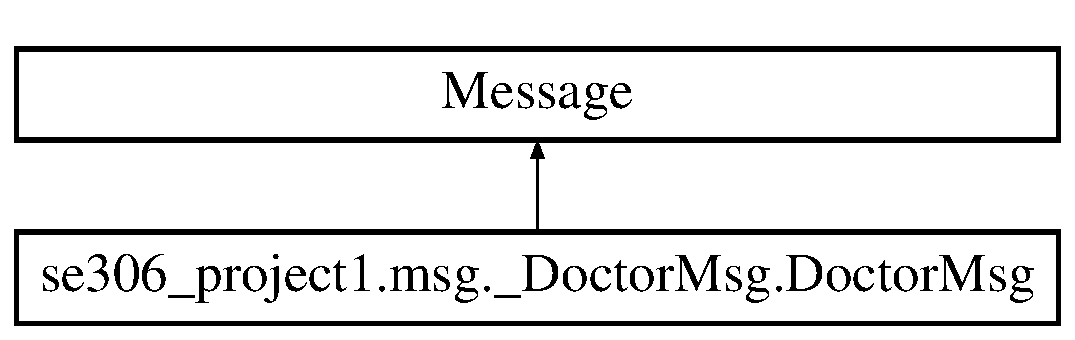
\includegraphics[height=2.000000cm]{classse306__project1_1_1msg_1_1__DoctorMsg_1_1DoctorMsg}
\end{center}
\end{figure}
\subsection*{Public Member Functions}
\begin{DoxyCompactItemize}
\item 
def \hyperlink{classse306__project1_1_1msg_1_1__DoctorMsg_1_1DoctorMsg_acdab3728232479c2431f3dad412d3289}{\-\_\-\-\_\-init\-\_\-\-\_\-}
\item 
def \hyperlink{classse306__project1_1_1msg_1_1__DoctorMsg_1_1DoctorMsg_a17a7a9c4016eecae4ec0da40bbd86e31}{serialize}
\item 
def \hyperlink{classse306__project1_1_1msg_1_1__DoctorMsg_1_1DoctorMsg_ae585ea7a7ad1bf035a68ad1d5eebd081}{deserialize}
\item 
def \hyperlink{classse306__project1_1_1msg_1_1__DoctorMsg_1_1DoctorMsg_a754dadda899fe2abb3b84b8f7ee62ef0}{serialize\-\_\-numpy}
\item 
def \hyperlink{classse306__project1_1_1msg_1_1__DoctorMsg_1_1DoctorMsg_afb7de726ee1e81daf506f49c726d4d6c}{deserialize\-\_\-numpy}
\end{DoxyCompactItemize}
\subsection*{Public Attributes}
\begin{DoxyCompactItemize}
\item 
\hypertarget{classse306__project1_1_1msg_1_1__DoctorMsg_1_1DoctorMsg_aa20dd11e923c7737e98f9ca4bb7f9e82}{{\bfseries Resident\-Healed}}\label{classse306__project1_1_1msg_1_1__DoctorMsg_1_1DoctorMsg_aa20dd11e923c7737e98f9ca4bb7f9e82}

\item 
\hypertarget{classse306__project1_1_1msg_1_1__DoctorMsg_1_1DoctorMsg_ac6bb215d503205f44b153bc8ba88a2c0}{{\bfseries hospitalise}}\label{classse306__project1_1_1msg_1_1__DoctorMsg_1_1DoctorMsg_ac6bb215d503205f44b153bc8ba88a2c0}

\end{DoxyCompactItemize}


\subsection{Constructor \& Destructor Documentation}
\hypertarget{classse306__project1_1_1msg_1_1__DoctorMsg_1_1DoctorMsg_acdab3728232479c2431f3dad412d3289}{\index{se306\-\_\-project1\-::msg\-::\-\_\-\-Doctor\-Msg\-::\-Doctor\-Msg@{se306\-\_\-project1\-::msg\-::\-\_\-\-Doctor\-Msg\-::\-Doctor\-Msg}!\-\_\-\-\_\-init\-\_\-\-\_\-@{\-\_\-\-\_\-init\-\_\-\-\_\-}}
\index{\-\_\-\-\_\-init\-\_\-\-\_\-@{\-\_\-\-\_\-init\-\_\-\-\_\-}!se306_project1::msg::_DoctorMsg::DoctorMsg@{se306\-\_\-project1\-::msg\-::\-\_\-\-Doctor\-Msg\-::\-Doctor\-Msg}}
\subsubsection[{\-\_\-\-\_\-init\-\_\-\-\_\-}]{\setlength{\rightskip}{0pt plus 5cm}def se306\-\_\-project1.\-msg.\-\_\-\-Doctor\-Msg.\-Doctor\-Msg.\-\_\-\-\_\-init\-\_\-\-\_\- (
\begin{DoxyParamCaption}
\item[{}]{self, }
\item[{}]{args, }
\item[{}]{kwds}
\end{DoxyParamCaption}
)}}\label{classse306__project1_1_1msg_1_1__DoctorMsg_1_1DoctorMsg_acdab3728232479c2431f3dad412d3289}
\begin{DoxyVerb}Constructor. Any message fields that are implicitly/explicitly
set to None will be assigned a default value. The recommend
use is keyword arguments as this is more robust to future message
changes.  You cannot mix in-order arguments and keyword arguments.

The available fields are:
   ResidentHealed,hospitalise

:param args: complete set of field values, in .msg order
:param kwds: use keyword arguments corresponding to message field names
to set specific fields.
\end{DoxyVerb}
 

\subsection{Member Function Documentation}
\hypertarget{classse306__project1_1_1msg_1_1__DoctorMsg_1_1DoctorMsg_ae585ea7a7ad1bf035a68ad1d5eebd081}{\index{se306\-\_\-project1\-::msg\-::\-\_\-\-Doctor\-Msg\-::\-Doctor\-Msg@{se306\-\_\-project1\-::msg\-::\-\_\-\-Doctor\-Msg\-::\-Doctor\-Msg}!deserialize@{deserialize}}
\index{deserialize@{deserialize}!se306_project1::msg::_DoctorMsg::DoctorMsg@{se306\-\_\-project1\-::msg\-::\-\_\-\-Doctor\-Msg\-::\-Doctor\-Msg}}
\subsubsection[{deserialize}]{\setlength{\rightskip}{0pt plus 5cm}def se306\-\_\-project1.\-msg.\-\_\-\-Doctor\-Msg.\-Doctor\-Msg.\-deserialize (
\begin{DoxyParamCaption}
\item[{}]{self, }
\item[{}]{str}
\end{DoxyParamCaption}
)}}\label{classse306__project1_1_1msg_1_1__DoctorMsg_1_1DoctorMsg_ae585ea7a7ad1bf035a68ad1d5eebd081}
\begin{DoxyVerb}unpack serialized message in str into this message instance
:param str: byte array of serialized message, ``str``
\end{DoxyVerb}
 \hypertarget{classse306__project1_1_1msg_1_1__DoctorMsg_1_1DoctorMsg_afb7de726ee1e81daf506f49c726d4d6c}{\index{se306\-\_\-project1\-::msg\-::\-\_\-\-Doctor\-Msg\-::\-Doctor\-Msg@{se306\-\_\-project1\-::msg\-::\-\_\-\-Doctor\-Msg\-::\-Doctor\-Msg}!deserialize\-\_\-numpy@{deserialize\-\_\-numpy}}
\index{deserialize\-\_\-numpy@{deserialize\-\_\-numpy}!se306_project1::msg::_DoctorMsg::DoctorMsg@{se306\-\_\-project1\-::msg\-::\-\_\-\-Doctor\-Msg\-::\-Doctor\-Msg}}
\subsubsection[{deserialize\-\_\-numpy}]{\setlength{\rightskip}{0pt plus 5cm}def se306\-\_\-project1.\-msg.\-\_\-\-Doctor\-Msg.\-Doctor\-Msg.\-deserialize\-\_\-numpy (
\begin{DoxyParamCaption}
\item[{}]{self, }
\item[{}]{str, }
\item[{}]{numpy}
\end{DoxyParamCaption}
)}}\label{classse306__project1_1_1msg_1_1__DoctorMsg_1_1DoctorMsg_afb7de726ee1e81daf506f49c726d4d6c}
\begin{DoxyVerb}unpack serialized message in str into this message instance using numpy for array types
:param str: byte array of serialized message, ``str``
:param numpy: numpy python module
\end{DoxyVerb}
 \hypertarget{classse306__project1_1_1msg_1_1__DoctorMsg_1_1DoctorMsg_a17a7a9c4016eecae4ec0da40bbd86e31}{\index{se306\-\_\-project1\-::msg\-::\-\_\-\-Doctor\-Msg\-::\-Doctor\-Msg@{se306\-\_\-project1\-::msg\-::\-\_\-\-Doctor\-Msg\-::\-Doctor\-Msg}!serialize@{serialize}}
\index{serialize@{serialize}!se306_project1::msg::_DoctorMsg::DoctorMsg@{se306\-\_\-project1\-::msg\-::\-\_\-\-Doctor\-Msg\-::\-Doctor\-Msg}}
\subsubsection[{serialize}]{\setlength{\rightskip}{0pt plus 5cm}def se306\-\_\-project1.\-msg.\-\_\-\-Doctor\-Msg.\-Doctor\-Msg.\-serialize (
\begin{DoxyParamCaption}
\item[{}]{self, }
\item[{}]{buff}
\end{DoxyParamCaption}
)}}\label{classse306__project1_1_1msg_1_1__DoctorMsg_1_1DoctorMsg_a17a7a9c4016eecae4ec0da40bbd86e31}
\begin{DoxyVerb}serialize message into buffer
:param buff: buffer, ``StringIO``
\end{DoxyVerb}
 \hypertarget{classse306__project1_1_1msg_1_1__DoctorMsg_1_1DoctorMsg_a754dadda899fe2abb3b84b8f7ee62ef0}{\index{se306\-\_\-project1\-::msg\-::\-\_\-\-Doctor\-Msg\-::\-Doctor\-Msg@{se306\-\_\-project1\-::msg\-::\-\_\-\-Doctor\-Msg\-::\-Doctor\-Msg}!serialize\-\_\-numpy@{serialize\-\_\-numpy}}
\index{serialize\-\_\-numpy@{serialize\-\_\-numpy}!se306_project1::msg::_DoctorMsg::DoctorMsg@{se306\-\_\-project1\-::msg\-::\-\_\-\-Doctor\-Msg\-::\-Doctor\-Msg}}
\subsubsection[{serialize\-\_\-numpy}]{\setlength{\rightskip}{0pt plus 5cm}def se306\-\_\-project1.\-msg.\-\_\-\-Doctor\-Msg.\-Doctor\-Msg.\-serialize\-\_\-numpy (
\begin{DoxyParamCaption}
\item[{}]{self, }
\item[{}]{buff, }
\item[{}]{numpy}
\end{DoxyParamCaption}
)}}\label{classse306__project1_1_1msg_1_1__DoctorMsg_1_1DoctorMsg_a754dadda899fe2abb3b84b8f7ee62ef0}
\begin{DoxyVerb}serialize message with numpy array types into buffer
:param buff: buffer, ``StringIO``
:param numpy: numpy python module
\end{DoxyVerb}
 

The documentation for this class was generated from the following file\-:\begin{DoxyCompactItemize}
\item 
se306\-\_\-project1/src/se306\-\_\-project1/msg/\-\_\-\-Doctor\-Msg.\-py\end{DoxyCompactItemize}

\hypertarget{structse306__project1_1_1DoctorMsg__}{\section{se306\-\_\-project1\-:\-:Doctor\-Msg\-\_\-$<$ Container\-Allocator $>$ Struct Template Reference}
\label{structse306__project1_1_1DoctorMsg__}\index{se306\-\_\-project1\-::\-Doctor\-Msg\-\_\-$<$ Container\-Allocator $>$@{se306\-\_\-project1\-::\-Doctor\-Msg\-\_\-$<$ Container\-Allocator $>$}}
}
\subsection*{Public Types}
\begin{DoxyCompactItemize}
\item 
\hypertarget{structse306__project1_1_1DoctorMsg___a00781357575cf134c091219ee53d0a94}{typedef \hyperlink{structse306__project1_1_1DoctorMsg__}{Doctor\-Msg\-\_\-}\\*
$<$ Container\-Allocator $>$ {\bfseries Type}}\label{structse306__project1_1_1DoctorMsg___a00781357575cf134c091219ee53d0a94}

\item 
\hypertarget{structse306__project1_1_1DoctorMsg___ab3b22428daa95b3a0a085e3b64af8d39}{typedef uint8\-\_\-t {\bfseries \-\_\-\-Resident\-Healed\-\_\-type}}\label{structse306__project1_1_1DoctorMsg___ab3b22428daa95b3a0a085e3b64af8d39}

\item 
\hypertarget{structse306__project1_1_1DoctorMsg___a87354ca763be48d0e501a23f1870268c}{typedef uint8\-\_\-t {\bfseries \-\_\-hospitalise\-\_\-type}}\label{structse306__project1_1_1DoctorMsg___a87354ca763be48d0e501a23f1870268c}

\item 
\hypertarget{structse306__project1_1_1DoctorMsg___a8a5d1bbf5000de3e2d58770fc41be09d}{typedef boost\-::shared\-\_\-ptr\\*
$<$ \-::\hyperlink{structse306__project1_1_1DoctorMsg__}{se306\-\_\-project1\-::\-Doctor\-Msg\-\_\-}\\*
$<$ Container\-Allocator $>$ $>$ {\bfseries Ptr}}\label{structse306__project1_1_1DoctorMsg___a8a5d1bbf5000de3e2d58770fc41be09d}

\item 
\hypertarget{structse306__project1_1_1DoctorMsg___af7d7e47c79b0848918536b70a58a4a8e}{typedef boost\-::shared\-\_\-ptr\\*
$<$ \-::\hyperlink{structse306__project1_1_1DoctorMsg__}{se306\-\_\-project1\-::\-Doctor\-Msg\-\_\-}\\*
$<$ Container\-Allocator $>$ const  $>$ {\bfseries Const\-Ptr}}\label{structse306__project1_1_1DoctorMsg___af7d7e47c79b0848918536b70a58a4a8e}

\end{DoxyCompactItemize}
\subsection*{Public Member Functions}
\begin{DoxyCompactItemize}
\item 
\hypertarget{structse306__project1_1_1DoctorMsg___a011e25faaa89c7cc8a34e8ef14c9e486}{{\bfseries Doctor\-Msg\-\_\-} (const Container\-Allocator \&\-\_\-alloc)}\label{structse306__project1_1_1DoctorMsg___a011e25faaa89c7cc8a34e8ef14c9e486}

\end{DoxyCompactItemize}
\subsection*{Public Attributes}
\begin{DoxyCompactItemize}
\item 
\hypertarget{structse306__project1_1_1DoctorMsg___a920e464dbcb861b061ef834a386d5b9f}{uint8\-\_\-t {\bfseries Resident\-Healed}}\label{structse306__project1_1_1DoctorMsg___a920e464dbcb861b061ef834a386d5b9f}

\item 
\hypertarget{structse306__project1_1_1DoctorMsg___a1c3941a076ae6d80ce7f8e514c5021a9}{uint8\-\_\-t {\bfseries hospitalise}}\label{structse306__project1_1_1DoctorMsg___a1c3941a076ae6d80ce7f8e514c5021a9}

\end{DoxyCompactItemize}


The documentation for this struct was generated from the following file\-:\begin{DoxyCompactItemize}
\item 
se306\-\_\-project1/msg\-\_\-gen/cpp/include/se306\-\_\-project1/Doctor\-Msg.\-h\end{DoxyCompactItemize}

\hypertarget{classDoor}{\section{Door Class Reference}
\label{classDoor}\index{Door@{Door}}
}


Class for the \hyperlink{classDoor}{Door} nodes.  




{\ttfamily \#include $<$Door.\-h$>$}

\subsection*{Public Member Functions}
\begin{DoxyCompactItemize}
\item 
\hypertarget{classDoor_a6b8d9bba2d7cbaa3262887a209c3ffca}{int \hyperlink{classDoor_a6b8d9bba2d7cbaa3262887a209c3ffca}{run} (int argc, char $\ast$argv\mbox{[}$\,$\mbox{]})}\label{classDoor_a6b8d9bba2d7cbaa3262887a209c3ffca}

\begin{DoxyCompactList}\small\item\em Main function for the \hyperlink{classDoor}{Door} process. Controls node setup and periodic events. \end{DoxyCompactList}\end{DoxyCompactItemize}
\subsection*{Protected Member Functions}
\begin{DoxyCompactItemize}
\item 
void \hyperlink{classDoor_ae2c0e2da31af301f0761fad9618df595}{Stage\-Odom\-\_\-callback} (nav\-\_\-msgs\-::\-Odometry msg)
\begin{DoxyCompactList}\small\item\em Updates the door's x position, y position, and angle to reflect its current pose. \end{DoxyCompactList}\item 
void \hyperlink{classDoor_afe7ef9a01779f3cc6285ed0350175261}{delegate} (\hyperlink{structse306__project1_1_1ResidentMsg__}{se306\-\_\-project1\-::\-Resident\-Msg} msg)
\begin{DoxyCompactList}\small\item\em Callback function that unpacks and processes resident status messages. \hyperlink{classDoor}{Door} should subscribe to the Resident\-Msg topic in order for this callback to be called. Resident\-Msg is published by the \hyperlink{classResident}{Resident}. \end{DoxyCompactList}\item 
\hypertarget{classDoor_a141b8ac2ab99e1d7a218cdfb52004937}{void \hyperlink{classDoor_a141b8ac2ab99e1d7a218cdfb52004937}{open} ()}\label{classDoor_a141b8ac2ab99e1d7a218cdfb52004937}

\begin{DoxyCompactList}\small\item\em opens the \hyperlink{classDoor}{Door} \end{DoxyCompactList}\item 
\hypertarget{classDoor_a1610991c042246a8d66421201667e361}{void \hyperlink{classDoor_a1610991c042246a8d66421201667e361}{close} (int wait\-Time)}\label{classDoor_a1610991c042246a8d66421201667e361}

\begin{DoxyCompactList}\small\item\em closes the \hyperlink{classDoor}{Door} after being opened for 20 seconds \end{DoxyCompactList}\end{DoxyCompactItemize}


\subsection{Detailed Description}
Class for the \hyperlink{classDoor}{Door} nodes. 

\subsection{Member Function Documentation}
\hypertarget{classDoor_afe7ef9a01779f3cc6285ed0350175261}{\index{Door@{Door}!delegate@{delegate}}
\index{delegate@{delegate}!Door@{Door}}
\subsubsection[{delegate}]{\setlength{\rightskip}{0pt plus 5cm}void Door\-::delegate (
\begin{DoxyParamCaption}
\item[{{\bf se306\-\_\-project1\-::\-Resident\-Msg}}]{msg}
\end{DoxyParamCaption}
)\hspace{0.3cm}{\ttfamily [protected]}}}\label{classDoor_afe7ef9a01779f3cc6285ed0350175261}


Callback function that unpacks and processes resident status messages. \hyperlink{classDoor}{Door} should subscribe to the Resident\-Msg topic in order for this callback to be called. Resident\-Msg is published by the \hyperlink{classResident}{Resident}. 


\begin{DoxyParams}{Parameters}
{\em msg} & A custom Resident\-Msg message that contains information about the resident's current status. \\
\hline
\end{DoxyParams}
\hypertarget{classDoor_ae2c0e2da31af301f0761fad9618df595}{\index{Door@{Door}!Stage\-Odom\-\_\-callback@{Stage\-Odom\-\_\-callback}}
\index{Stage\-Odom\-\_\-callback@{Stage\-Odom\-\_\-callback}!Door@{Door}}
\subsubsection[{Stage\-Odom\-\_\-callback}]{\setlength{\rightskip}{0pt plus 5cm}void Door\-::\-Stage\-Odom\-\_\-callback (
\begin{DoxyParamCaption}
\item[{nav\-\_\-msgs\-::\-Odometry}]{msg}
\end{DoxyParamCaption}
)\hspace{0.3cm}{\ttfamily [protected]}}}\label{classDoor_ae2c0e2da31af301f0761fad9618df595}


Updates the door's x position, y position, and angle to reflect its current pose. 


\begin{DoxyParams}{Parameters}
{\em msg} & Odometry message from odom topic \\
\hline
\end{DoxyParams}


The documentation for this class was generated from the following files\-:\begin{DoxyCompactItemize}
\item 
se306\-\_\-project1/src/Door.\-h\item 
se306\-\_\-project1/src/Door.\-cpp\end{DoxyCompactItemize}

\hypertarget{classFriend}{\section{Friend Class Reference}
\label{classFriend}\index{Friend@{Friend}}
}


Class for \hyperlink{classFriend}{Friend} nodes.  




{\ttfamily \#include $<$Friend.\-h$>$}

Inheritance diagram for Friend\-:\begin{figure}[H]
\begin{center}
\leavevmode
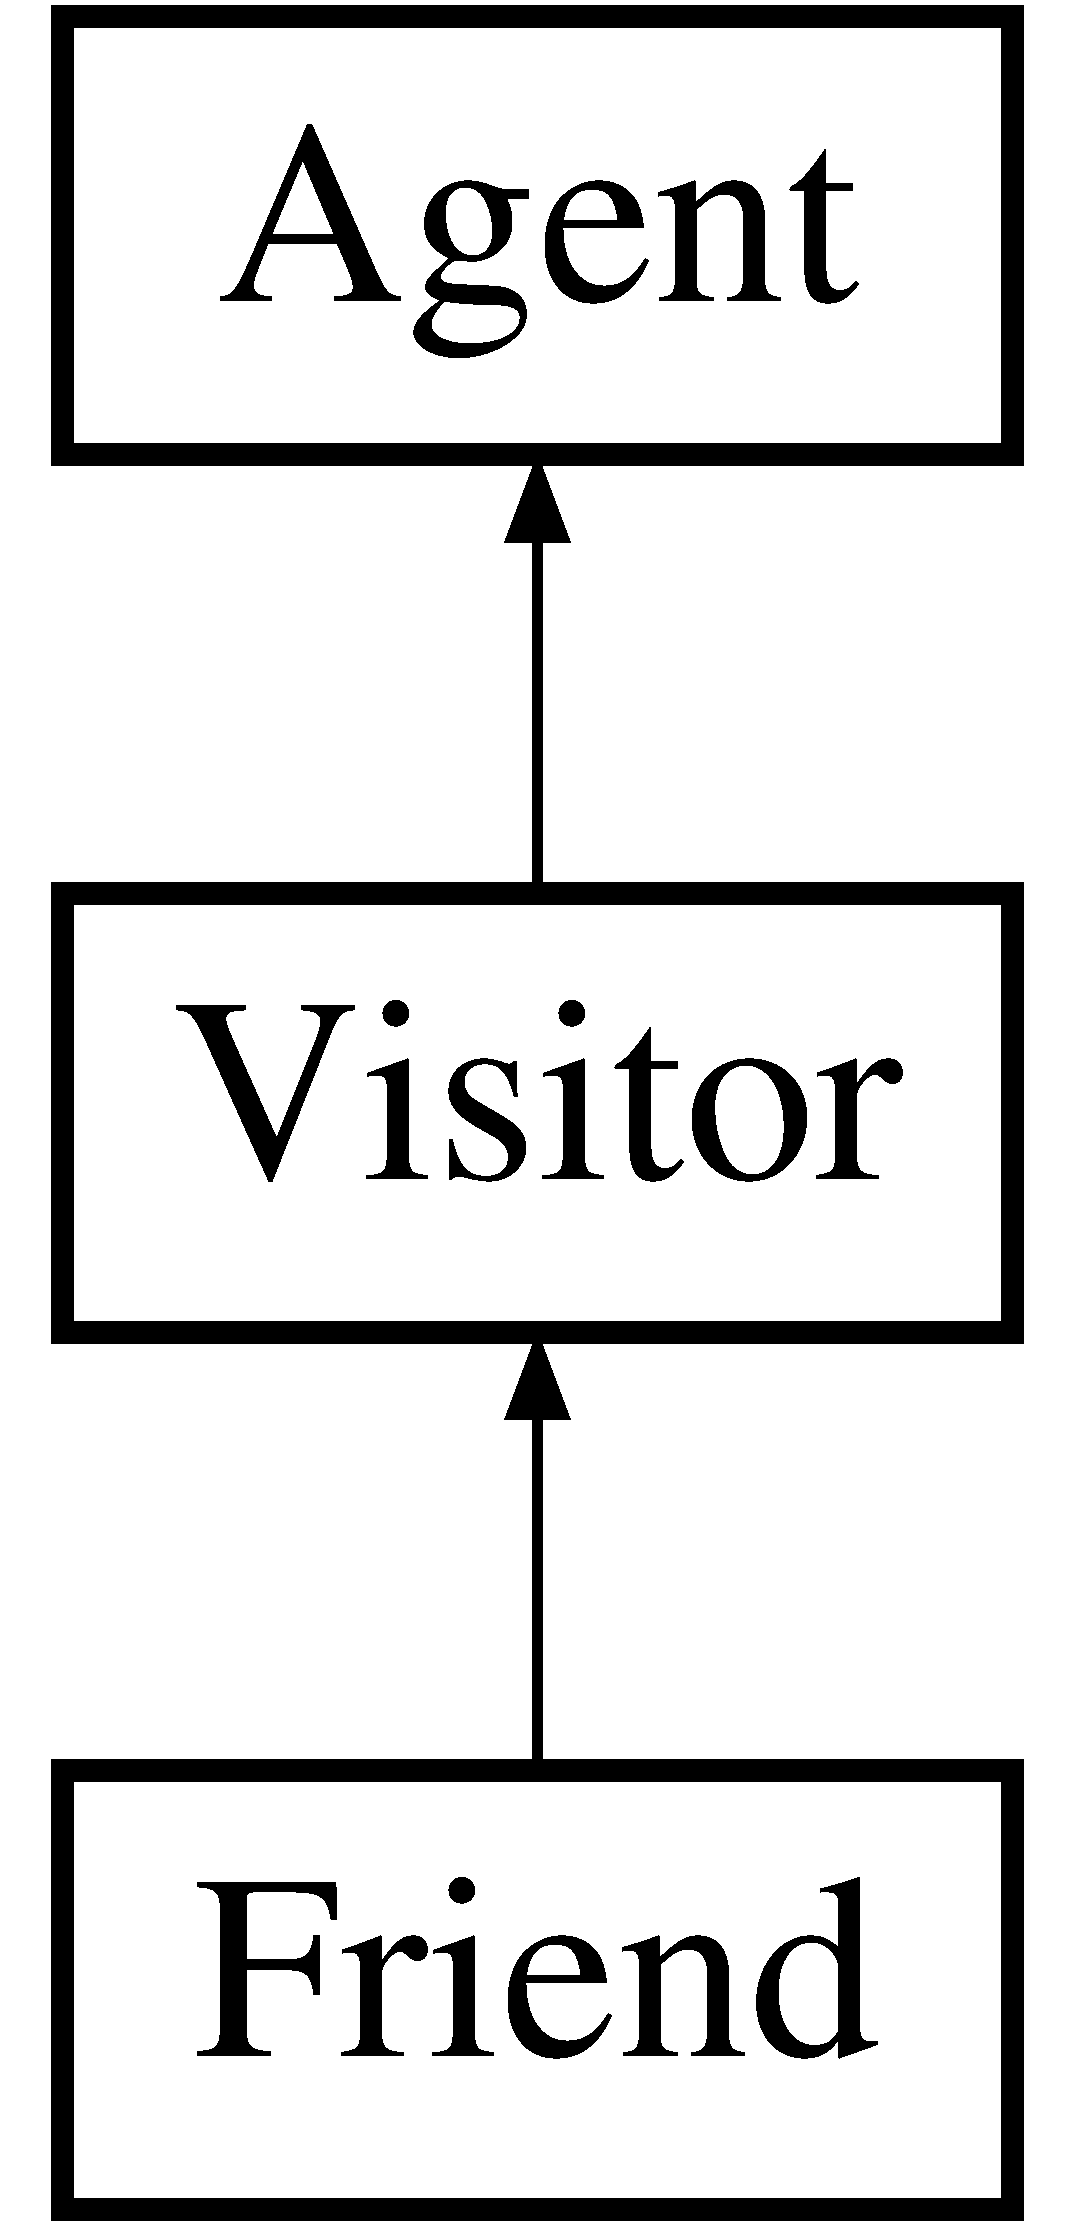
\includegraphics[height=3.000000cm]{classFriend}
\end{center}
\end{figure}
\subsection*{Public Member Functions}
\begin{DoxyCompactItemize}
\item 
void \hyperlink{classFriend_ab336b2a40bc6b9787bd0e9283f29f468}{Stage\-Odom\-\_\-callback} (nav\-\_\-msgs\-::\-Odometry msg)
\begin{DoxyCompactList}\small\item\em Updates the \hyperlink{classFriend}{Friend}'s x position, y position, and angle to reflect its current pose. \end{DoxyCompactList}\item 
void \hyperlink{classFriend_a1334996a432a7d435d40169bad684dc4}{Stage\-Laser\-\_\-callback} (sensor\-\_\-msgs\-::\-Laser\-Scan msg)
\begin{DoxyCompactList}\small\item\em Callback function to process laser scan messsages. You can access the range data from msg.\-ranges\mbox{[}i\mbox{]}. i = sample number. \end{DoxyCompactList}\item 
\hypertarget{classFriend_a0a4bf249b808ade72706f8f0a639ccde}{int \hyperlink{classFriend_a0a4bf249b808ade72706f8f0a639ccde}{run} (int argc, char $\ast$argv\mbox{[}$\,$\mbox{]})}\label{classFriend_a0a4bf249b808ade72706f8f0a639ccde}

\begin{DoxyCompactList}\small\item\em Main function for the \hyperlink{classFriend}{Friend} process. Controls node setup and periodic events. \end{DoxyCompactList}\end{DoxyCompactItemize}
\subsection*{Additional Inherited Members}


\subsection{Detailed Description}
Class for \hyperlink{classFriend}{Friend} nodes. 

\subsection{Member Function Documentation}
\hypertarget{classFriend_a1334996a432a7d435d40169bad684dc4}{\index{Friend@{Friend}!Stage\-Laser\-\_\-callback@{Stage\-Laser\-\_\-callback}}
\index{Stage\-Laser\-\_\-callback@{Stage\-Laser\-\_\-callback}!Friend@{Friend}}
\subsubsection[{Stage\-Laser\-\_\-callback}]{\setlength{\rightskip}{0pt plus 5cm}void Friend\-::\-Stage\-Laser\-\_\-callback (
\begin{DoxyParamCaption}
\item[{sensor\-\_\-msgs\-::\-Laser\-Scan}]{msg}
\end{DoxyParamCaption}
)\hspace{0.3cm}{\ttfamily [virtual]}}}\label{classFriend_a1334996a432a7d435d40169bad684dc4}


Callback function to process laser scan messsages. You can access the range data from msg.\-ranges\mbox{[}i\mbox{]}. i = sample number. 

\begin{DoxyNote}{Note}
Currently blank as it is not in use. Navigation operates through a checkpoint system. 
\end{DoxyNote}

\begin{DoxyParams}{Parameters}
{\em msg} & Single scan from a planar laser range finder \\
\hline
\end{DoxyParams}


Implements \hyperlink{classAgent_adfe1de8bbeaa7e4a5f7f2ff3e45593e8}{Agent}.

\hypertarget{classFriend_ab336b2a40bc6b9787bd0e9283f29f468}{\index{Friend@{Friend}!Stage\-Odom\-\_\-callback@{Stage\-Odom\-\_\-callback}}
\index{Stage\-Odom\-\_\-callback@{Stage\-Odom\-\_\-callback}!Friend@{Friend}}
\subsubsection[{Stage\-Odom\-\_\-callback}]{\setlength{\rightskip}{0pt plus 5cm}void Friend\-::\-Stage\-Odom\-\_\-callback (
\begin{DoxyParamCaption}
\item[{nav\-\_\-msgs\-::\-Odometry}]{msg}
\end{DoxyParamCaption}
)\hspace{0.3cm}{\ttfamily [virtual]}}}\label{classFriend_ab336b2a40bc6b9787bd0e9283f29f468}


Updates the \hyperlink{classFriend}{Friend}'s x position, y position, and angle to reflect its current pose. 

\begin{DoxyNote}{Note}
Rounding is used to calculate the current angle. This approximation is accounted for by using threshholds when processing angles. 
\end{DoxyNote}

\begin{DoxyParams}{Parameters}
{\em msg} & Odometry message from odom topic \\
\hline
\end{DoxyParams}


Implements \hyperlink{classAgent_a4b1182b9ee5dccaa871d71beef94a7d2}{Agent}.



The documentation for this class was generated from the following files\-:\begin{DoxyCompactItemize}
\item 
se306\-\_\-project1/src/Friend.\-h\item 
se306\-\_\-project1/src/Friend.\-cpp\end{DoxyCompactItemize}

\hypertarget{classFriend1}{\section{Friend1 Class Reference}
\label{classFriend1}\index{Friend1@{Friend1}}
}


Class for \hyperlink{classFriend}{Friend} nodes.  




{\ttfamily \#include $<$Friend1.\-h$>$}

Inheritance diagram for Friend1\-:\begin{figure}[H]
\begin{center}
\leavevmode
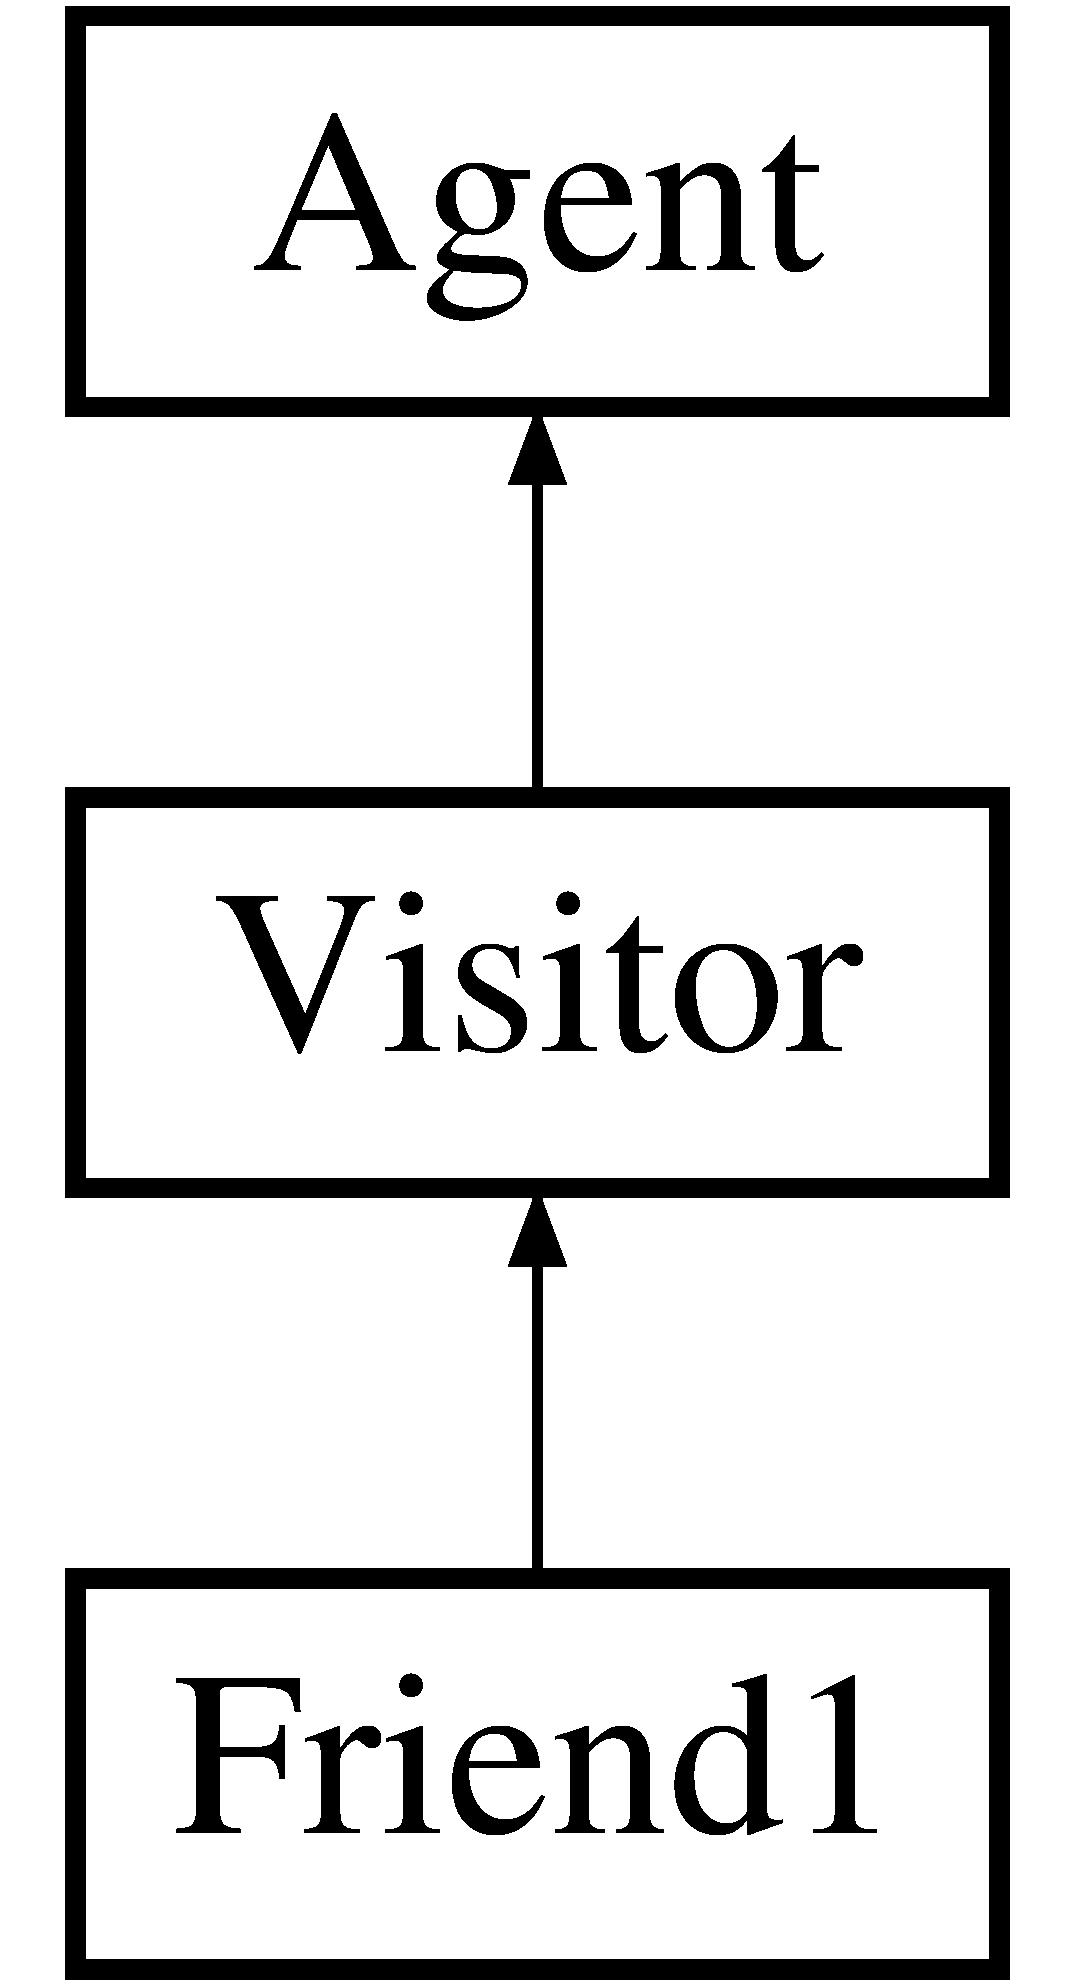
\includegraphics[height=3.000000cm]{classFriend1}
\end{center}
\end{figure}
\subsection*{Public Member Functions}
\begin{DoxyCompactItemize}
\item 
\hypertarget{classFriend1_af76fdf88c44de0410ad51c9290e88a4e}{int \hyperlink{classFriend1_af76fdf88c44de0410ad51c9290e88a4e}{run} (int argc, char $\ast$argv\mbox{[}$\,$\mbox{]})}\label{classFriend1_af76fdf88c44de0410ad51c9290e88a4e}

\begin{DoxyCompactList}\small\item\em Main function for the \hyperlink{classFriend}{Friend} process. Controls node setup and periodic events. \end{DoxyCompactList}\item 
\hypertarget{classFriend1_a18a2d1c5a80fd0b2c13bc4001fae540b}{void {\bfseries friends\-Done\-Callback} (const ros\-::\-Timer\-Event \&)}\label{classFriend1_a18a2d1c5a80fd0b2c13bc4001fae540b}

\end{DoxyCompactItemize}
\subsection*{Protected Member Functions}
\begin{DoxyCompactItemize}
\item 
void \hyperlink{classFriend1_a6b17166cc8b1a509c15e13ddfc11f773}{delegate} (\hyperlink{structse306__project1_1_1ResidentMsg__}{se306\-\_\-project1\-::\-Resident\-Msg} msg)
\begin{DoxyCompactList}\small\item\em Callback function that unpacks and processes resident status messages. \hyperlink{classFriend}{Friend} should subscribe to the Resident\-Msg topic in order for this callback to be called. Resident\-Msg is published by the \hyperlink{classResident}{Resident}. \end{DoxyCompactList}\item 
\hypertarget{classFriend1_a6e2bc30169674b4a5c038c8f2fd2c1a1}{void {\bfseries do\-Timed\-Visit} (const ros\-::\-Timer\-Event \&)}\label{classFriend1_a6e2bc30169674b4a5c038c8f2fd2c1a1}

\end{DoxyCompactItemize}
\subsection*{Additional Inherited Members}


\subsection{Detailed Description}
Class for \hyperlink{classFriend}{Friend} nodes. 

\subsection{Member Function Documentation}
\hypertarget{classFriend1_a6b17166cc8b1a509c15e13ddfc11f773}{\index{Friend1@{Friend1}!delegate@{delegate}}
\index{delegate@{delegate}!Friend1@{Friend1}}
\subsubsection[{delegate}]{\setlength{\rightskip}{0pt plus 5cm}void Friend1\-::delegate (
\begin{DoxyParamCaption}
\item[{{\bf se306\-\_\-project1\-::\-Resident\-Msg}}]{msg}
\end{DoxyParamCaption}
)\hspace{0.3cm}{\ttfamily [protected]}}}\label{classFriend1_a6b17166cc8b1a509c15e13ddfc11f773}


Callback function that unpacks and processes resident status messages. \hyperlink{classFriend}{Friend} should subscribe to the Resident\-Msg topic in order for this callback to be called. Resident\-Msg is published by the \hyperlink{classResident}{Resident}. 


\begin{DoxyParams}{Parameters}
{\em msg} & A custom Resident\-Msg message that contains information about the resident's current status. \\
\hline
\end{DoxyParams}


The documentation for this class was generated from the following files\-:\begin{DoxyCompactItemize}
\item 
se306\-\_\-project1/src/Friend1.\-h\item 
se306\-\_\-project1/src/Friend1.\-cpp\end{DoxyCompactItemize}

\hypertarget{classFriend2}{\section{Friend2 Class Reference}
\label{classFriend2}\index{Friend2@{Friend2}}
}


Class for \hyperlink{classFriend}{Friend} nodes.  




{\ttfamily \#include $<$Friend2.\-h$>$}

Inheritance diagram for Friend2\-:\begin{figure}[H]
\begin{center}
\leavevmode
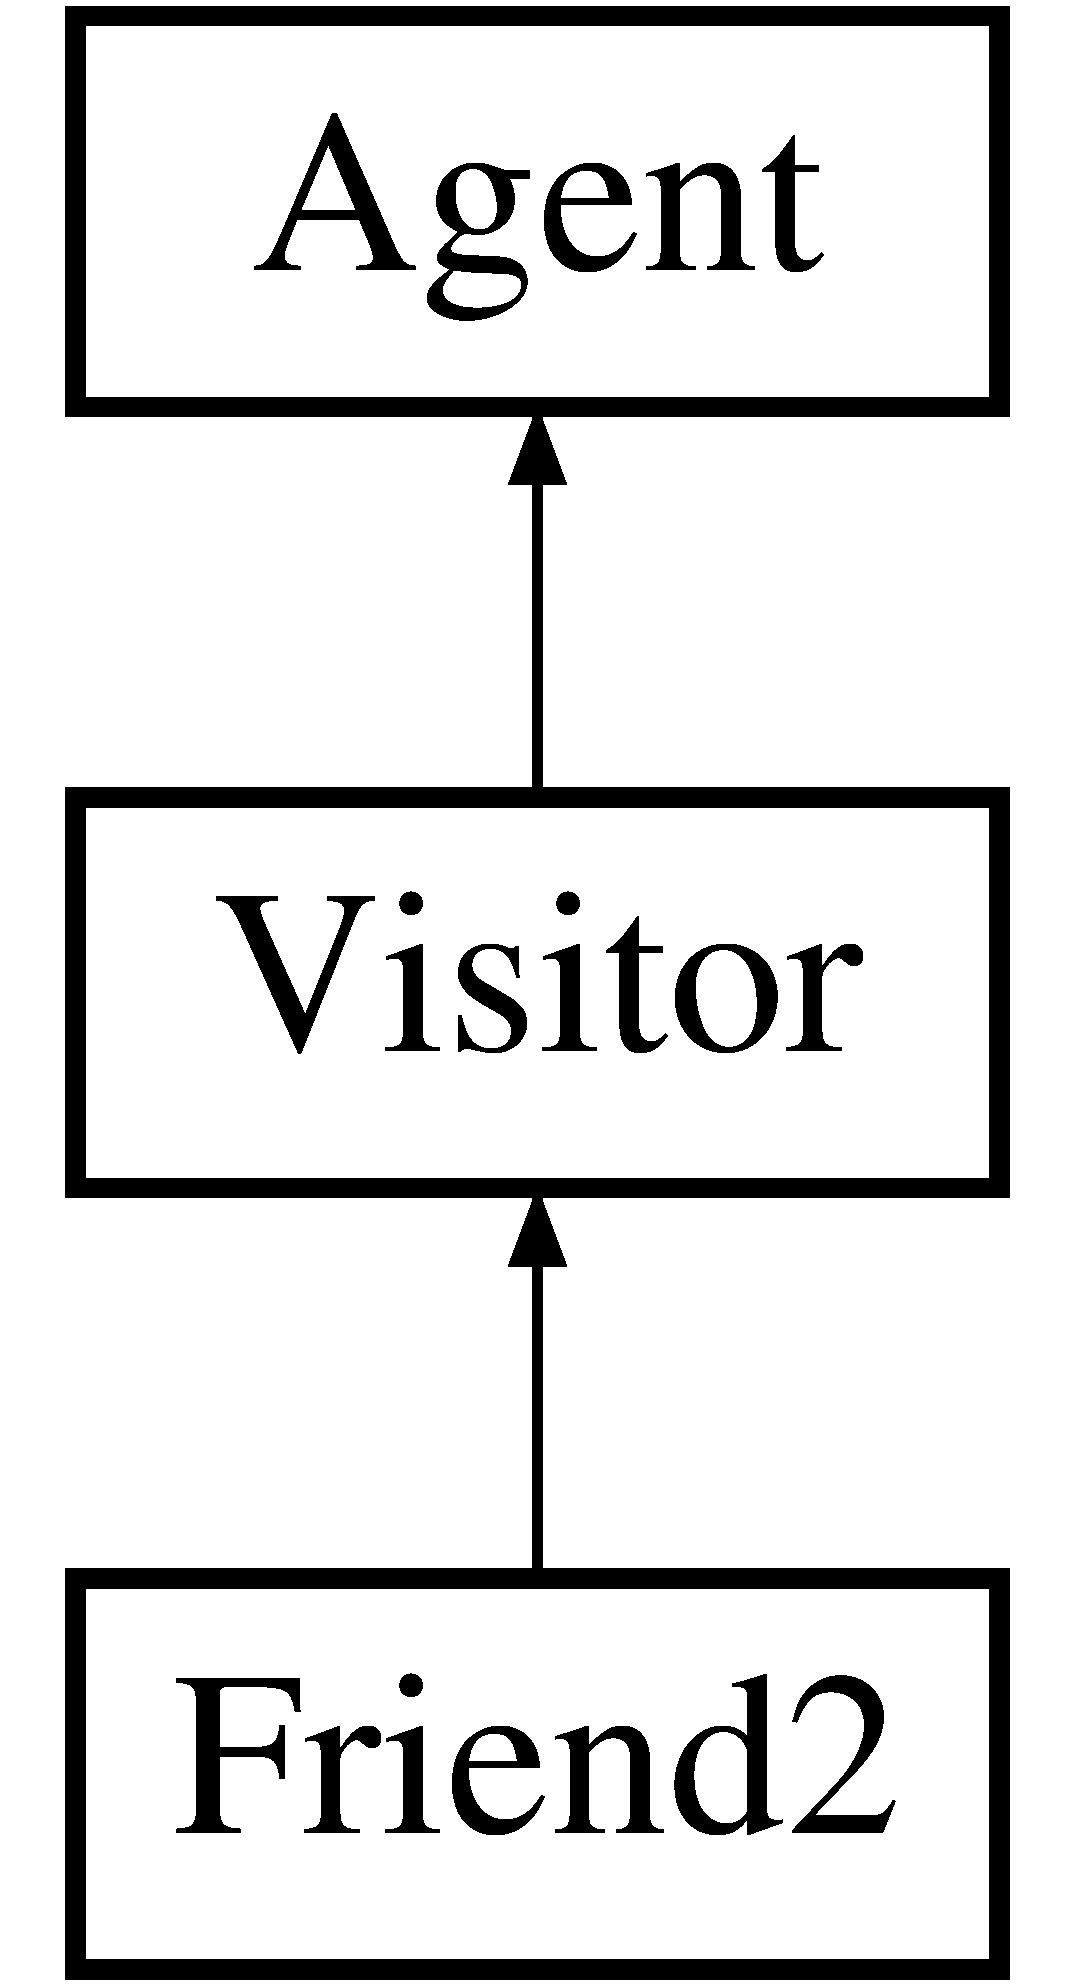
\includegraphics[height=3.000000cm]{classFriend2}
\end{center}
\end{figure}
\subsection*{Public Member Functions}
\begin{DoxyCompactItemize}
\item 
\hypertarget{classFriend2_ad03c02e64256ea572ca3dfbf4bba0d0e}{int \hyperlink{classFriend2_ad03c02e64256ea572ca3dfbf4bba0d0e}{run} (int argc, char $\ast$argv\mbox{[}$\,$\mbox{]})}\label{classFriend2_ad03c02e64256ea572ca3dfbf4bba0d0e}

\begin{DoxyCompactList}\small\item\em Main function for the \hyperlink{classFriend}{Friend} process. Controls node setup and periodic events. \end{DoxyCompactList}\item 
\hypertarget{classFriend2_a4d8cfc5c44393e2353349197894d8393}{void \hyperlink{classFriend2_a4d8cfc5c44393e2353349197894d8393}{friends\-Done\-Callback} (const ros\-::\-Timer\-Event \&)}\label{classFriend2_a4d8cfc5c44393e2353349197894d8393}

\begin{DoxyCompactList}\small\item\em Returns the friend to its start point once its interaction with the resident is done. \end{DoxyCompactList}\end{DoxyCompactItemize}
\subsection*{Protected Member Functions}
\begin{DoxyCompactItemize}
\item 
void \hyperlink{classFriend2_a9739a9f4fe4e8768cfbf0849efc2d9c2}{delegate} (\hyperlink{structse306__project1_1_1ResidentMsg__}{se306\-\_\-project1\-::\-Resident\-Msg} msg)
\begin{DoxyCompactList}\small\item\em Callback function that unpacks and processes resident status messages. \hyperlink{classFriend}{Friend} should subscribe to the Resident\-Msg topic in order for this callback to be called. Resident\-Msg is published by the \hyperlink{classResident}{Resident}. \end{DoxyCompactList}\item 
\hypertarget{classFriend2_a6271e3b801a54915dbcc87cca56ba168}{void {\bfseries do\-Timed\-Visit} (const ros\-::\-Timer\-Event \&)}\label{classFriend2_a6271e3b801a54915dbcc87cca56ba168}

\end{DoxyCompactItemize}
\subsection*{Additional Inherited Members}


\subsection{Detailed Description}
Class for \hyperlink{classFriend}{Friend} nodes. 

\subsection{Member Function Documentation}
\hypertarget{classFriend2_a9739a9f4fe4e8768cfbf0849efc2d9c2}{\index{Friend2@{Friend2}!delegate@{delegate}}
\index{delegate@{delegate}!Friend2@{Friend2}}
\subsubsection[{delegate}]{\setlength{\rightskip}{0pt plus 5cm}void Friend2\-::delegate (
\begin{DoxyParamCaption}
\item[{{\bf se306\-\_\-project1\-::\-Resident\-Msg}}]{msg}
\end{DoxyParamCaption}
)\hspace{0.3cm}{\ttfamily [protected]}}}\label{classFriend2_a9739a9f4fe4e8768cfbf0849efc2d9c2}


Callback function that unpacks and processes resident status messages. \hyperlink{classFriend}{Friend} should subscribe to the Resident\-Msg topic in order for this callback to be called. Resident\-Msg is published by the \hyperlink{classResident}{Resident}. 


\begin{DoxyParams}{Parameters}
{\em msg} & A custom Resident\-Msg message that contains information about the resident's current status. \\
\hline
\end{DoxyParams}


The documentation for this class was generated from the following files\-:\begin{DoxyCompactItemize}
\item 
se306\-\_\-project1/src/Friend2.\-h\item 
se306\-\_\-project1/src/Friend2.\-cpp\end{DoxyCompactItemize}

\hypertarget{structros_1_1message__traits_1_1IsFixedSize_3_01_1_1se306__project1_1_1AssistantMsg___3_01ContainerAllocator_01_4_01_4}{\section{ros\-:\-:message\-\_\-traits\-:\-:Is\-Fixed\-Size$<$ \-:\-:se306\-\_\-project1\-:\-:Assistant\-Msg\-\_\-$<$ Container\-Allocator $>$ $>$ Struct Template Reference}
\label{structros_1_1message__traits_1_1IsFixedSize_3_01_1_1se306__project1_1_1AssistantMsg___3_01ContainerAllocator_01_4_01_4}\index{ros\-::message\-\_\-traits\-::\-Is\-Fixed\-Size$<$ \-::se306\-\_\-project1\-::\-Assistant\-Msg\-\_\-$<$ Container\-Allocator $>$ $>$@{ros\-::message\-\_\-traits\-::\-Is\-Fixed\-Size$<$ \-::se306\-\_\-project1\-::\-Assistant\-Msg\-\_\-$<$ Container\-Allocator $>$ $>$}}
}
Inheritance diagram for ros\-:\-:message\-\_\-traits\-:\-:Is\-Fixed\-Size$<$ \-:\-:se306\-\_\-project1\-:\-:Assistant\-Msg\-\_\-$<$ Container\-Allocator $>$ $>$\-:\begin{figure}[H]
\begin{center}
\leavevmode
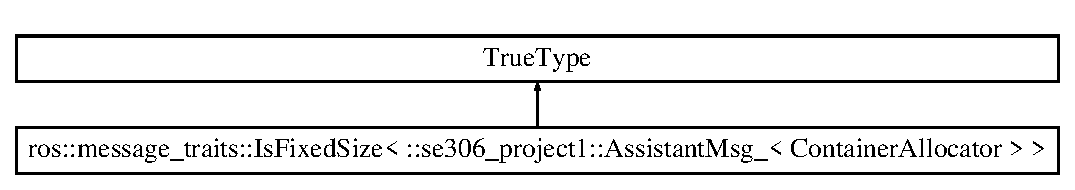
\includegraphics[height=2.000000cm]{structros_1_1message__traits_1_1IsFixedSize_3_01_1_1se306__project1_1_1AssistantMsg___3_01ContainerAllocator_01_4_01_4}
\end{center}
\end{figure}


The documentation for this struct was generated from the following file\-:\begin{DoxyCompactItemize}
\item 
se306\-\_\-project1/msg\-\_\-gen/cpp/include/se306\-\_\-project1/Assistant\-Msg.\-h\end{DoxyCompactItemize}

\hypertarget{structros_1_1message__traits_1_1IsFixedSize_3_01_1_1se306__project1_1_1DoctorMsg___3_01ContainerAllocator_01_4_01_4}{\section{ros\-:\-:message\-\_\-traits\-:\-:Is\-Fixed\-Size$<$ \-:\-:se306\-\_\-project1\-:\-:Doctor\-Msg\-\_\-$<$ Container\-Allocator $>$ $>$ Struct Template Reference}
\label{structros_1_1message__traits_1_1IsFixedSize_3_01_1_1se306__project1_1_1DoctorMsg___3_01ContainerAllocator_01_4_01_4}\index{ros\-::message\-\_\-traits\-::\-Is\-Fixed\-Size$<$ \-::se306\-\_\-project1\-::\-Doctor\-Msg\-\_\-$<$ Container\-Allocator $>$ $>$@{ros\-::message\-\_\-traits\-::\-Is\-Fixed\-Size$<$ \-::se306\-\_\-project1\-::\-Doctor\-Msg\-\_\-$<$ Container\-Allocator $>$ $>$}}
}
Inheritance diagram for ros\-:\-:message\-\_\-traits\-:\-:Is\-Fixed\-Size$<$ \-:\-:se306\-\_\-project1\-:\-:Doctor\-Msg\-\_\-$<$ Container\-Allocator $>$ $>$\-:\begin{figure}[H]
\begin{center}
\leavevmode
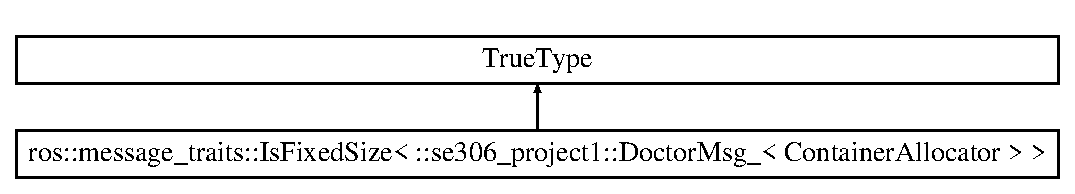
\includegraphics[height=2.000000cm]{structros_1_1message__traits_1_1IsFixedSize_3_01_1_1se306__project1_1_1DoctorMsg___3_01ContainerAllocator_01_4_01_4}
\end{center}
\end{figure}


The documentation for this struct was generated from the following file\-:\begin{DoxyCompactItemize}
\item 
se306\-\_\-project1/msg\-\_\-gen/cpp/include/se306\-\_\-project1/Doctor\-Msg.\-h\end{DoxyCompactItemize}

\hypertarget{structros_1_1message__traits_1_1IsMessage_3_01_1_1se306__project1_1_1AssistantMsg___3_01ContainerAllocator_01_4_01_4}{\section{ros\-:\-:message\-\_\-traits\-:\-:Is\-Message$<$ \-:\-:se306\-\_\-project1\-:\-:Assistant\-Msg\-\_\-$<$ Container\-Allocator $>$ $>$ Struct Template Reference}
\label{structros_1_1message__traits_1_1IsMessage_3_01_1_1se306__project1_1_1AssistantMsg___3_01ContainerAllocator_01_4_01_4}\index{ros\-::message\-\_\-traits\-::\-Is\-Message$<$ \-::se306\-\_\-project1\-::\-Assistant\-Msg\-\_\-$<$ Container\-Allocator $>$ $>$@{ros\-::message\-\_\-traits\-::\-Is\-Message$<$ \-::se306\-\_\-project1\-::\-Assistant\-Msg\-\_\-$<$ Container\-Allocator $>$ $>$}}
}
Inheritance diagram for ros\-:\-:message\-\_\-traits\-:\-:Is\-Message$<$ \-:\-:se306\-\_\-project1\-:\-:Assistant\-Msg\-\_\-$<$ Container\-Allocator $>$ $>$\-:\begin{figure}[H]
\begin{center}
\leavevmode
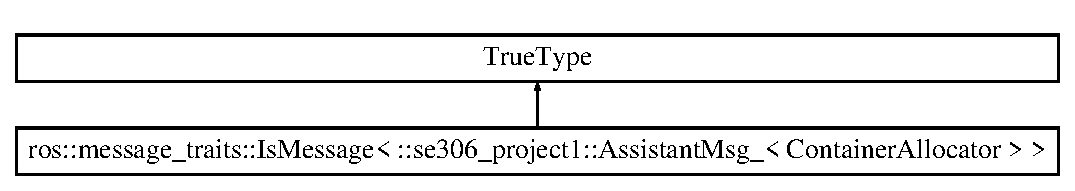
\includegraphics[height=2.000000cm]{structros_1_1message__traits_1_1IsMessage_3_01_1_1se306__project1_1_1AssistantMsg___3_01ContainerAllocator_01_4_01_4}
\end{center}
\end{figure}


The documentation for this struct was generated from the following file\-:\begin{DoxyCompactItemize}
\item 
se306\-\_\-project1/msg\-\_\-gen/cpp/include/se306\-\_\-project1/Assistant\-Msg.\-h\end{DoxyCompactItemize}

\hypertarget{structros_1_1message__traits_1_1IsMessage_3_01_1_1se306__project1_1_1AssistantMsg___3_01ContainerAllocator_01_4const_01_01_4}{\section{ros\-:\-:message\-\_\-traits\-:\-:Is\-Message$<$ \-:\-:se306\-\_\-project1\-:\-:Assistant\-Msg\-\_\-$<$ Container\-Allocator $>$const $>$ Struct Template Reference}
\label{structros_1_1message__traits_1_1IsMessage_3_01_1_1se306__project1_1_1AssistantMsg___3_01ContainerAllocator_01_4const_01_01_4}\index{ros\-::message\-\_\-traits\-::\-Is\-Message$<$ \-::se306\-\_\-project1\-::\-Assistant\-Msg\-\_\-$<$ Container\-Allocator $>$const  $>$@{ros\-::message\-\_\-traits\-::\-Is\-Message$<$ \-::se306\-\_\-project1\-::\-Assistant\-Msg\-\_\-$<$ Container\-Allocator $>$const  $>$}}
}
Inheritance diagram for ros\-:\-:message\-\_\-traits\-:\-:Is\-Message$<$ \-:\-:se306\-\_\-project1\-:\-:Assistant\-Msg\-\_\-$<$ Container\-Allocator $>$const $>$\-:\begin{figure}[H]
\begin{center}
\leavevmode
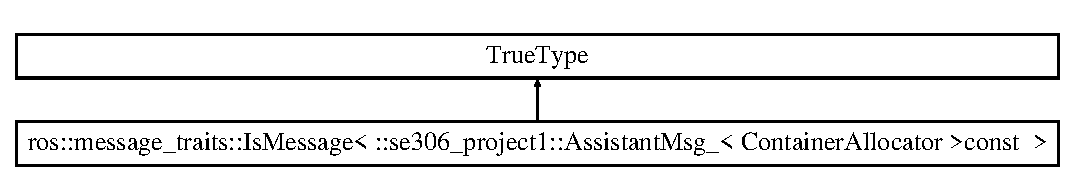
\includegraphics[height=1.992882cm]{structros_1_1message__traits_1_1IsMessage_3_01_1_1se306__project1_1_1AssistantMsg___3_01ContainerAllocator_01_4const_01_01_4}
\end{center}
\end{figure}


The documentation for this struct was generated from the following file\-:\begin{DoxyCompactItemize}
\item 
se306\-\_\-project1/msg\-\_\-gen/cpp/include/se306\-\_\-project1/Assistant\-Msg.\-h\end{DoxyCompactItemize}

\hypertarget{structros_1_1message__traits_1_1IsMessage_3_01_1_1se306__project1_1_1DoctorMsg___3_01ContainerAllocator_01_4_01_4}{\section{ros\-:\-:message\-\_\-traits\-:\-:Is\-Message$<$ \-:\-:se306\-\_\-project1\-:\-:Doctor\-Msg\-\_\-$<$ Container\-Allocator $>$ $>$ Struct Template Reference}
\label{structros_1_1message__traits_1_1IsMessage_3_01_1_1se306__project1_1_1DoctorMsg___3_01ContainerAllocator_01_4_01_4}\index{ros\-::message\-\_\-traits\-::\-Is\-Message$<$ \-::se306\-\_\-project1\-::\-Doctor\-Msg\-\_\-$<$ Container\-Allocator $>$ $>$@{ros\-::message\-\_\-traits\-::\-Is\-Message$<$ \-::se306\-\_\-project1\-::\-Doctor\-Msg\-\_\-$<$ Container\-Allocator $>$ $>$}}
}
Inheritance diagram for ros\-:\-:message\-\_\-traits\-:\-:Is\-Message$<$ \-:\-:se306\-\_\-project1\-:\-:Doctor\-Msg\-\_\-$<$ Container\-Allocator $>$ $>$\-:\begin{figure}[H]
\begin{center}
\leavevmode
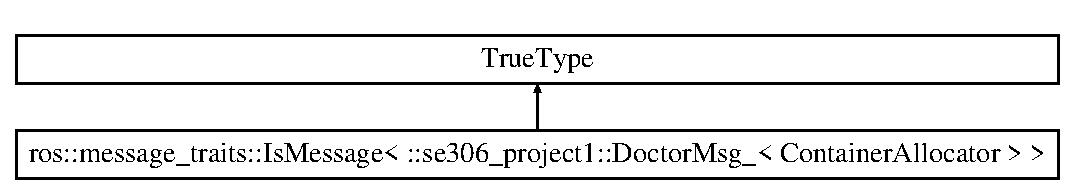
\includegraphics[height=2.000000cm]{structros_1_1message__traits_1_1IsMessage_3_01_1_1se306__project1_1_1DoctorMsg___3_01ContainerAllocator_01_4_01_4}
\end{center}
\end{figure}


The documentation for this struct was generated from the following file\-:\begin{DoxyCompactItemize}
\item 
se306\-\_\-project1/msg\-\_\-gen/cpp/include/se306\-\_\-project1/Doctor\-Msg.\-h\end{DoxyCompactItemize}

\hypertarget{structros_1_1message__traits_1_1IsMessage_3_01_1_1se306__project1_1_1DoctorMsg___3_01ContainerAllocator_01_4const_01_01_4}{\section{ros\-:\-:message\-\_\-traits\-:\-:Is\-Message$<$ \-:\-:se306\-\_\-project1\-:\-:Doctor\-Msg\-\_\-$<$ Container\-Allocator $>$const $>$ Struct Template Reference}
\label{structros_1_1message__traits_1_1IsMessage_3_01_1_1se306__project1_1_1DoctorMsg___3_01ContainerAllocator_01_4const_01_01_4}\index{ros\-::message\-\_\-traits\-::\-Is\-Message$<$ \-::se306\-\_\-project1\-::\-Doctor\-Msg\-\_\-$<$ Container\-Allocator $>$const  $>$@{ros\-::message\-\_\-traits\-::\-Is\-Message$<$ \-::se306\-\_\-project1\-::\-Doctor\-Msg\-\_\-$<$ Container\-Allocator $>$const  $>$}}
}
Inheritance diagram for ros\-:\-:message\-\_\-traits\-:\-:Is\-Message$<$ \-:\-:se306\-\_\-project1\-:\-:Doctor\-Msg\-\_\-$<$ Container\-Allocator $>$const $>$\-:\begin{figure}[H]
\begin{center}
\leavevmode
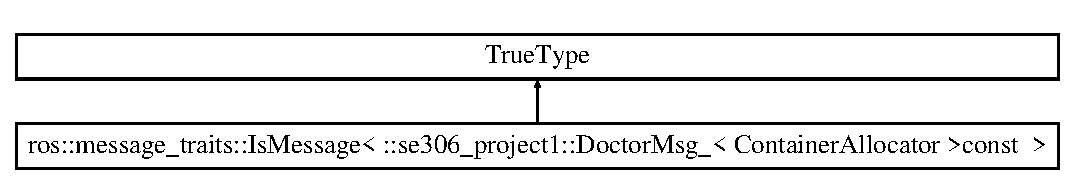
\includegraphics[height=2.000000cm]{structros_1_1message__traits_1_1IsMessage_3_01_1_1se306__project1_1_1DoctorMsg___3_01ContainerAllocator_01_4const_01_01_4}
\end{center}
\end{figure}


The documentation for this struct was generated from the following file\-:\begin{DoxyCompactItemize}
\item 
se306\-\_\-project1/msg\-\_\-gen/cpp/include/se306\-\_\-project1/Doctor\-Msg.\-h\end{DoxyCompactItemize}

\hypertarget{structros_1_1message__traits_1_1IsMessage_3_01_1_1se306__project1_1_1ResidentMsg___3_01ContainerAllocator_01_4_01_4}{\section{ros\-:\-:message\-\_\-traits\-:\-:Is\-Message$<$ \-:\-:se306\-\_\-project1\-:\-:Resident\-Msg\-\_\-$<$ Container\-Allocator $>$ $>$ Struct Template Reference}
\label{structros_1_1message__traits_1_1IsMessage_3_01_1_1se306__project1_1_1ResidentMsg___3_01ContainerAllocator_01_4_01_4}\index{ros\-::message\-\_\-traits\-::\-Is\-Message$<$ \-::se306\-\_\-project1\-::\-Resident\-Msg\-\_\-$<$ Container\-Allocator $>$ $>$@{ros\-::message\-\_\-traits\-::\-Is\-Message$<$ \-::se306\-\_\-project1\-::\-Resident\-Msg\-\_\-$<$ Container\-Allocator $>$ $>$}}
}
Inheritance diagram for ros\-:\-:message\-\_\-traits\-:\-:Is\-Message$<$ \-:\-:se306\-\_\-project1\-:\-:Resident\-Msg\-\_\-$<$ Container\-Allocator $>$ $>$\-:\begin{figure}[H]
\begin{center}
\leavevmode
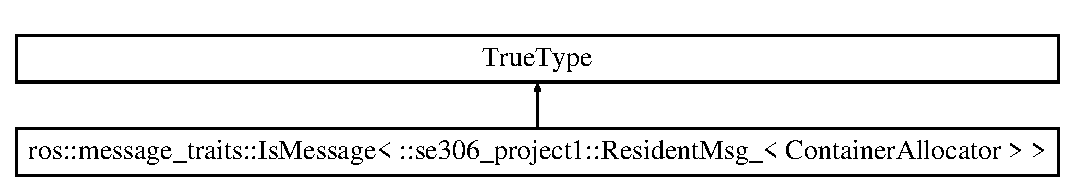
\includegraphics[height=2.000000cm]{structros_1_1message__traits_1_1IsMessage_3_01_1_1se306__project1_1_1ResidentMsg___3_01ContainerAllocator_01_4_01_4}
\end{center}
\end{figure}


The documentation for this struct was generated from the following file\-:\begin{DoxyCompactItemize}
\item 
se306\-\_\-project1/msg\-\_\-gen/cpp/include/se306\-\_\-project1/Resident\-Msg.\-h\end{DoxyCompactItemize}

\hypertarget{structros_1_1message__traits_1_1IsMessage_3_01_1_1se306__project1_1_1ResidentMsg___3_01ContainerAllocator_01_4const_01_01_4}{\section{ros\-:\-:message\-\_\-traits\-:\-:Is\-Message$<$ \-:\-:se306\-\_\-project1\-:\-:Resident\-Msg\-\_\-$<$ Container\-Allocator $>$const $>$ Struct Template Reference}
\label{structros_1_1message__traits_1_1IsMessage_3_01_1_1se306__project1_1_1ResidentMsg___3_01ContainerAllocator_01_4const_01_01_4}\index{ros\-::message\-\_\-traits\-::\-Is\-Message$<$ \-::se306\-\_\-project1\-::\-Resident\-Msg\-\_\-$<$ Container\-Allocator $>$const  $>$@{ros\-::message\-\_\-traits\-::\-Is\-Message$<$ \-::se306\-\_\-project1\-::\-Resident\-Msg\-\_\-$<$ Container\-Allocator $>$const  $>$}}
}
Inheritance diagram for ros\-:\-:message\-\_\-traits\-:\-:Is\-Message$<$ \-:\-:se306\-\_\-project1\-:\-:Resident\-Msg\-\_\-$<$ Container\-Allocator $>$const $>$\-:\begin{figure}[H]
\begin{center}
\leavevmode
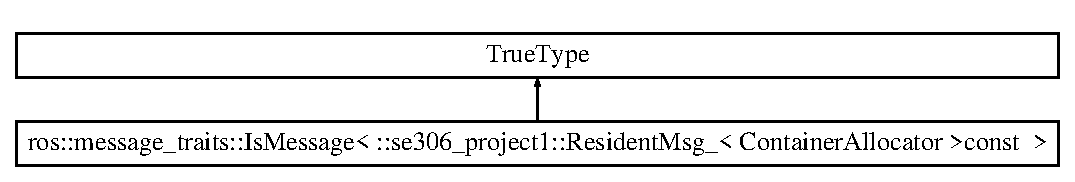
\includegraphics[height=2.000000cm]{structros_1_1message__traits_1_1IsMessage_3_01_1_1se306__project1_1_1ResidentMsg___3_01ContainerAllocator_01_4const_01_01_4}
\end{center}
\end{figure}


The documentation for this struct was generated from the following file\-:\begin{DoxyCompactItemize}
\item 
se306\-\_\-project1/msg\-\_\-gen/cpp/include/se306\-\_\-project1/Resident\-Msg.\-h\end{DoxyCompactItemize}

\hypertarget{structros_1_1message__traits_1_1MD5Sum_3_01_1_1se306__project1_1_1AssistantMsg___3_01ContainerAllocator_01_4_01_4}{\section{ros\-:\-:message\-\_\-traits\-:\-:M\-D5\-Sum$<$ \-:\-:se306\-\_\-project1\-:\-:Assistant\-Msg\-\_\-$<$ Container\-Allocator $>$ $>$ Struct Template Reference}
\label{structros_1_1message__traits_1_1MD5Sum_3_01_1_1se306__project1_1_1AssistantMsg___3_01ContainerAllocator_01_4_01_4}\index{ros\-::message\-\_\-traits\-::\-M\-D5\-Sum$<$ \-::se306\-\_\-project1\-::\-Assistant\-Msg\-\_\-$<$ Container\-Allocator $>$ $>$@{ros\-::message\-\_\-traits\-::\-M\-D5\-Sum$<$ \-::se306\-\_\-project1\-::\-Assistant\-Msg\-\_\-$<$ Container\-Allocator $>$ $>$}}
}
\subsection*{Static Public Member Functions}
\begin{DoxyCompactItemize}
\item 
\hypertarget{structros_1_1message__traits_1_1MD5Sum_3_01_1_1se306__project1_1_1AssistantMsg___3_01ContainerAllocator_01_4_01_4_a696176a6340716bab35810ff1ca89423}{static const char $\ast$ {\bfseries value} ()}\label{structros_1_1message__traits_1_1MD5Sum_3_01_1_1se306__project1_1_1AssistantMsg___3_01ContainerAllocator_01_4_01_4_a696176a6340716bab35810ff1ca89423}

\item 
\hypertarget{structros_1_1message__traits_1_1MD5Sum_3_01_1_1se306__project1_1_1AssistantMsg___3_01ContainerAllocator_01_4_01_4_a1d6448fa9fe928c2c9afcb0e564f975e}{static const char $\ast$ {\bfseries value} (const \-::\hyperlink{structse306__project1_1_1AssistantMsg__}{se306\-\_\-project1\-::\-Assistant\-Msg\-\_\-}$<$ Container\-Allocator $>$ \&)}\label{structros_1_1message__traits_1_1MD5Sum_3_01_1_1se306__project1_1_1AssistantMsg___3_01ContainerAllocator_01_4_01_4_a1d6448fa9fe928c2c9afcb0e564f975e}

\end{DoxyCompactItemize}
\subsection*{Static Public Attributes}
\begin{DoxyCompactItemize}
\item 
\hypertarget{structros_1_1message__traits_1_1MD5Sum_3_01_1_1se306__project1_1_1AssistantMsg___3_01ContainerAllocator_01_4_01_4_a2fe2af80ffa1a7473555eecfa65f5bdb}{static const uint64\-\_\-t {\bfseries static\-\_\-value1} = 0xa03c5f8f468a7475\-U\-L\-L}\label{structros_1_1message__traits_1_1MD5Sum_3_01_1_1se306__project1_1_1AssistantMsg___3_01ContainerAllocator_01_4_01_4_a2fe2af80ffa1a7473555eecfa65f5bdb}

\item 
\hypertarget{structros_1_1message__traits_1_1MD5Sum_3_01_1_1se306__project1_1_1AssistantMsg___3_01ContainerAllocator_01_4_01_4_ae6d40a1d0327b6d042044884fb350544}{static const uint64\-\_\-t {\bfseries static\-\_\-value2} = 0xee423369456ec01c\-U\-L\-L}\label{structros_1_1message__traits_1_1MD5Sum_3_01_1_1se306__project1_1_1AssistantMsg___3_01ContainerAllocator_01_4_01_4_ae6d40a1d0327b6d042044884fb350544}

\end{DoxyCompactItemize}


The documentation for this struct was generated from the following file\-:\begin{DoxyCompactItemize}
\item 
se306\-\_\-project1/msg\-\_\-gen/cpp/include/se306\-\_\-project1/Assistant\-Msg.\-h\end{DoxyCompactItemize}

\hypertarget{structros_1_1message__traits_1_1MD5Sum_3_01_1_1se306__project1_1_1DoctorMsg___3_01ContainerAllocator_01_4_01_4}{\section{ros\-:\-:message\-\_\-traits\-:\-:M\-D5\-Sum$<$ \-:\-:se306\-\_\-project1\-:\-:Doctor\-Msg\-\_\-$<$ Container\-Allocator $>$ $>$ Struct Template Reference}
\label{structros_1_1message__traits_1_1MD5Sum_3_01_1_1se306__project1_1_1DoctorMsg___3_01ContainerAllocator_01_4_01_4}\index{ros\-::message\-\_\-traits\-::\-M\-D5\-Sum$<$ \-::se306\-\_\-project1\-::\-Doctor\-Msg\-\_\-$<$ Container\-Allocator $>$ $>$@{ros\-::message\-\_\-traits\-::\-M\-D5\-Sum$<$ \-::se306\-\_\-project1\-::\-Doctor\-Msg\-\_\-$<$ Container\-Allocator $>$ $>$}}
}
\subsection*{Static Public Member Functions}
\begin{DoxyCompactItemize}
\item 
\hypertarget{structros_1_1message__traits_1_1MD5Sum_3_01_1_1se306__project1_1_1DoctorMsg___3_01ContainerAllocator_01_4_01_4_a5f3b0909336db6fd963a5c764264336c}{static const char $\ast$ {\bfseries value} ()}\label{structros_1_1message__traits_1_1MD5Sum_3_01_1_1se306__project1_1_1DoctorMsg___3_01ContainerAllocator_01_4_01_4_a5f3b0909336db6fd963a5c764264336c}

\item 
\hypertarget{structros_1_1message__traits_1_1MD5Sum_3_01_1_1se306__project1_1_1DoctorMsg___3_01ContainerAllocator_01_4_01_4_a022fb5d69dca3e28f1d49ccf25d85755}{static const char $\ast$ {\bfseries value} (const \-::\hyperlink{structse306__project1_1_1DoctorMsg__}{se306\-\_\-project1\-::\-Doctor\-Msg\-\_\-}$<$ Container\-Allocator $>$ \&)}\label{structros_1_1message__traits_1_1MD5Sum_3_01_1_1se306__project1_1_1DoctorMsg___3_01ContainerAllocator_01_4_01_4_a022fb5d69dca3e28f1d49ccf25d85755}

\end{DoxyCompactItemize}
\subsection*{Static Public Attributes}
\begin{DoxyCompactItemize}
\item 
\hypertarget{structros_1_1message__traits_1_1MD5Sum_3_01_1_1se306__project1_1_1DoctorMsg___3_01ContainerAllocator_01_4_01_4_a82ad2a2715ca706b4df782355a581377}{static const uint64\-\_\-t {\bfseries static\-\_\-value1} = 0xadcd587ba691a57f\-U\-L\-L}\label{structros_1_1message__traits_1_1MD5Sum_3_01_1_1se306__project1_1_1DoctorMsg___3_01ContainerAllocator_01_4_01_4_a82ad2a2715ca706b4df782355a581377}

\item 
\hypertarget{structros_1_1message__traits_1_1MD5Sum_3_01_1_1se306__project1_1_1DoctorMsg___3_01ContainerAllocator_01_4_01_4_ac439ab233b91d5252db5d305e83f8231}{static const uint64\-\_\-t {\bfseries static\-\_\-value2} = 0xd4852480ac57651e\-U\-L\-L}\label{structros_1_1message__traits_1_1MD5Sum_3_01_1_1se306__project1_1_1DoctorMsg___3_01ContainerAllocator_01_4_01_4_ac439ab233b91d5252db5d305e83f8231}

\end{DoxyCompactItemize}


The documentation for this struct was generated from the following file\-:\begin{DoxyCompactItemize}
\item 
se306\-\_\-project1/msg\-\_\-gen/cpp/include/se306\-\_\-project1/Doctor\-Msg.\-h\end{DoxyCompactItemize}

\hypertarget{structros_1_1message__traits_1_1MD5Sum_3_01_1_1se306__project1_1_1ResidentMsg___3_01ContainerAllocator_01_4_01_4}{\section{ros\-:\-:message\-\_\-traits\-:\-:M\-D5\-Sum$<$ \-:\-:se306\-\_\-project1\-:\-:Resident\-Msg\-\_\-$<$ Container\-Allocator $>$ $>$ Struct Template Reference}
\label{structros_1_1message__traits_1_1MD5Sum_3_01_1_1se306__project1_1_1ResidentMsg___3_01ContainerAllocator_01_4_01_4}\index{ros\-::message\-\_\-traits\-::\-M\-D5\-Sum$<$ \-::se306\-\_\-project1\-::\-Resident\-Msg\-\_\-$<$ Container\-Allocator $>$ $>$@{ros\-::message\-\_\-traits\-::\-M\-D5\-Sum$<$ \-::se306\-\_\-project1\-::\-Resident\-Msg\-\_\-$<$ Container\-Allocator $>$ $>$}}
}
\subsection*{Static Public Member Functions}
\begin{DoxyCompactItemize}
\item 
\hypertarget{structros_1_1message__traits_1_1MD5Sum_3_01_1_1se306__project1_1_1ResidentMsg___3_01ContainerAllocator_01_4_01_4_a4b4e542d789bbf861e057e4b92121eba}{static const char $\ast$ {\bfseries value} ()}\label{structros_1_1message__traits_1_1MD5Sum_3_01_1_1se306__project1_1_1ResidentMsg___3_01ContainerAllocator_01_4_01_4_a4b4e542d789bbf861e057e4b92121eba}

\item 
\hypertarget{structros_1_1message__traits_1_1MD5Sum_3_01_1_1se306__project1_1_1ResidentMsg___3_01ContainerAllocator_01_4_01_4_ae56825e64f6dba43dbd980a0696c277b}{static const char $\ast$ {\bfseries value} (const \-::\hyperlink{structse306__project1_1_1ResidentMsg__}{se306\-\_\-project1\-::\-Resident\-Msg\-\_\-}$<$ Container\-Allocator $>$ \&)}\label{structros_1_1message__traits_1_1MD5Sum_3_01_1_1se306__project1_1_1ResidentMsg___3_01ContainerAllocator_01_4_01_4_ae56825e64f6dba43dbd980a0696c277b}

\end{DoxyCompactItemize}
\subsection*{Static Public Attributes}
\begin{DoxyCompactItemize}
\item 
\hypertarget{structros_1_1message__traits_1_1MD5Sum_3_01_1_1se306__project1_1_1ResidentMsg___3_01ContainerAllocator_01_4_01_4_a37972fc33e3a5f7f44d6e783d452d689}{static const uint64\-\_\-t {\bfseries static\-\_\-value1} = 0xd4a55c59ae8655ae\-U\-L\-L}\label{structros_1_1message__traits_1_1MD5Sum_3_01_1_1se306__project1_1_1ResidentMsg___3_01ContainerAllocator_01_4_01_4_a37972fc33e3a5f7f44d6e783d452d689}

\item 
\hypertarget{structros_1_1message__traits_1_1MD5Sum_3_01_1_1se306__project1_1_1ResidentMsg___3_01ContainerAllocator_01_4_01_4_a83dba0321612123fae5b2a20ccaa2aee}{static const uint64\-\_\-t {\bfseries static\-\_\-value2} = 0x9644ee9979fbb7c9\-U\-L\-L}\label{structros_1_1message__traits_1_1MD5Sum_3_01_1_1se306__project1_1_1ResidentMsg___3_01ContainerAllocator_01_4_01_4_a83dba0321612123fae5b2a20ccaa2aee}

\end{DoxyCompactItemize}


The documentation for this struct was generated from the following file\-:\begin{DoxyCompactItemize}
\item 
se306\-\_\-project1/msg\-\_\-gen/cpp/include/se306\-\_\-project1/Resident\-Msg.\-h\end{DoxyCompactItemize}

\hypertarget{classNurse}{\section{Nurse Class Reference}
\label{classNurse}\index{Nurse@{Nurse}}
}


Class for \hyperlink{classNurse}{Nurse} nodes.  




{\ttfamily \#include $<$Nurse.\-h$>$}

Inheritance diagram for Nurse\-:\begin{figure}[H]
\begin{center}
\leavevmode
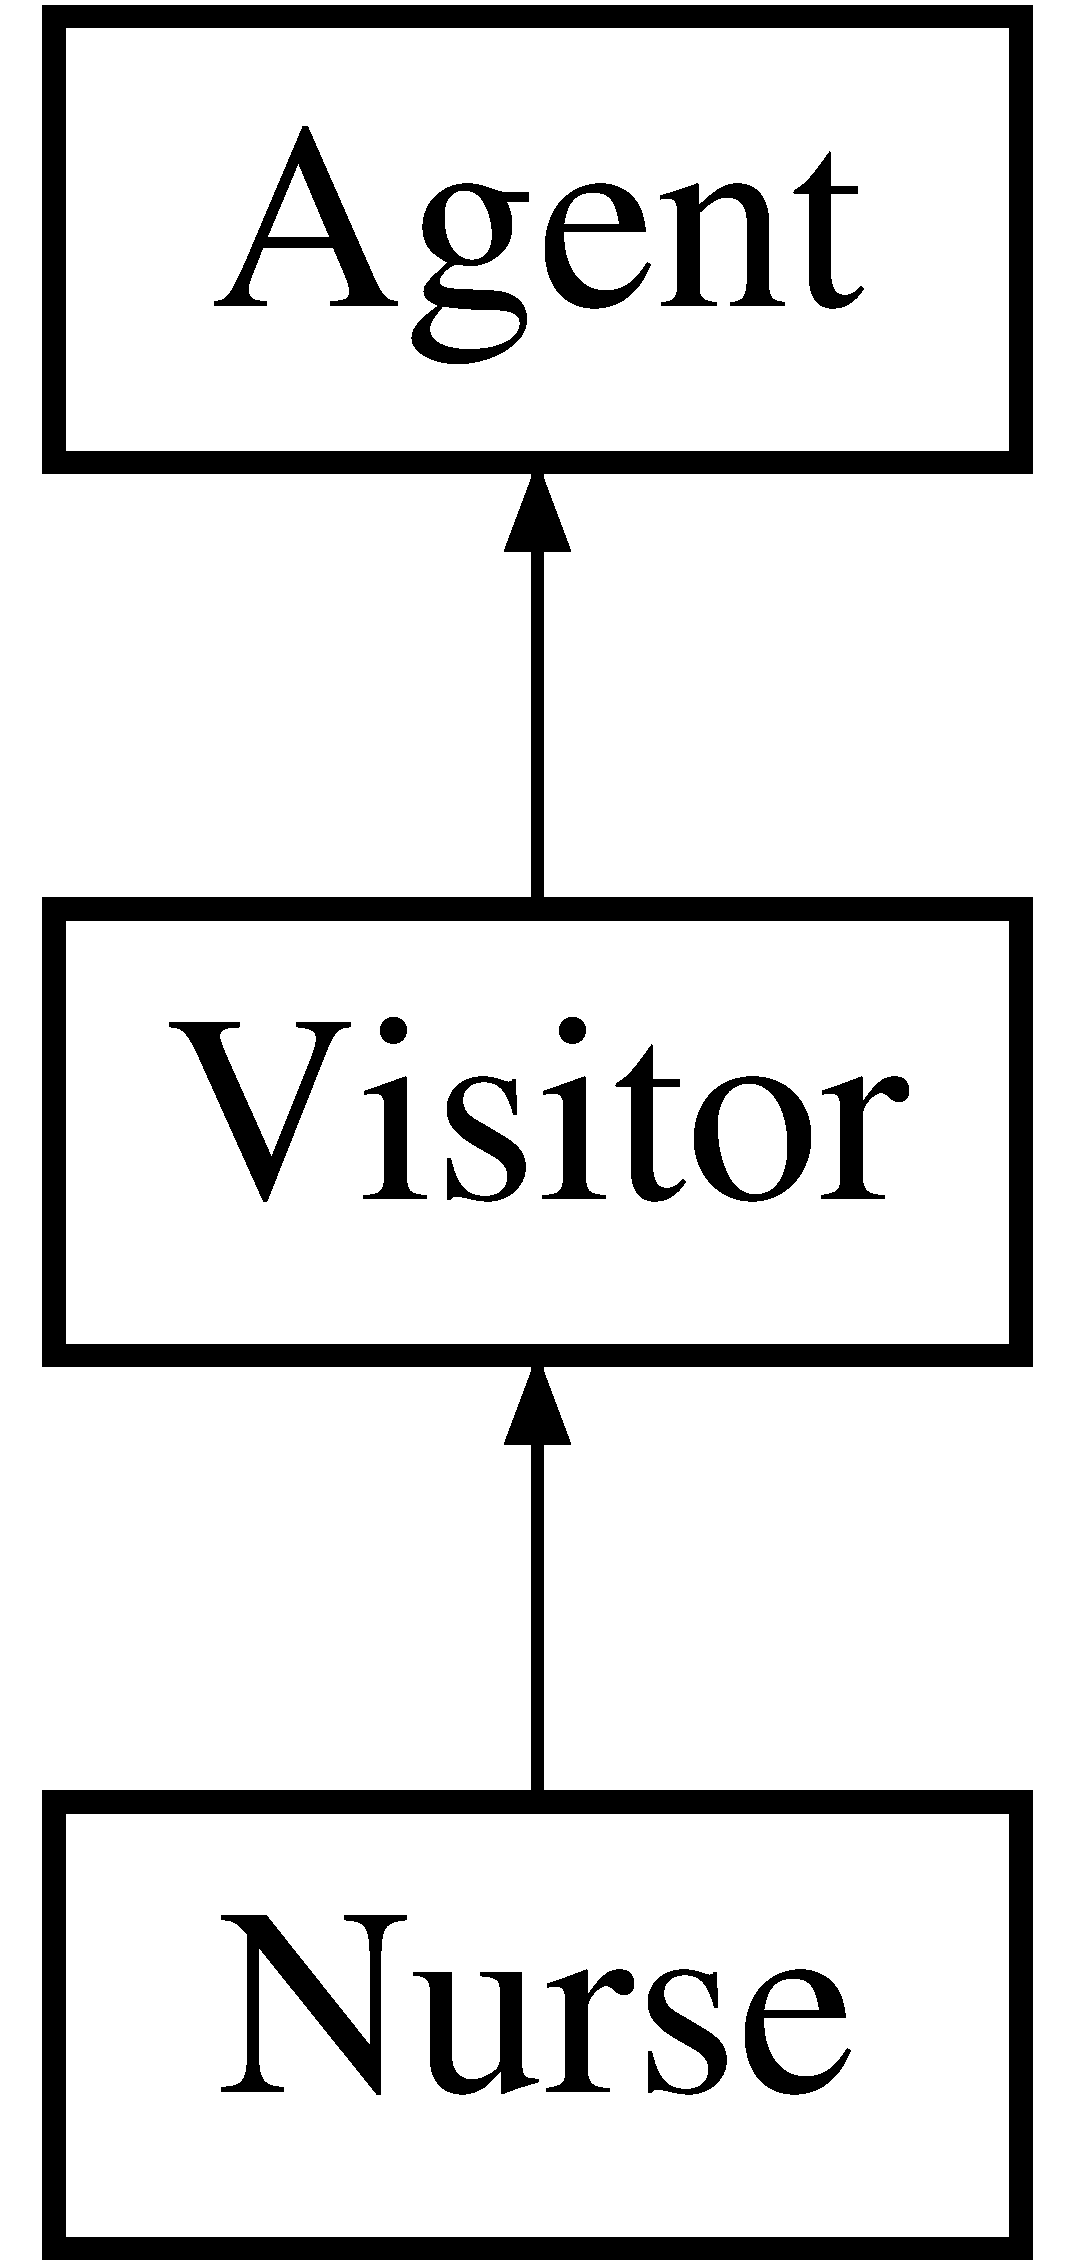
\includegraphics[height=3.000000cm]{classNurse}
\end{center}
\end{figure}
\subsection*{Public Member Functions}
\begin{DoxyCompactItemize}
\item 
\hypertarget{classNurse_ab58da68573cbe6f62dab9298acfd6ba6}{int \hyperlink{classNurse_ab58da68573cbe6f62dab9298acfd6ba6}{run} (int argc, char $\ast$argv\mbox{[}$\,$\mbox{]})}\label{classNurse_ab58da68573cbe6f62dab9298acfd6ba6}

\begin{DoxyCompactList}\small\item\em Main function for the \hyperlink{classNurse}{Nurse} process. Controls node setup and periodic events. \end{DoxyCompactList}\end{DoxyCompactItemize}
\subsection*{Protected Member Functions}
\begin{DoxyCompactItemize}
\item 
\hypertarget{classNurse_aa84201e0e9fd8628847a720f74de68b5}{void \hyperlink{classNurse_aa84201e0e9fd8628847a720f74de68b5}{do\-Hospitalise} ()}\label{classNurse_aa84201e0e9fd8628847a720f74de68b5}

\begin{DoxyCompactList}\small\item\em Takes the resident to hospital (non-\/doctor-\/induced emergency, despite the function name...) \end{DoxyCompactList}\item 
void \hyperlink{classNurse_a5791a1e191c2025b0a7d3522fe101f64}{delegate} (\hyperlink{structse306__project1_1_1ResidentMsg__}{se306\-\_\-project1\-::\-Resident\-Msg} msg)
\begin{DoxyCompactList}\small\item\em Callback function that unpacks and processes resident status messages. \hyperlink{classNurse}{Nurse} should subscribe to the Resident\-Msg topic in order for this callback to be called. Resident\-Msg is published by the \hyperlink{classResident}{Resident}. \end{DoxyCompactList}\end{DoxyCompactItemize}
\subsection*{Additional Inherited Members}


\subsection{Detailed Description}
Class for \hyperlink{classNurse}{Nurse} nodes. 

\subsection{Member Function Documentation}
\hypertarget{classNurse_a5791a1e191c2025b0a7d3522fe101f64}{\index{Nurse@{Nurse}!delegate@{delegate}}
\index{delegate@{delegate}!Nurse@{Nurse}}
\subsubsection[{delegate}]{\setlength{\rightskip}{0pt plus 5cm}void Nurse\-::delegate (
\begin{DoxyParamCaption}
\item[{{\bf se306\-\_\-project1\-::\-Resident\-Msg}}]{msg}
\end{DoxyParamCaption}
)\hspace{0.3cm}{\ttfamily [protected]}}}\label{classNurse_a5791a1e191c2025b0a7d3522fe101f64}


Callback function that unpacks and processes resident status messages. \hyperlink{classNurse}{Nurse} should subscribe to the Resident\-Msg topic in order for this callback to be called. Resident\-Msg is published by the \hyperlink{classResident}{Resident}. 


\begin{DoxyParams}{Parameters}
{\em msg} & A custom Resident\-Msg message that contains information about the resident's current status. \\
\hline
\end{DoxyParams}


The documentation for this class was generated from the following files\-:\begin{DoxyCompactItemize}
\item 
se306\-\_\-project1/src/Nurse.\-h\item 
se306\-\_\-project1/src/Nurse.\-cpp\end{DoxyCompactItemize}

\hypertarget{classNurse1}{\section{Nurse1 Class Reference}
\label{classNurse1}\index{Nurse1@{Nurse1}}
}


Class for \hyperlink{classNurse}{Nurse} nodes.  




{\ttfamily \#include $<$Nurse1.\-h$>$}

Inheritance diagram for Nurse1\-:\begin{figure}[H]
\begin{center}
\leavevmode
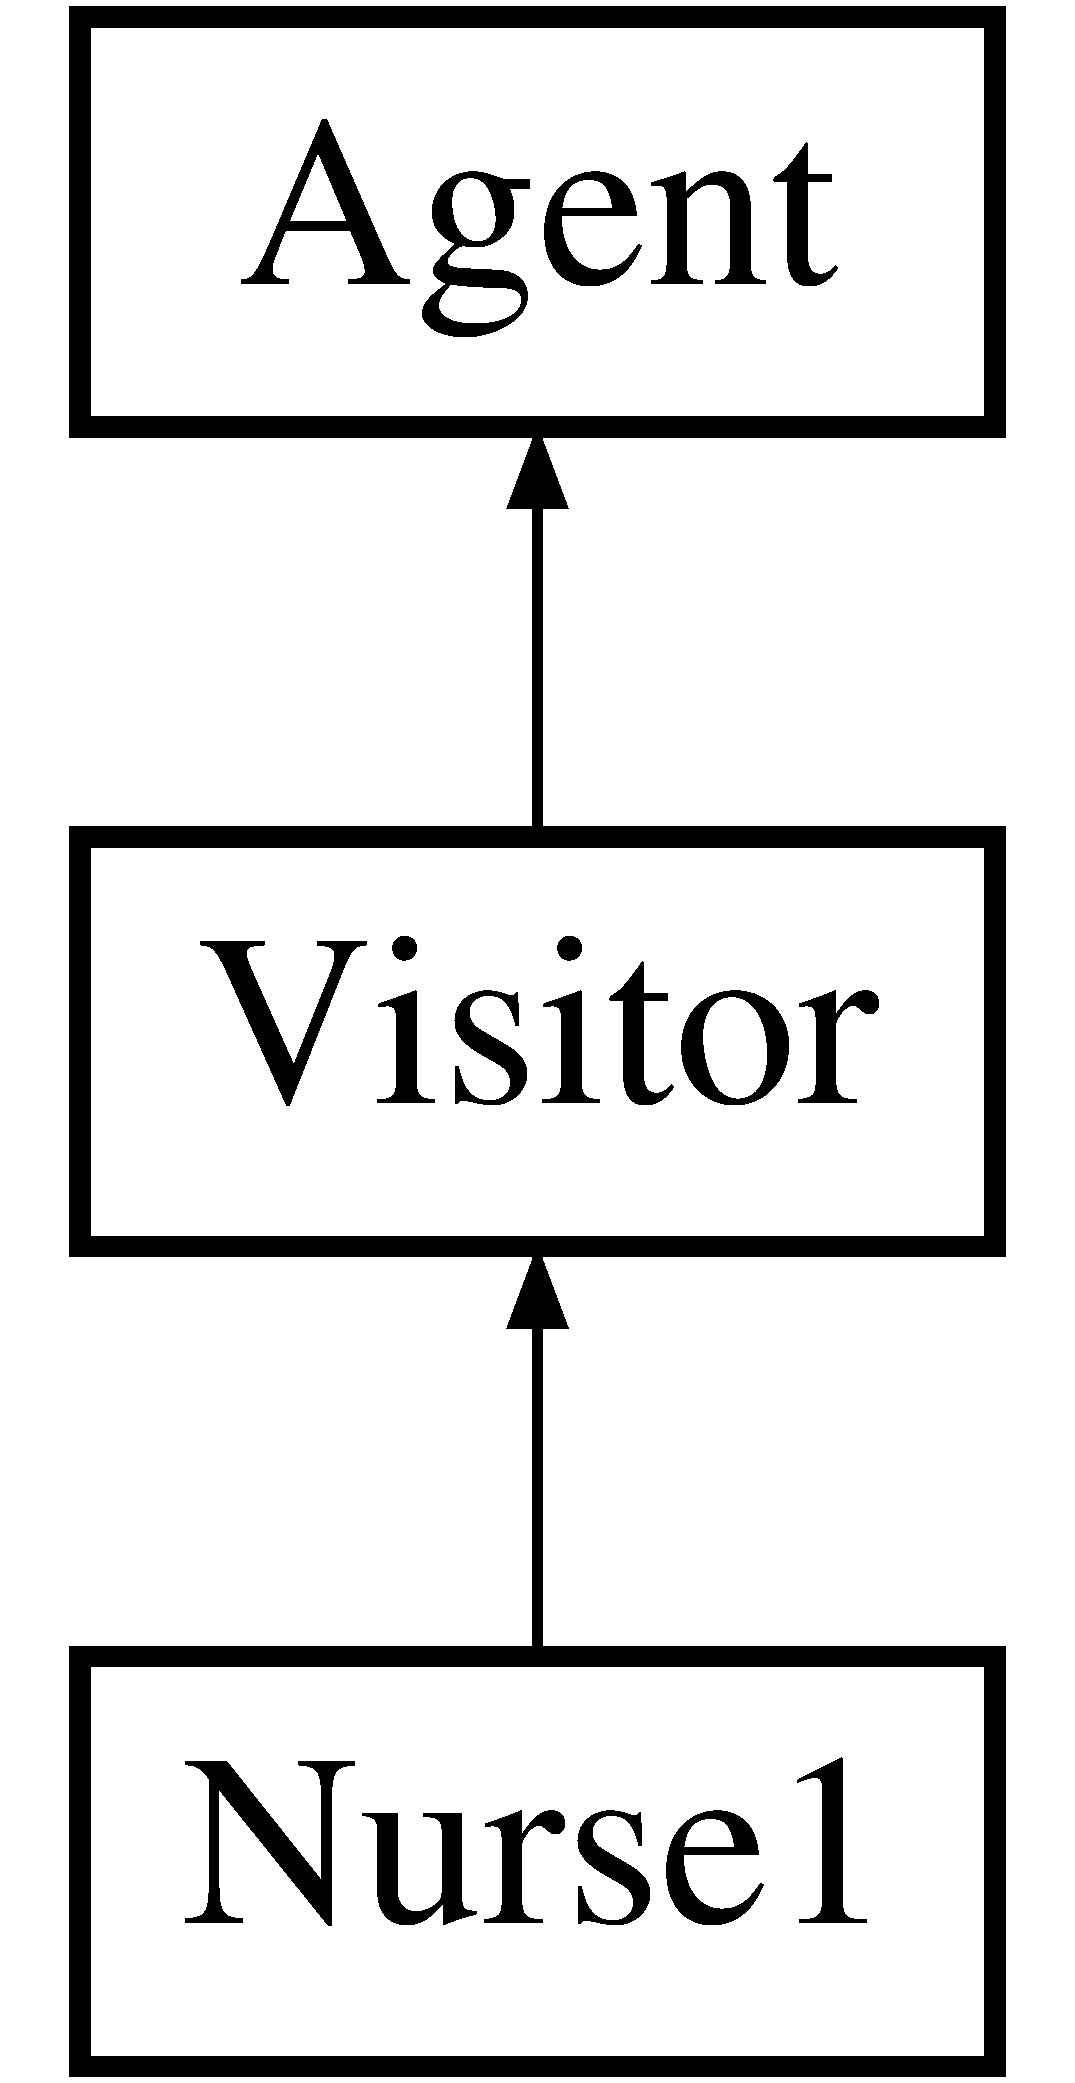
\includegraphics[height=3.000000cm]{classNurse1}
\end{center}
\end{figure}
\subsection*{Public Member Functions}
\begin{DoxyCompactItemize}
\item 
\hypertarget{classNurse1_aa886de90970d5c54832808c3b6fdef0d}{int \hyperlink{classNurse1_aa886de90970d5c54832808c3b6fdef0d}{run} (int argc, char $\ast$argv\mbox{[}$\,$\mbox{]})}\label{classNurse1_aa886de90970d5c54832808c3b6fdef0d}

\begin{DoxyCompactList}\small\item\em Main function for the \hyperlink{classNurse}{Nurse} process. Controls node setup and periodic events. \end{DoxyCompactList}\end{DoxyCompactItemize}
\subsection*{Protected Member Functions}
\begin{DoxyCompactItemize}
\item 
\hypertarget{classNurse1_a87357493032169a577c1845c42cd3236}{void \hyperlink{classNurse1_a87357493032169a577c1845c42cd3236}{do\-Hospitalise} (\hyperlink{structse306__project1_1_1ResidentMsg__}{se306\-\_\-project1\-::\-Resident\-Msg} msg)}\label{classNurse1_a87357493032169a577c1845c42cd3236}

\begin{DoxyCompactList}\small\item\em Takes the resident to hospital (non-\/doctor-\/induced emergency, despite the function name...) \end{DoxyCompactList}\item 
void \hyperlink{classNurse1_ac95056e8cc50a59564a67e8a4f3cd5c7}{delegate} (\hyperlink{structse306__project1_1_1ResidentMsg__}{se306\-\_\-project1\-::\-Resident\-Msg} msg)
\begin{DoxyCompactList}\small\item\em Callback function that unpacks and processes resident status messages. \hyperlink{classNurse}{Nurse} should subscribe to the Resident\-Msg topic in order for this callback to be called. Resident\-Msg is published by the \hyperlink{classResident}{Resident}. \end{DoxyCompactList}\end{DoxyCompactItemize}
\subsection*{Additional Inherited Members}


\subsection{Detailed Description}
Class for \hyperlink{classNurse}{Nurse} nodes. 

\subsection{Member Function Documentation}
\hypertarget{classNurse1_ac95056e8cc50a59564a67e8a4f3cd5c7}{\index{Nurse1@{Nurse1}!delegate@{delegate}}
\index{delegate@{delegate}!Nurse1@{Nurse1}}
\subsubsection[{delegate}]{\setlength{\rightskip}{0pt plus 5cm}void Nurse1\-::delegate (
\begin{DoxyParamCaption}
\item[{{\bf se306\-\_\-project1\-::\-Resident\-Msg}}]{msg}
\end{DoxyParamCaption}
)\hspace{0.3cm}{\ttfamily [protected]}}}\label{classNurse1_ac95056e8cc50a59564a67e8a4f3cd5c7}


Callback function that unpacks and processes resident status messages. \hyperlink{classNurse}{Nurse} should subscribe to the Resident\-Msg topic in order for this callback to be called. Resident\-Msg is published by the \hyperlink{classResident}{Resident}. 


\begin{DoxyParams}{Parameters}
{\em msg} & A custom Resident\-Msg message that contains information about the resident's current status. \\
\hline
\end{DoxyParams}


The documentation for this class was generated from the following files\-:\begin{DoxyCompactItemize}
\item 
se306\-\_\-project1/src/Nurse1.\-h\item 
se306\-\_\-project1/src/Nurse1.\-cpp\end{DoxyCompactItemize}

\hypertarget{classNurse2}{\section{Nurse2 Class Reference}
\label{classNurse2}\index{Nurse2@{Nurse2}}
}


Class for \hyperlink{classNurse}{Nurse} nodes.  




{\ttfamily \#include $<$Nurse2.\-h$>$}

Inheritance diagram for Nurse2\-:\begin{figure}[H]
\begin{center}
\leavevmode
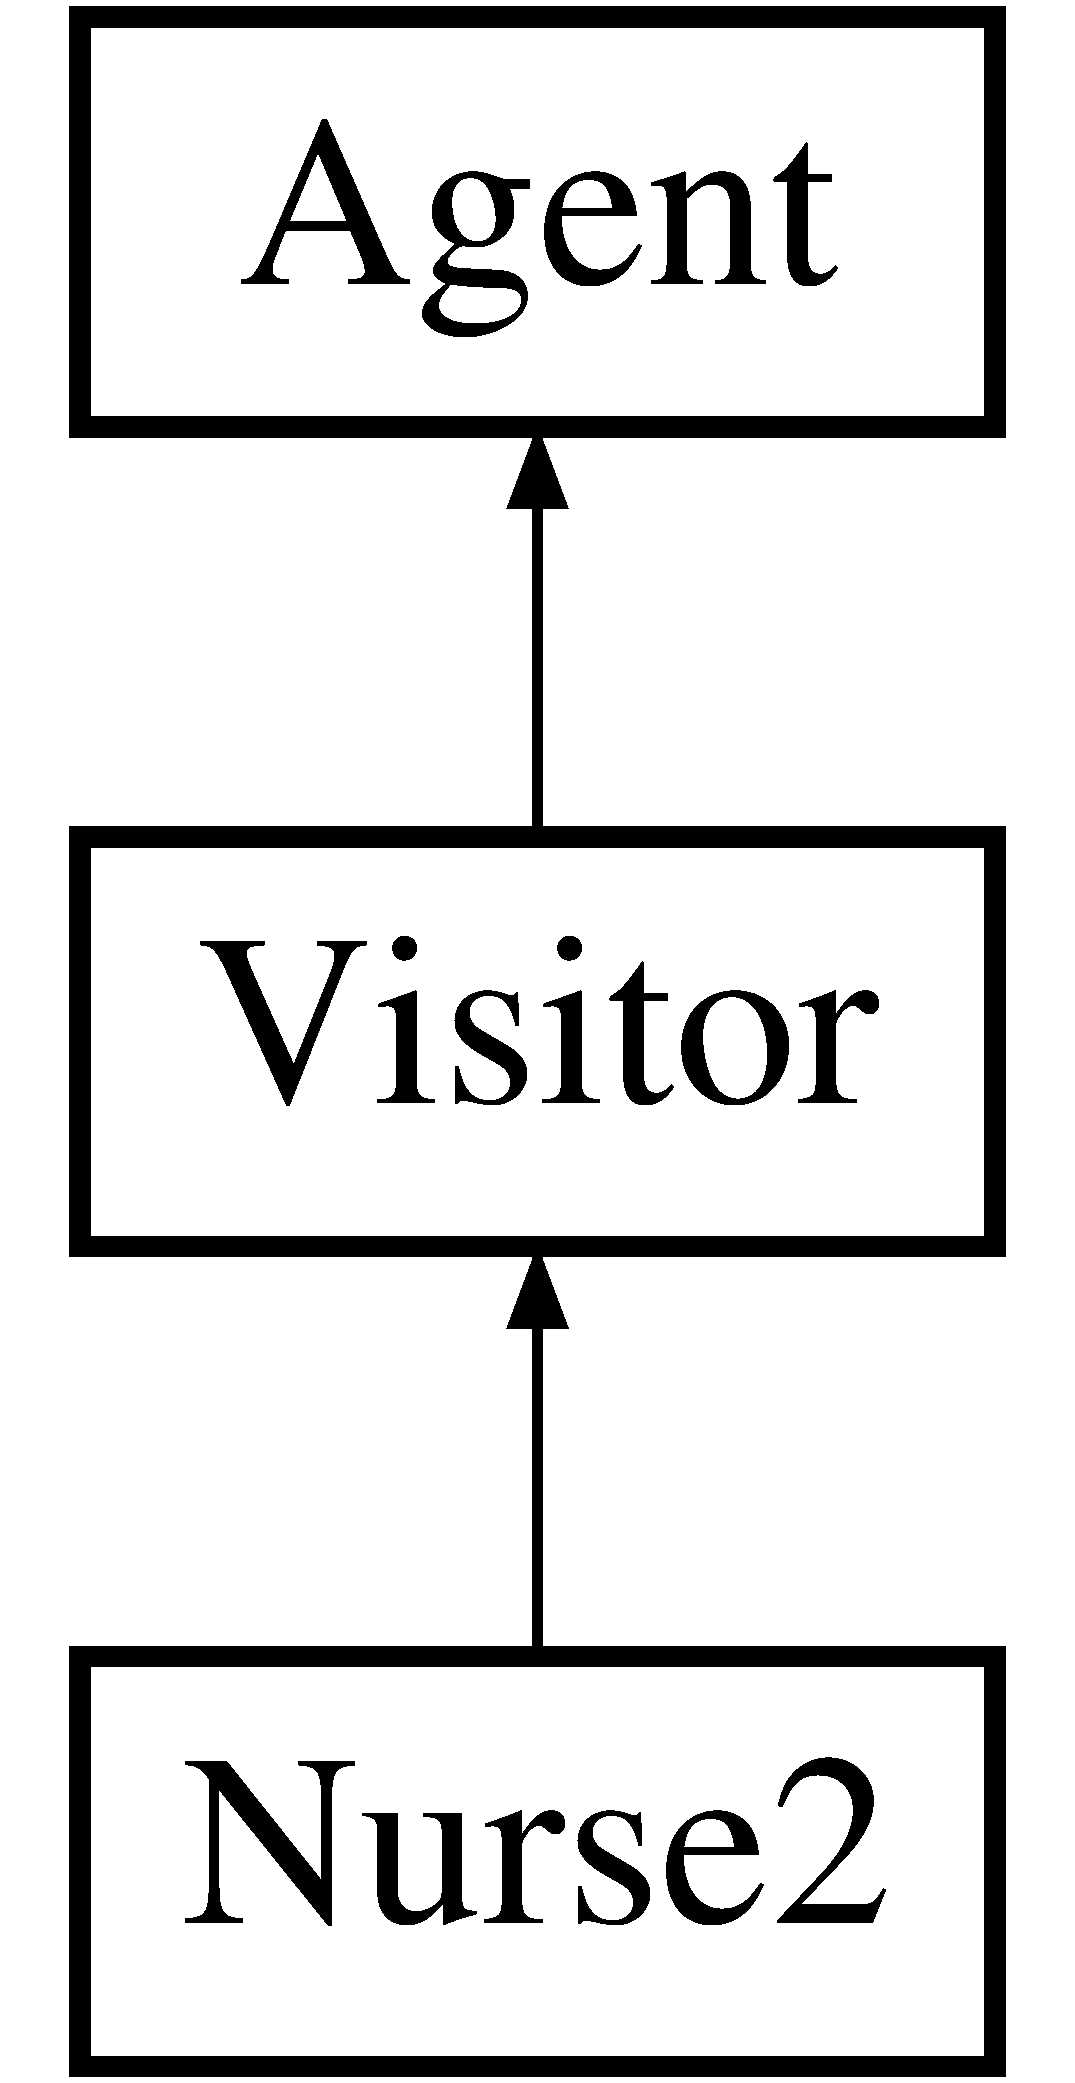
\includegraphics[height=3.000000cm]{classNurse2}
\end{center}
\end{figure}
\subsection*{Public Member Functions}
\begin{DoxyCompactItemize}
\item 
\hypertarget{classNurse2_a5f7eae9d158eb137b5fcb465c84d1c82}{int \hyperlink{classNurse2_a5f7eae9d158eb137b5fcb465c84d1c82}{run} (int argc, char $\ast$argv\mbox{[}$\,$\mbox{]})}\label{classNurse2_a5f7eae9d158eb137b5fcb465c84d1c82}

\begin{DoxyCompactList}\small\item\em Main function for the \hyperlink{classNurse}{Nurse} process. Controls node setup and periodic events. \end{DoxyCompactList}\end{DoxyCompactItemize}
\subsection*{Protected Member Functions}
\begin{DoxyCompactItemize}
\item 
\hypertarget{classNurse2_a506228f056abb95488c436d3440c6119}{void \hyperlink{classNurse2_a506228f056abb95488c436d3440c6119}{do\-Hospitalise} (\hyperlink{structse306__project1_1_1ResidentMsg__}{se306\-\_\-project1\-::\-Resident\-Msg} msg)}\label{classNurse2_a506228f056abb95488c436d3440c6119}

\begin{DoxyCompactList}\small\item\em Takes the resident to hospital (non-\/doctor-\/induced emergency, despite the function name...) \end{DoxyCompactList}\item 
void \hyperlink{classNurse2_a97b9ad49242153b9d1d35ef6e4c88dd6}{delegate} (\hyperlink{structse306__project1_1_1ResidentMsg__}{se306\-\_\-project1\-::\-Resident\-Msg} msg)
\begin{DoxyCompactList}\small\item\em Callback function that unpacks and processes resident status messages. \hyperlink{classNurse}{Nurse} should subscribe to the Resident\-Msg topic in order for this callback to be called. Resident\-Msg is published by the \hyperlink{classResident}{Resident}. \end{DoxyCompactList}\end{DoxyCompactItemize}
\subsection*{Additional Inherited Members}


\subsection{Detailed Description}
Class for \hyperlink{classNurse}{Nurse} nodes. 

\subsection{Member Function Documentation}
\hypertarget{classNurse2_a97b9ad49242153b9d1d35ef6e4c88dd6}{\index{Nurse2@{Nurse2}!delegate@{delegate}}
\index{delegate@{delegate}!Nurse2@{Nurse2}}
\subsubsection[{delegate}]{\setlength{\rightskip}{0pt plus 5cm}void Nurse2\-::delegate (
\begin{DoxyParamCaption}
\item[{{\bf se306\-\_\-project1\-::\-Resident\-Msg}}]{msg}
\end{DoxyParamCaption}
)\hspace{0.3cm}{\ttfamily [protected]}}}\label{classNurse2_a97b9ad49242153b9d1d35ef6e4c88dd6}


Callback function that unpacks and processes resident status messages. \hyperlink{classNurse}{Nurse} should subscribe to the Resident\-Msg topic in order for this callback to be called. Resident\-Msg is published by the \hyperlink{classResident}{Resident}. 


\begin{DoxyParams}{Parameters}
{\em msg} & A custom Resident\-Msg message that contains information about the resident's current status. \\
\hline
\end{DoxyParams}


The documentation for this class was generated from the following files\-:\begin{DoxyCompactItemize}
\item 
se306\-\_\-project1/src/Nurse2.\-h\item 
se306\-\_\-project1/src/Nurse2.\-cpp\end{DoxyCompactItemize}

\hypertarget{structros_1_1message__operations_1_1Printer_3_01_1_1se306__project1_1_1AssistantMsg___3_01ContainerAllocator_01_4_01_4}{\section{ros\-:\-:message\-\_\-operations\-:\-:Printer$<$ \-:\-:se306\-\_\-project1\-:\-:Assistant\-Msg\-\_\-$<$ Container\-Allocator $>$ $>$ Struct Template Reference}
\label{structros_1_1message__operations_1_1Printer_3_01_1_1se306__project1_1_1AssistantMsg___3_01ContainerAllocator_01_4_01_4}\index{ros\-::message\-\_\-operations\-::\-Printer$<$ \-::se306\-\_\-project1\-::\-Assistant\-Msg\-\_\-$<$ Container\-Allocator $>$ $>$@{ros\-::message\-\_\-operations\-::\-Printer$<$ \-::se306\-\_\-project1\-::\-Assistant\-Msg\-\_\-$<$ Container\-Allocator $>$ $>$}}
}
\subsection*{Static Public Member Functions}
\begin{DoxyCompactItemize}
\item 
\hypertarget{structros_1_1message__operations_1_1Printer_3_01_1_1se306__project1_1_1AssistantMsg___3_01ContainerAllocator_01_4_01_4_afbf2d719d6d838e543faa7109287651f}{{\footnotesize template$<$typename Stream $>$ }\\static void {\bfseries stream} (Stream \&s, const std\-::string \&indent, const \-::\hyperlink{structse306__project1_1_1AssistantMsg__}{se306\-\_\-project1\-::\-Assistant\-Msg\-\_\-}$<$ Container\-Allocator $>$ \&v)}\label{structros_1_1message__operations_1_1Printer_3_01_1_1se306__project1_1_1AssistantMsg___3_01ContainerAllocator_01_4_01_4_afbf2d719d6d838e543faa7109287651f}

\end{DoxyCompactItemize}


The documentation for this struct was generated from the following file\-:\begin{DoxyCompactItemize}
\item 
se306\-\_\-project1/msg\-\_\-gen/cpp/include/se306\-\_\-project1/Assistant\-Msg.\-h\end{DoxyCompactItemize}

\hypertarget{structros_1_1message__operations_1_1Printer_3_01_1_1se306__project1_1_1DoctorMsg___3_01ContainerAllocator_01_4_01_4}{\section{ros\-:\-:message\-\_\-operations\-:\-:Printer$<$ \-:\-:se306\-\_\-project1\-:\-:Doctor\-Msg\-\_\-$<$ Container\-Allocator $>$ $>$ Struct Template Reference}
\label{structros_1_1message__operations_1_1Printer_3_01_1_1se306__project1_1_1DoctorMsg___3_01ContainerAllocator_01_4_01_4}\index{ros\-::message\-\_\-operations\-::\-Printer$<$ \-::se306\-\_\-project1\-::\-Doctor\-Msg\-\_\-$<$ Container\-Allocator $>$ $>$@{ros\-::message\-\_\-operations\-::\-Printer$<$ \-::se306\-\_\-project1\-::\-Doctor\-Msg\-\_\-$<$ Container\-Allocator $>$ $>$}}
}
\subsection*{Static Public Member Functions}
\begin{DoxyCompactItemize}
\item 
\hypertarget{structros_1_1message__operations_1_1Printer_3_01_1_1se306__project1_1_1DoctorMsg___3_01ContainerAllocator_01_4_01_4_a9edb461075970680eda73a334f371cc5}{{\footnotesize template$<$typename Stream $>$ }\\static void {\bfseries stream} (Stream \&s, const std\-::string \&indent, const \-::\hyperlink{structse306__project1_1_1DoctorMsg__}{se306\-\_\-project1\-::\-Doctor\-Msg\-\_\-}$<$ Container\-Allocator $>$ \&v)}\label{structros_1_1message__operations_1_1Printer_3_01_1_1se306__project1_1_1DoctorMsg___3_01ContainerAllocator_01_4_01_4_a9edb461075970680eda73a334f371cc5}

\end{DoxyCompactItemize}


The documentation for this struct was generated from the following file\-:\begin{DoxyCompactItemize}
\item 
se306\-\_\-project1/msg\-\_\-gen/cpp/include/se306\-\_\-project1/Doctor\-Msg.\-h\end{DoxyCompactItemize}

\hypertarget{structros_1_1message__operations_1_1Printer_3_01_1_1se306__project1_1_1ResidentMsg___3_01ContainerAllocator_01_4_01_4}{\section{ros\-:\-:message\-\_\-operations\-:\-:Printer$<$ \-:\-:se306\-\_\-project1\-:\-:Resident\-Msg\-\_\-$<$ Container\-Allocator $>$ $>$ Struct Template Reference}
\label{structros_1_1message__operations_1_1Printer_3_01_1_1se306__project1_1_1ResidentMsg___3_01ContainerAllocator_01_4_01_4}\index{ros\-::message\-\_\-operations\-::\-Printer$<$ \-::se306\-\_\-project1\-::\-Resident\-Msg\-\_\-$<$ Container\-Allocator $>$ $>$@{ros\-::message\-\_\-operations\-::\-Printer$<$ \-::se306\-\_\-project1\-::\-Resident\-Msg\-\_\-$<$ Container\-Allocator $>$ $>$}}
}
\subsection*{Static Public Member Functions}
\begin{DoxyCompactItemize}
\item 
\hypertarget{structros_1_1message__operations_1_1Printer_3_01_1_1se306__project1_1_1ResidentMsg___3_01ContainerAllocator_01_4_01_4_aa2309bcca506e2bef9cbc8b0d6e7e36a}{{\footnotesize template$<$typename Stream $>$ }\\static void {\bfseries stream} (Stream \&s, const std\-::string \&indent, const \-::\hyperlink{structse306__project1_1_1ResidentMsg__}{se306\-\_\-project1\-::\-Resident\-Msg\-\_\-}$<$ Container\-Allocator $>$ \&v)}\label{structros_1_1message__operations_1_1Printer_3_01_1_1se306__project1_1_1ResidentMsg___3_01ContainerAllocator_01_4_01_4_aa2309bcca506e2bef9cbc8b0d6e7e36a}

\end{DoxyCompactItemize}


The documentation for this struct was generated from the following file\-:\begin{DoxyCompactItemize}
\item 
se306\-\_\-project1/msg\-\_\-gen/cpp/include/se306\-\_\-project1/Resident\-Msg.\-h\end{DoxyCompactItemize}

\hypertarget{classpriorityQueue}{\section{priority\-Queue Class Reference}
\label{classpriorityQueue}\index{priority\-Queue@{priority\-Queue}}
}
\subsection*{Public Member Functions}
\begin{DoxyCompactItemize}
\item 
\hypertarget{classpriorityQueue_a58658233e429bf3666dc4eb5300012c4}{void {\bfseries add\-To\-P\-Q} (resident\-States current\-State)}\label{classpriorityQueue_a58658233e429bf3666dc4eb5300012c4}

\item 
\hypertarget{classpriorityQueue_a78d5b85232d7303cabc49c4fac41a0ec}{resident\-States {\bfseries pop\-From\-P\-Q} ()}\label{classpriorityQueue_a78d5b85232d7303cabc49c4fac41a0ec}

\item 
\hypertarget{classpriorityQueue_a1d4923612653d4b3f810b7451d21004d}{std\-::string {\bfseries check\-Current\-State} ()}\label{classpriorityQueue_a1d4923612653d4b3f810b7451d21004d}

\item 
\hypertarget{classpriorityQueue_a448eafd83ae7742c21b8f70b078ae48b}{void {\bfseries remove\-State} (resident\-States unwanted\-State)}\label{classpriorityQueue_a448eafd83ae7742c21b8f70b078ae48b}

\end{DoxyCompactItemize}


The documentation for this class was generated from the following files\-:\begin{DoxyCompactItemize}
\item 
se306\-\_\-project1/src/priority\-Queue.\-h\item 
se306\-\_\-project1/src/priority\-Queue.\-cpp\end{DoxyCompactItemize}

\hypertarget{classProcessManager}{\section{Process\-Manager Class Reference}
\label{classProcessManager}\index{Process\-Manager@{Process\-Manager}}
}


Class for managing node processes. Should keep track of nodes and be able to instantiate them.  




{\ttfamily \#include $<$Process\-Manager.\-h$>$}

\subsection*{Public Member Functions}
\begin{DoxyCompactItemize}
\item 
\hypertarget{classProcessManager_ac551563da6cc98d4639a6724372815ef}{int {\bfseries node\-Process} (std\-::string executable\-Name, int node\-Number)}\label{classProcessManager_ac551563da6cc98d4639a6724372815ef}

\end{DoxyCompactItemize}


\subsection{Detailed Description}
Class for managing node processes. Should keep track of nodes and be able to instantiate them. 

The documentation for this class was generated from the following files\-:\begin{DoxyCompactItemize}
\item 
se306\-\_\-project1/src/Process\-Manager.\-h\item 
se306\-\_\-project1/src/Process\-Manager.\-cpp\end{DoxyCompactItemize}

\hypertarget{classRelative}{\section{Relative Class Reference}
\label{classRelative}\index{Relative@{Relative}}
}


Class for \hyperlink{classRelative}{Relative} nodes.  




{\ttfamily \#include $<$Relative.\-h$>$}

Inheritance diagram for Relative\-:\begin{figure}[H]
\begin{center}
\leavevmode
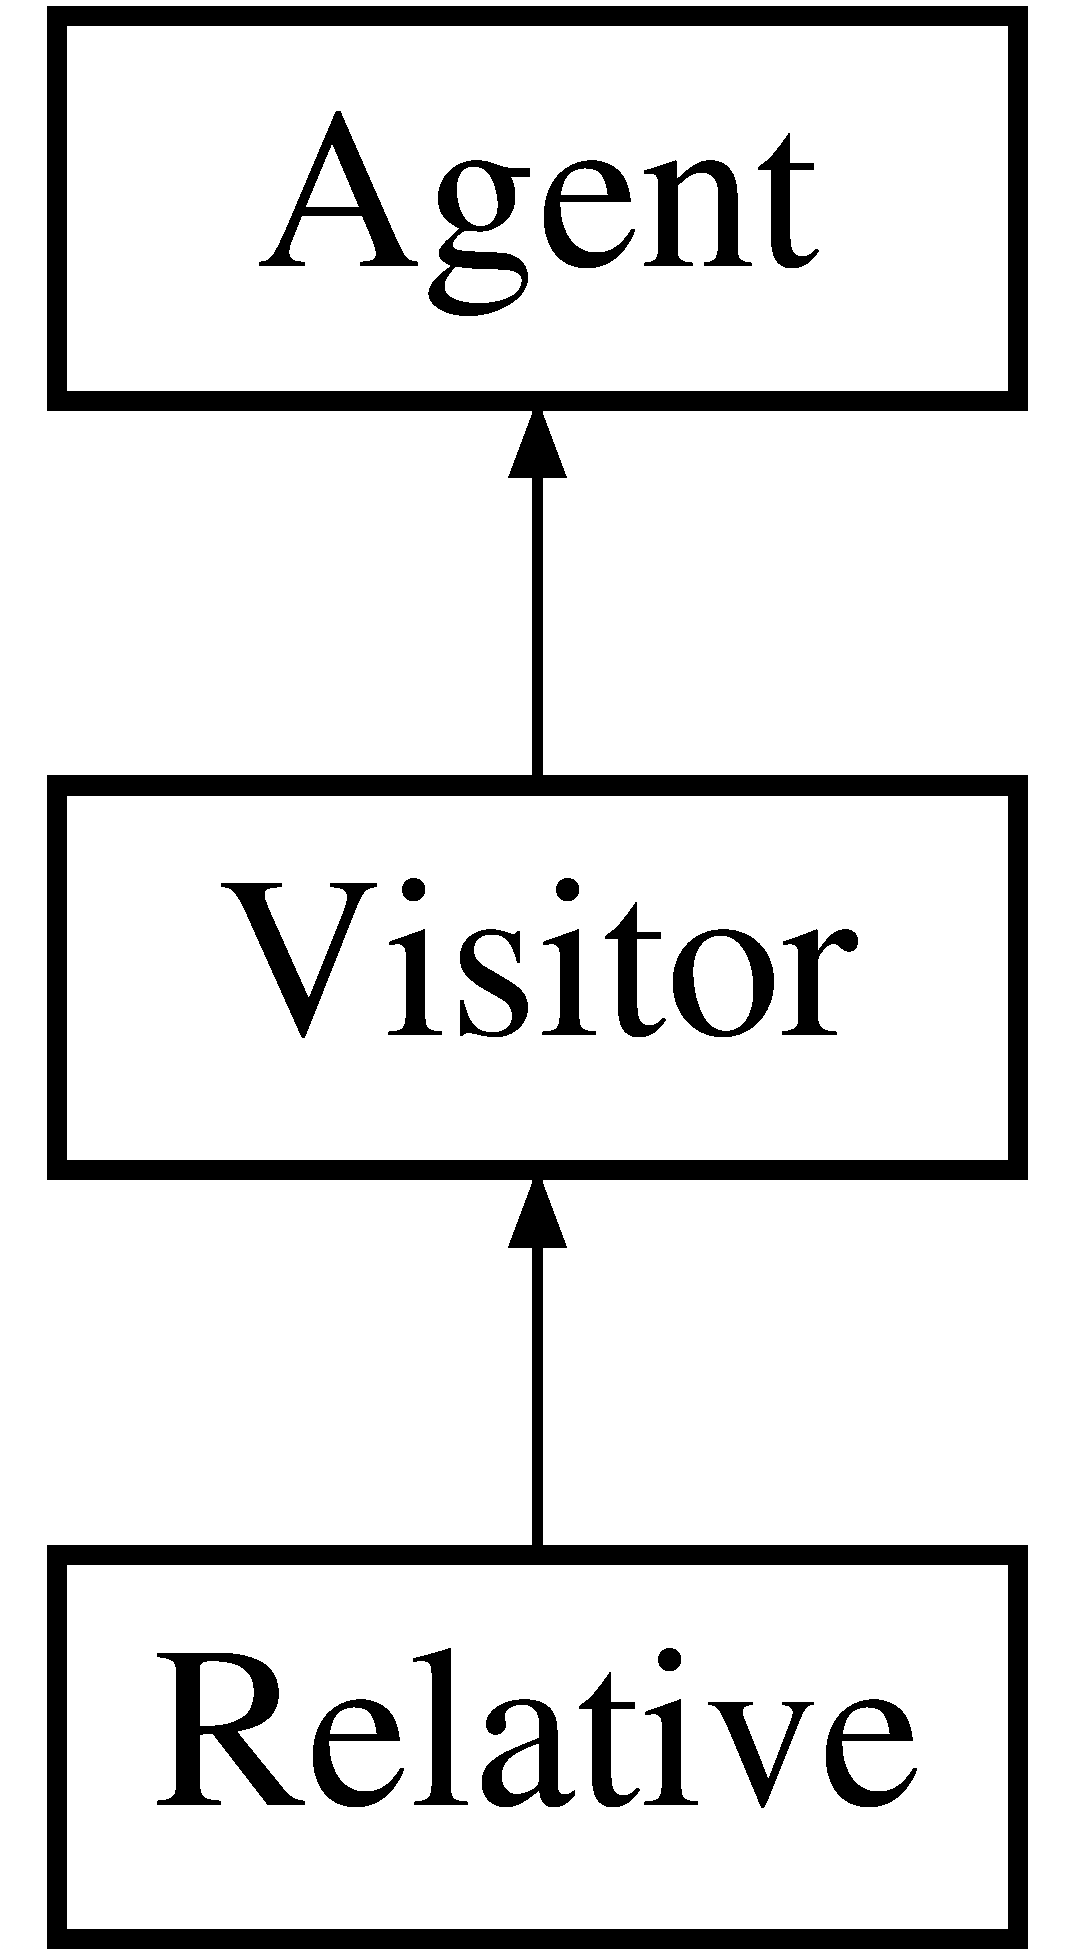
\includegraphics[height=3.000000cm]{classRelative}
\end{center}
\end{figure}
\subsection*{Public Member Functions}
\begin{DoxyCompactItemize}
\item 
void \hyperlink{classRelative_a13fc6c65f7338cfa29c9f31958134c56}{Stage\-Odom\-\_\-callback} (nav\-\_\-msgs\-::\-Odometry msg)
\begin{DoxyCompactList}\small\item\em Updates the \hyperlink{classRelative}{Relative}'s x position, y position, and angle to reflect its current pose. \end{DoxyCompactList}\item 
void \hyperlink{classRelative_a556d177e5d1562ab9af5018ef382c836}{Stage\-Laser\-\_\-callback} (sensor\-\_\-msgs\-::\-Laser\-Scan msg)
\begin{DoxyCompactList}\small\item\em Callback function to process laser scan messsages. You can access the range data from msg.\-ranges\mbox{[}i\mbox{]}. i = sample number. \end{DoxyCompactList}\item 
\hypertarget{classRelative_a966fc1a728e7b4ab9bde0cb636b5d7a9}{int \hyperlink{classRelative_a966fc1a728e7b4ab9bde0cb636b5d7a9}{run} (int argc, char $\ast$$\ast$argv)}\label{classRelative_a966fc1a728e7b4ab9bde0cb636b5d7a9}

\begin{DoxyCompactList}\small\item\em Main function for the \hyperlink{classRelative}{Relative} process. Controls node setup and periodic events. \end{DoxyCompactList}\end{DoxyCompactItemize}
\subsection*{Additional Inherited Members}


\subsection{Detailed Description}
Class for \hyperlink{classRelative}{Relative} nodes. 

\subsection{Member Function Documentation}
\hypertarget{classRelative_a556d177e5d1562ab9af5018ef382c836}{\index{Relative@{Relative}!Stage\-Laser\-\_\-callback@{Stage\-Laser\-\_\-callback}}
\index{Stage\-Laser\-\_\-callback@{Stage\-Laser\-\_\-callback}!Relative@{Relative}}
\subsubsection[{Stage\-Laser\-\_\-callback}]{\setlength{\rightskip}{0pt plus 5cm}void Relative\-::\-Stage\-Laser\-\_\-callback (
\begin{DoxyParamCaption}
\item[{sensor\-\_\-msgs\-::\-Laser\-Scan}]{msg}
\end{DoxyParamCaption}
)\hspace{0.3cm}{\ttfamily [virtual]}}}\label{classRelative_a556d177e5d1562ab9af5018ef382c836}


Callback function to process laser scan messsages. You can access the range data from msg.\-ranges\mbox{[}i\mbox{]}. i = sample number. 

\begin{DoxyNote}{Note}
Currently blank as it is not in use. Navigation operates through a checkpoint system. 
\end{DoxyNote}

\begin{DoxyParams}{Parameters}
{\em msg} & Single scan from a planar laser range finder \\
\hline
\end{DoxyParams}


Implements \hyperlink{classAgent_adfe1de8bbeaa7e4a5f7f2ff3e45593e8}{Agent}.

\hypertarget{classRelative_a13fc6c65f7338cfa29c9f31958134c56}{\index{Relative@{Relative}!Stage\-Odom\-\_\-callback@{Stage\-Odom\-\_\-callback}}
\index{Stage\-Odom\-\_\-callback@{Stage\-Odom\-\_\-callback}!Relative@{Relative}}
\subsubsection[{Stage\-Odom\-\_\-callback}]{\setlength{\rightskip}{0pt plus 5cm}void Relative\-::\-Stage\-Odom\-\_\-callback (
\begin{DoxyParamCaption}
\item[{nav\-\_\-msgs\-::\-Odometry}]{msg}
\end{DoxyParamCaption}
)\hspace{0.3cm}{\ttfamily [virtual]}}}\label{classRelative_a13fc6c65f7338cfa29c9f31958134c56}


Updates the \hyperlink{classRelative}{Relative}'s x position, y position, and angle to reflect its current pose. 

\begin{DoxyNote}{Note}
Rounding is used to calculate the current angle. This approximation is accounted for by using threshholds when processing angles. 
\end{DoxyNote}

\begin{DoxyParams}{Parameters}
{\em msg} & Odometry message from odom topic \\
\hline
\end{DoxyParams}


Implements \hyperlink{classAgent_a4b1182b9ee5dccaa871d71beef94a7d2}{Agent}.



The documentation for this class was generated from the following files\-:\begin{DoxyCompactItemize}
\item 
se306\-\_\-project1/src/Relative.\-h\item 
se306\-\_\-project1/src/Relative.\-cpp\end{DoxyCompactItemize}

\hypertarget{classResident}{\section{Resident Class Reference}
\label{classResident}\index{Resident@{Resident}}
}


Class representing the \hyperlink{classResident}{Resident}.  




{\ttfamily \#include $<$Resident.\-h$>$}

Inheritance diagram for Resident\-:\begin{figure}[H]
\begin{center}
\leavevmode
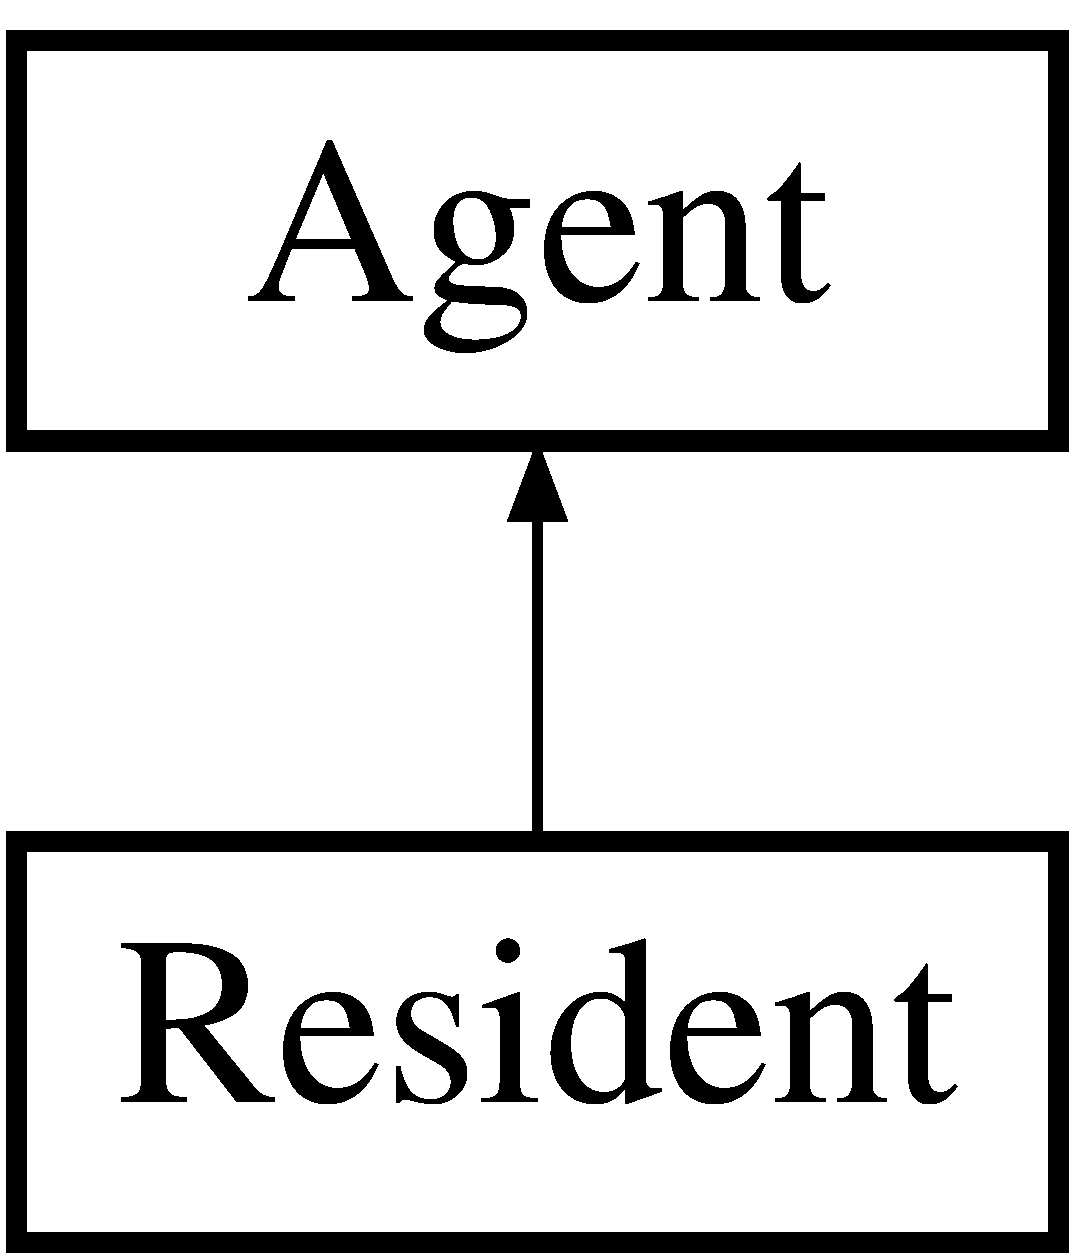
\includegraphics[height=2.000000cm]{classResident}
\end{center}
\end{figure}
\subsection*{Public Member Functions}
\begin{DoxyCompactItemize}
\item 
void \hyperlink{classResident_ae1406a27c978147c7816e57f9ed13aed}{Stage\-Odom\-\_\-callback} (nav\-\_\-msgs\-::\-Odometry msg)
\begin{DoxyCompactList}\small\item\em Updates the \hyperlink{classResident}{Resident}'s x position, y position, and angle to reflect its current pose. \end{DoxyCompactList}\item 
void \hyperlink{classResident_a6745ec218b7e451eb7ba2ca88fa2aca9}{Stage\-Laser\-\_\-callback} (sensor\-\_\-msgs\-::\-Laser\-Scan msg)
\begin{DoxyCompactList}\small\item\em Callback function to process laser scan messsages. You can access the range data from msg.\-ranges\mbox{[}i\mbox{]}. i = sample number. \end{DoxyCompactList}\item 
\hypertarget{classResident_aa4cbafa8f6cf586b53a774a8f1d81aa6}{int \hyperlink{classResident_aa4cbafa8f6cf586b53a774a8f1d81aa6}{run} (int argc, char $\ast$$\ast$argv) = checkpoints\mbox{[}cc-\/1\mbox{]}\mbox{[}0\mbox{]}}\label{classResident_aa4cbafa8f6cf586b53a774a8f1d81aa6}

\begin{DoxyCompactList}\small\item\em Main function for the \hyperlink{classResident}{Resident} process. Controls node setup and periodic events. \end{DoxyCompactList}\item 
void \hyperlink{classResident_a6d8fbbc8a60508ec913fb41d7e743094}{doctor\-\_\-callback} (\hyperlink{structse306__project1_1_1DoctorMsg__}{se306\-\_\-project1\-::\-Doctor\-Msg} msg)
\begin{DoxyCompactList}\small\item\em Increases the resident's health when the doctor heals them. \end{DoxyCompactList}\item 
double \hyperlink{classResident_ae8e00862499c8a502b5c99f8267d3345}{calc\-\_\-goal\-\_\-angle} (double \hyperlink{classResident_adee57a6649dfa4a41d027fbb8d961226}{goal\-\_\-x}, double \hyperlink{classResident_a30e28a999b67c4db3500c9c3c9989a10}{goal\-\_\-y}, double \hyperlink{classResident_a4781565db7a2e58566d2120623fbc13e}{cur\-\_\-angle}, double \hyperlink{classResident_aa147b3e473b2ea32b732eb5146ec7e34}{px}, double \hyperlink{classResident_ac757cac74a1712dd5746d1c3f5702a21}{py})
\begin{DoxyCompactList}\small\item\em Given the agent's current angle, this function calculates the angle to the goal. cur\-\_\-angle, goal\-\_\-x, goal\-\_\-y, px, and py are class fields but are also passed as parameters. \end{DoxyCompactList}\item 
std\-::pair$<$ double, double $>$ \hyperlink{classResident_a6f48fd57a638a2b4599777a1be766296}{move} (double \hyperlink{classResident_adee57a6649dfa4a41d027fbb8d961226}{goal\-\_\-x}, double \hyperlink{classResident_a30e28a999b67c4db3500c9c3c9989a10}{goal\-\_\-y}, double \hyperlink{classResident_a4781565db7a2e58566d2120623fbc13e}{cur\-\_\-angle}, double \hyperlink{classResident_a194117576f1937cac43ac1b05b884085}{goal\-\_\-angle}, double \hyperlink{classResident_aa147b3e473b2ea32b732eb5146ec7e34}{px}, double \hyperlink{classResident_ac757cac74a1712dd5746d1c3f5702a21}{py})
\begin{DoxyCompactList}\small\item\em Keeps the agent moving by changing linear\-\_\-x ad angular\-\_\-z. \end{DoxyCompactList}\item 
\hypertarget{classResident_a538db1d9cce0d967a78e7d10876d76ca}{void {\bfseries random\-Checkpoint\-Callback} (const ros\-::\-Timer\-Event \&)}\label{classResident_a538db1d9cce0d967a78e7d10876d76ca}

\item 
void \hyperlink{classResident_aa715d491e917de6f621593f0d1f01bd6}{assistant\-\_\-callback} (\hyperlink{structse306__project1_1_1AssistantMsg__}{se306\-\_\-project1\-::\-Assistant\-Msg} msg)
\begin{DoxyCompactList}\small\item\em Increases the \hyperlink{classResident}{Resident}'s hunger (towards full) if food has been delivered. \end{DoxyCompactList}\item 
std\-::pair$<$ double, double $>$ \hyperlink{classResident_a0cfe1d9b185beed7d3438157cc69db05}{move\-Path} (int path\mbox{[}$\,$\mbox{]}\mbox{[}2\mbox{]}, int path\-Length)
\begin{DoxyCompactList}\small\item\em Causes the agent to move until the goal is reached. When the goal is reached, the next checkpoint becomes the goal or if the list of checkpoints is exhausted, the agent returns to its initial position (the first checkpoint) \end{DoxyCompactList}\end{DoxyCompactItemize}
\subsection*{Protected Attributes}
\begin{DoxyCompactItemize}
\item 
int \hyperlink{classResident_ac603d9684120e1ab66a4340797bb7e90}{health}
\item 
int \hyperlink{classResident_acc61e75ef963ee7a6945b4d2ae9c55e6}{boredom}
\item 
int \hyperlink{classResident_a337df4272a4640a4039dfbe5c5c4a6d6}{hunger}
\item 
double \hyperlink{classResident_adee57a6649dfa4a41d027fbb8d961226}{goal\-\_\-x}
\item 
double \hyperlink{classResident_a30e28a999b67c4db3500c9c3c9989a10}{goal\-\_\-y}
\item 
double \hyperlink{classResident_aa147b3e473b2ea32b732eb5146ec7e34}{px}
\item 
double \hyperlink{classResident_ac757cac74a1712dd5746d1c3f5702a21}{py}
\item 
double \hyperlink{classResident_a194117576f1937cac43ac1b05b884085}{goal\-\_\-angle}
\item 
bool \hyperlink{classResident_ac5e7527b191e07372c3ea5e9aa81a65d}{is\-Set}
\item 
double \hyperlink{classResident_a4781565db7a2e58566d2120623fbc13e}{cur\-\_\-angle}
\item 
\hypertarget{classResident_ab17c0dfd1b011b6e166f987f823892da}{int {\bfseries cc}}\label{classResident_ab17c0dfd1b011b6e166f987f823892da}

\item 
\hypertarget{classResident_aa2c1d458eb7b852af9aaa39132e0d85a}{bool {\bfseries is\-\_\-called}}\label{classResident_aa2c1d458eb7b852af9aaa39132e0d85a}

\item 
\hypertarget{classResident_af86d17339240199486745bdd27da0ca5}{std\-::pair$<$ double, bool $>$ {\bfseries goal\-\_\-pair}}\label{classResident_af86d17339240199486745bdd27da0ca5}

\item 
std\-::pair$<$ double, double $>$ \hyperlink{classResident_a790131eeebec8aed96b90bd1d9ce7fef}{ret}
\end{DoxyCompactItemize}
\subsection*{Additional Inherited Members}


\subsection{Detailed Description}
Class representing the \hyperlink{classResident}{Resident}. 

\subsection{Member Function Documentation}
\hypertarget{classResident_aa715d491e917de6f621593f0d1f01bd6}{\index{Resident@{Resident}!assistant\-\_\-callback@{assistant\-\_\-callback}}
\index{assistant\-\_\-callback@{assistant\-\_\-callback}!Resident@{Resident}}
\subsubsection[{assistant\-\_\-callback}]{\setlength{\rightskip}{0pt plus 5cm}void Resident\-::assistant\-\_\-callback (
\begin{DoxyParamCaption}
\item[{{\bf se306\-\_\-project1\-::\-Assistant\-Msg}}]{msg}
\end{DoxyParamCaption}
)}}\label{classResident_aa715d491e917de6f621593f0d1f01bd6}


Increases the \hyperlink{classResident}{Resident}'s hunger (towards full) if food has been delivered. 


\begin{DoxyParams}{Parameters}
{\em msg} & A custom message from an \hyperlink{classAssistant}{Assistant} robot. \\
\hline
\end{DoxyParams}
\hypertarget{classResident_ae8e00862499c8a502b5c99f8267d3345}{\index{Resident@{Resident}!calc\-\_\-goal\-\_\-angle@{calc\-\_\-goal\-\_\-angle}}
\index{calc\-\_\-goal\-\_\-angle@{calc\-\_\-goal\-\_\-angle}!Resident@{Resident}}
\subsubsection[{calc\-\_\-goal\-\_\-angle}]{\setlength{\rightskip}{0pt plus 5cm}double Resident\-::calc\-\_\-goal\-\_\-angle (
\begin{DoxyParamCaption}
\item[{double}]{goal\-\_\-x, }
\item[{double}]{goal\-\_\-y, }
\item[{double}]{cur\-\_\-angle, }
\item[{double}]{px, }
\item[{double}]{py}
\end{DoxyParamCaption}
)}}\label{classResident_ae8e00862499c8a502b5c99f8267d3345}


Given the agent's current angle, this function calculates the angle to the goal. cur\-\_\-angle, goal\-\_\-x, goal\-\_\-y, px, and py are class fields but are also passed as parameters. 


\begin{DoxyParams}{Parameters}
{\em goal\-\_\-x} & The x co-\/ordinate of the goal \\
\hline
{\em goal\-\_\-y} & The y co-\/ordinate of the goal \\
\hline
{\em cur\-\_\-angle} & The agent's current angle, in reference to the co-\/ordinate system \\
\hline
{\em px} & The agent's initial x position \\
\hline
{\em py} & The agent's initial y position \\
\hline
{\em goal\-\_\-angle} & The angle that the robot must rotate to face the goal, in reference to the co-\/ordinate system. \\
\hline
\end{DoxyParams}
\hypertarget{classResident_a6d8fbbc8a60508ec913fb41d7e743094}{\index{Resident@{Resident}!doctor\-\_\-callback@{doctor\-\_\-callback}}
\index{doctor\-\_\-callback@{doctor\-\_\-callback}!Resident@{Resident}}
\subsubsection[{doctor\-\_\-callback}]{\setlength{\rightskip}{0pt plus 5cm}void Resident\-::doctor\-\_\-callback (
\begin{DoxyParamCaption}
\item[{{\bf se306\-\_\-project1\-::\-Doctor\-Msg}}]{msg}
\end{DoxyParamCaption}
)}}\label{classResident_a6d8fbbc8a60508ec913fb41d7e743094}


Increases the resident's health when the doctor heals them. 


\begin{DoxyParams}{Parameters}
{\em msg} & A custom message from an \hyperlink{classAssistant}{Assistant} robot. \\
\hline
\end{DoxyParams}
\begin{DoxyRemark}{Remarks}
Perhaps add a delay between medication/diagnosis and healing? 
\end{DoxyRemark}
\hypertarget{classResident_a6f48fd57a638a2b4599777a1be766296}{\index{Resident@{Resident}!move@{move}}
\index{move@{move}!Resident@{Resident}}
\subsubsection[{move}]{\setlength{\rightskip}{0pt plus 5cm}std\-::pair$<$ double, double $>$ Resident\-::move (
\begin{DoxyParamCaption}
\item[{double}]{goal\-\_\-x, }
\item[{double}]{goal\-\_\-y, }
\item[{double}]{cur\-\_\-angle, }
\item[{double}]{goal\-\_\-angle, }
\item[{double}]{px, }
\item[{double}]{py}
\end{DoxyParamCaption}
)}}\label{classResident_a6f48fd57a638a2b4599777a1be766296}


Keeps the agent moving by changing linear\-\_\-x ad angular\-\_\-z. 


\begin{DoxyParams}{Parameters}
{\em goal\-\_\-x} & The x position of the robot's goal \\
\hline
{\em goal\-\_\-y} & The y position of the robot's goal \\
\hline
{\em cur\-\_\-angle} & The agent's current facing, in reference to the co-\/ordinate system. \\
\hline
{\em goal\-\_\-angle} & The angle that the agent must face in order to reach the goal. \\
\hline
{\em px} & Initial x position \\
\hline
{\em py} & Initial y position \\
\hline
\end{DoxyParams}
\begin{DoxyReturn}{Returns}
\-\_\-ret linear\-\_\-x and angular\-\_\-z 
\end{DoxyReturn}
\hypertarget{classResident_a0cfe1d9b185beed7d3438157cc69db05}{\index{Resident@{Resident}!move\-Path@{move\-Path}}
\index{move\-Path@{move\-Path}!Resident@{Resident}}
\subsubsection[{move\-Path}]{\setlength{\rightskip}{0pt plus 5cm}std\-::pair$<$ double, double $>$ Resident\-::move\-Path (
\begin{DoxyParamCaption}
\item[{int}]{path\mbox{[}$\,$\mbox{]}\mbox{[}2\mbox{]}, }
\item[{int}]{path\-Length}
\end{DoxyParamCaption}
)}}\label{classResident_a0cfe1d9b185beed7d3438157cc69db05}


Causes the agent to move until the goal is reached. When the goal is reached, the next checkpoint becomes the goal or if the list of checkpoints is exhausted, the agent returns to its initial position (the first checkpoint) 


\begin{DoxyParams}{Parameters}
{\em path\mbox{[}$\,$\mbox{]}\mbox{[}2\mbox{]}} & An array of checkpoints that forms a path. \\
\hline
{\em path\-Length} & The number of checkpoints in the path (-\/1, as counting starts at 0) \\
\hline
\end{DoxyParams}
\begin{DoxyReturn}{Returns}
linear\-\_\-x and angular\-\_\-z 
\end{DoxyReturn}
\hypertarget{classResident_a6745ec218b7e451eb7ba2ca88fa2aca9}{\index{Resident@{Resident}!Stage\-Laser\-\_\-callback@{Stage\-Laser\-\_\-callback}}
\index{Stage\-Laser\-\_\-callback@{Stage\-Laser\-\_\-callback}!Resident@{Resident}}
\subsubsection[{Stage\-Laser\-\_\-callback}]{\setlength{\rightskip}{0pt plus 5cm}void Resident\-::\-Stage\-Laser\-\_\-callback (
\begin{DoxyParamCaption}
\item[{sensor\-\_\-msgs\-::\-Laser\-Scan}]{msg}
\end{DoxyParamCaption}
)\hspace{0.3cm}{\ttfamily [virtual]}}}\label{classResident_a6745ec218b7e451eb7ba2ca88fa2aca9}


Callback function to process laser scan messsages. You can access the range data from msg.\-ranges\mbox{[}i\mbox{]}. i = sample number. 

\begin{DoxyNote}{Note}
Currently blank as it is not in use. Navigation operates through a checkpoint system. 
\end{DoxyNote}

\begin{DoxyParams}{Parameters}
{\em msg} & Single scan from a planar laser range finder \\
\hline
\end{DoxyParams}


Implements \hyperlink{classAgent}{Agent}.

\hypertarget{classResident_ae1406a27c978147c7816e57f9ed13aed}{\index{Resident@{Resident}!Stage\-Odom\-\_\-callback@{Stage\-Odom\-\_\-callback}}
\index{Stage\-Odom\-\_\-callback@{Stage\-Odom\-\_\-callback}!Resident@{Resident}}
\subsubsection[{Stage\-Odom\-\_\-callback}]{\setlength{\rightskip}{0pt plus 5cm}void Resident\-::\-Stage\-Odom\-\_\-callback (
\begin{DoxyParamCaption}
\item[{nav\-\_\-msgs\-::\-Odometry}]{msg}
\end{DoxyParamCaption}
)\hspace{0.3cm}{\ttfamily [virtual]}}}\label{classResident_ae1406a27c978147c7816e57f9ed13aed}


Updates the \hyperlink{classResident}{Resident}'s x position, y position, and angle to reflect its current pose. 

\begin{DoxyNote}{Note}
Rounding is used to calculate the current angle. This approximation is accounted for by using threshholds when processing angles. 
\end{DoxyNote}

\begin{DoxyParams}{Parameters}
{\em msg} & Odometry message from odom topic \\
\hline
\end{DoxyParams}


Implements \hyperlink{classAgent}{Agent}.



\subsection{Member Data Documentation}
\hypertarget{classResident_acc61e75ef963ee7a6945b4d2ae9c55e6}{\index{Resident@{Resident}!boredom@{boredom}}
\index{boredom@{boredom}!Resident@{Resident}}
\subsubsection[{boredom}]{\setlength{\rightskip}{0pt plus 5cm}int Resident\-::boredom\hspace{0.3cm}{\ttfamily [protected]}}}\label{classResident_acc61e75ef963ee7a6945b4d2ae9c55e6}
\hyperlink{classResident}{Resident} boredom \hypertarget{classResident_a4781565db7a2e58566d2120623fbc13e}{\index{Resident@{Resident}!cur\-\_\-angle@{cur\-\_\-angle}}
\index{cur\-\_\-angle@{cur\-\_\-angle}!Resident@{Resident}}
\subsubsection[{cur\-\_\-angle}]{\setlength{\rightskip}{0pt plus 5cm}double Resident\-::cur\-\_\-angle\hspace{0.3cm}{\ttfamily [protected]}}}\label{classResident_a4781565db7a2e58566d2120623fbc13e}
The agent's current facing in reference to the co-\/ordinate system \hypertarget{classResident_a194117576f1937cac43ac1b05b884085}{\index{Resident@{Resident}!goal\-\_\-angle@{goal\-\_\-angle}}
\index{goal\-\_\-angle@{goal\-\_\-angle}!Resident@{Resident}}
\subsubsection[{goal\-\_\-angle}]{\setlength{\rightskip}{0pt plus 5cm}double Resident\-::goal\-\_\-angle\hspace{0.3cm}{\ttfamily [protected]}}}\label{classResident_a194117576f1937cac43ac1b05b884085}
The angle that the agent must face to approach the goal, defined in reference to the co-\/ordinate system \hypertarget{classResident_adee57a6649dfa4a41d027fbb8d961226}{\index{Resident@{Resident}!goal\-\_\-x@{goal\-\_\-x}}
\index{goal\-\_\-x@{goal\-\_\-x}!Resident@{Resident}}
\subsubsection[{goal\-\_\-x}]{\setlength{\rightskip}{0pt plus 5cm}double Resident\-::goal\-\_\-x\hspace{0.3cm}{\ttfamily [protected]}}}\label{classResident_adee57a6649dfa4a41d027fbb8d961226}
The x position of the agent's goal \hypertarget{classResident_a30e28a999b67c4db3500c9c3c9989a10}{\index{Resident@{Resident}!goal\-\_\-y@{goal\-\_\-y}}
\index{goal\-\_\-y@{goal\-\_\-y}!Resident@{Resident}}
\subsubsection[{goal\-\_\-y}]{\setlength{\rightskip}{0pt plus 5cm}double Resident\-::goal\-\_\-y\hspace{0.3cm}{\ttfamily [protected]}}}\label{classResident_a30e28a999b67c4db3500c9c3c9989a10}
The y position of the agent's goal \hypertarget{classResident_ac603d9684120e1ab66a4340797bb7e90}{\index{Resident@{Resident}!health@{health}}
\index{health@{health}!Resident@{Resident}}
\subsubsection[{health}]{\setlength{\rightskip}{0pt plus 5cm}int Resident\-::health\hspace{0.3cm}{\ttfamily [protected]}}}\label{classResident_ac603d9684120e1ab66a4340797bb7e90}
\hyperlink{classResident}{Resident} health \hypertarget{classResident_a337df4272a4640a4039dfbe5c5c4a6d6}{\index{Resident@{Resident}!hunger@{hunger}}
\index{hunger@{hunger}!Resident@{Resident}}
\subsubsection[{hunger}]{\setlength{\rightskip}{0pt plus 5cm}int Resident\-::hunger\hspace{0.3cm}{\ttfamily [protected]}}}\label{classResident_a337df4272a4640a4039dfbe5c5c4a6d6}
\hyperlink{classResident}{Resident} hunger \hypertarget{classResident_ac5e7527b191e07372c3ea5e9aa81a65d}{\index{Resident@{Resident}!is\-Set@{is\-Set}}
\index{is\-Set@{is\-Set}!Resident@{Resident}}
\subsubsection[{is\-Set}]{\setlength{\rightskip}{0pt plus 5cm}bool Resident\-::is\-Set\hspace{0.3cm}{\ttfamily [protected]}}}\label{classResident_ac5e7527b191e07372c3ea5e9aa81a65d}
The angle that the agent must face to approach the goal, defined in reference to the co-\/ordinate system \hypertarget{classResident_aa147b3e473b2ea32b732eb5146ec7e34}{\index{Resident@{Resident}!px@{px}}
\index{px@{px}!Resident@{Resident}}
\subsubsection[{px}]{\setlength{\rightskip}{0pt plus 5cm}double Resident\-::px\hspace{0.3cm}{\ttfamily [protected]}}}\label{classResident_aa147b3e473b2ea32b732eb5146ec7e34}
The agent's initial x position \hypertarget{classResident_ac757cac74a1712dd5746d1c3f5702a21}{\index{Resident@{Resident}!py@{py}}
\index{py@{py}!Resident@{Resident}}
\subsubsection[{py}]{\setlength{\rightskip}{0pt plus 5cm}double Resident\-::py\hspace{0.3cm}{\ttfamily [protected]}}}\label{classResident_ac757cac74a1712dd5746d1c3f5702a21}
The agent's initial y position \hypertarget{classResident_a790131eeebec8aed96b90bd1d9ce7fef}{\index{Resident@{Resident}!ret@{ret}}
\index{ret@{ret}!Resident@{Resident}}
\subsubsection[{ret}]{\setlength{\rightskip}{0pt plus 5cm}std\-::pair$<$double, double$>$ Resident\-::ret\hspace{0.3cm}{\ttfamily [protected]}}}\label{classResident_a790131eeebec8aed96b90bd1d9ce7fef}
linear\-\_\-x and angular\-\_\-z for the robot 

The documentation for this class was generated from the following files\-:\begin{DoxyCompactItemize}
\item 
se306\-\_\-project1/src/Resident.\-h\item 
se306\-\_\-project1/src/Resident.\-cpp\end{DoxyCompactItemize}

\hypertarget{classse306__project1_1_1msg_1_1__ResidentMsg_1_1ResidentMsg}{\section{se306\-\_\-project1.\-msg.\-\_\-\-Resident\-Msg.\-Resident\-Msg Class Reference}
\label{classse306__project1_1_1msg_1_1__ResidentMsg_1_1ResidentMsg}\index{se306\-\_\-project1.\-msg.\-\_\-\-Resident\-Msg.\-Resident\-Msg@{se306\-\_\-project1.\-msg.\-\_\-\-Resident\-Msg.\-Resident\-Msg}}
}
Inheritance diagram for se306\-\_\-project1.\-msg.\-\_\-\-Resident\-Msg.\-Resident\-Msg\-:\begin{figure}[H]
\begin{center}
\leavevmode
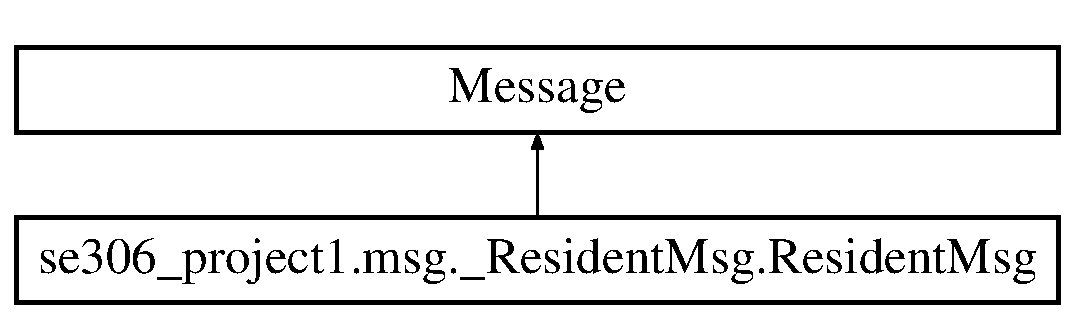
\includegraphics[height=2.000000cm]{classse306__project1_1_1msg_1_1__ResidentMsg_1_1ResidentMsg}
\end{center}
\end{figure}
\subsection*{Public Member Functions}
\begin{DoxyCompactItemize}
\item 
def \hyperlink{classse306__project1_1_1msg_1_1__ResidentMsg_1_1ResidentMsg_a478d608feb54103df63be92f56924b28}{\-\_\-\-\_\-init\-\_\-\-\_\-}
\item 
def \hyperlink{classse306__project1_1_1msg_1_1__ResidentMsg_1_1ResidentMsg_a8e5f5cd5b2bd07c32ed735978ffeb4ee}{serialize}
\item 
def \hyperlink{classse306__project1_1_1msg_1_1__ResidentMsg_1_1ResidentMsg_ac11744354ea648bc3df1aa92e8c799d7}{deserialize}
\item 
def \hyperlink{classse306__project1_1_1msg_1_1__ResidentMsg_1_1ResidentMsg_a86f69bc9eaa9d1b5c9ffdb581266e584}{serialize\-\_\-numpy}
\item 
def \hyperlink{classse306__project1_1_1msg_1_1__ResidentMsg_1_1ResidentMsg_a8608a64edc2229ed55f0669caf76153d}{deserialize\-\_\-numpy}
\end{DoxyCompactItemize}
\subsection*{Public Attributes}
\begin{DoxyCompactItemize}
\item 
\hypertarget{classse306__project1_1_1msg_1_1__ResidentMsg_1_1ResidentMsg_a8009f9a9bb29b41063fe71c6414086c2}{{\bfseries current\-Checkpoint\-X}}\label{classse306__project1_1_1msg_1_1__ResidentMsg_1_1ResidentMsg_a8009f9a9bb29b41063fe71c6414086c2}

\item 
\hypertarget{classse306__project1_1_1msg_1_1__ResidentMsg_1_1ResidentMsg_a805f3fd3378d0de178b46f4cbfc819ae}{{\bfseries current\-Checkpoint\-Y}}\label{classse306__project1_1_1msg_1_1__ResidentMsg_1_1ResidentMsg_a805f3fd3378d0de178b46f4cbfc819ae}

\item 
\hypertarget{classse306__project1_1_1msg_1_1__ResidentMsg_1_1ResidentMsg_a3b670ca0b10f87052536b9e55ad16d59}{{\bfseries state}}\label{classse306__project1_1_1msg_1_1__ResidentMsg_1_1ResidentMsg_a3b670ca0b10f87052536b9e55ad16d59}

\item 
\hypertarget{classse306__project1_1_1msg_1_1__ResidentMsg_1_1ResidentMsg_ab6b95718ade42ea15a777a23711884c8}{{\bfseries current\-Checkpoint}}\label{classse306__project1_1_1msg_1_1__ResidentMsg_1_1ResidentMsg_ab6b95718ade42ea15a777a23711884c8}

\end{DoxyCompactItemize}


\subsection{Constructor \& Destructor Documentation}
\hypertarget{classse306__project1_1_1msg_1_1__ResidentMsg_1_1ResidentMsg_a478d608feb54103df63be92f56924b28}{\index{se306\-\_\-project1\-::msg\-::\-\_\-\-Resident\-Msg\-::\-Resident\-Msg@{se306\-\_\-project1\-::msg\-::\-\_\-\-Resident\-Msg\-::\-Resident\-Msg}!\-\_\-\-\_\-init\-\_\-\-\_\-@{\-\_\-\-\_\-init\-\_\-\-\_\-}}
\index{\-\_\-\-\_\-init\-\_\-\-\_\-@{\-\_\-\-\_\-init\-\_\-\-\_\-}!se306_project1::msg::_ResidentMsg::ResidentMsg@{se306\-\_\-project1\-::msg\-::\-\_\-\-Resident\-Msg\-::\-Resident\-Msg}}
\subsubsection[{\-\_\-\-\_\-init\-\_\-\-\_\-}]{\setlength{\rightskip}{0pt plus 5cm}def se306\-\_\-project1.\-msg.\-\_\-\-Resident\-Msg.\-Resident\-Msg.\-\_\-\-\_\-init\-\_\-\-\_\- (
\begin{DoxyParamCaption}
\item[{}]{self, }
\item[{}]{args, }
\item[{}]{kwds}
\end{DoxyParamCaption}
)}}\label{classse306__project1_1_1msg_1_1__ResidentMsg_1_1ResidentMsg_a478d608feb54103df63be92f56924b28}
\begin{DoxyVerb}Constructor. Any message fields that are implicitly/explicitly
set to None will be assigned a default value. The recommend
use is keyword arguments as this is more robust to future message
changes.  You cannot mix in-order arguments and keyword arguments.

The available fields are:
   currentCheckpointX,currentCheckpointY,state,currentCheckpoint

:param args: complete set of field values, in .msg order
:param kwds: use keyword arguments corresponding to message field names
to set specific fields.
\end{DoxyVerb}
 

\subsection{Member Function Documentation}
\hypertarget{classse306__project1_1_1msg_1_1__ResidentMsg_1_1ResidentMsg_ac11744354ea648bc3df1aa92e8c799d7}{\index{se306\-\_\-project1\-::msg\-::\-\_\-\-Resident\-Msg\-::\-Resident\-Msg@{se306\-\_\-project1\-::msg\-::\-\_\-\-Resident\-Msg\-::\-Resident\-Msg}!deserialize@{deserialize}}
\index{deserialize@{deserialize}!se306_project1::msg::_ResidentMsg::ResidentMsg@{se306\-\_\-project1\-::msg\-::\-\_\-\-Resident\-Msg\-::\-Resident\-Msg}}
\subsubsection[{deserialize}]{\setlength{\rightskip}{0pt plus 5cm}def se306\-\_\-project1.\-msg.\-\_\-\-Resident\-Msg.\-Resident\-Msg.\-deserialize (
\begin{DoxyParamCaption}
\item[{}]{self, }
\item[{}]{str}
\end{DoxyParamCaption}
)}}\label{classse306__project1_1_1msg_1_1__ResidentMsg_1_1ResidentMsg_ac11744354ea648bc3df1aa92e8c799d7}
\begin{DoxyVerb}unpack serialized message in str into this message instance
:param str: byte array of serialized message, ``str``
\end{DoxyVerb}
 \hypertarget{classse306__project1_1_1msg_1_1__ResidentMsg_1_1ResidentMsg_a8608a64edc2229ed55f0669caf76153d}{\index{se306\-\_\-project1\-::msg\-::\-\_\-\-Resident\-Msg\-::\-Resident\-Msg@{se306\-\_\-project1\-::msg\-::\-\_\-\-Resident\-Msg\-::\-Resident\-Msg}!deserialize\-\_\-numpy@{deserialize\-\_\-numpy}}
\index{deserialize\-\_\-numpy@{deserialize\-\_\-numpy}!se306_project1::msg::_ResidentMsg::ResidentMsg@{se306\-\_\-project1\-::msg\-::\-\_\-\-Resident\-Msg\-::\-Resident\-Msg}}
\subsubsection[{deserialize\-\_\-numpy}]{\setlength{\rightskip}{0pt plus 5cm}def se306\-\_\-project1.\-msg.\-\_\-\-Resident\-Msg.\-Resident\-Msg.\-deserialize\-\_\-numpy (
\begin{DoxyParamCaption}
\item[{}]{self, }
\item[{}]{str, }
\item[{}]{numpy}
\end{DoxyParamCaption}
)}}\label{classse306__project1_1_1msg_1_1__ResidentMsg_1_1ResidentMsg_a8608a64edc2229ed55f0669caf76153d}
\begin{DoxyVerb}unpack serialized message in str into this message instance using numpy for array types
:param str: byte array of serialized message, ``str``
:param numpy: numpy python module
\end{DoxyVerb}
 \hypertarget{classse306__project1_1_1msg_1_1__ResidentMsg_1_1ResidentMsg_a8e5f5cd5b2bd07c32ed735978ffeb4ee}{\index{se306\-\_\-project1\-::msg\-::\-\_\-\-Resident\-Msg\-::\-Resident\-Msg@{se306\-\_\-project1\-::msg\-::\-\_\-\-Resident\-Msg\-::\-Resident\-Msg}!serialize@{serialize}}
\index{serialize@{serialize}!se306_project1::msg::_ResidentMsg::ResidentMsg@{se306\-\_\-project1\-::msg\-::\-\_\-\-Resident\-Msg\-::\-Resident\-Msg}}
\subsubsection[{serialize}]{\setlength{\rightskip}{0pt plus 5cm}def se306\-\_\-project1.\-msg.\-\_\-\-Resident\-Msg.\-Resident\-Msg.\-serialize (
\begin{DoxyParamCaption}
\item[{}]{self, }
\item[{}]{buff}
\end{DoxyParamCaption}
)}}\label{classse306__project1_1_1msg_1_1__ResidentMsg_1_1ResidentMsg_a8e5f5cd5b2bd07c32ed735978ffeb4ee}
\begin{DoxyVerb}serialize message into buffer
:param buff: buffer, ``StringIO``
\end{DoxyVerb}
 \hypertarget{classse306__project1_1_1msg_1_1__ResidentMsg_1_1ResidentMsg_a86f69bc9eaa9d1b5c9ffdb581266e584}{\index{se306\-\_\-project1\-::msg\-::\-\_\-\-Resident\-Msg\-::\-Resident\-Msg@{se306\-\_\-project1\-::msg\-::\-\_\-\-Resident\-Msg\-::\-Resident\-Msg}!serialize\-\_\-numpy@{serialize\-\_\-numpy}}
\index{serialize\-\_\-numpy@{serialize\-\_\-numpy}!se306_project1::msg::_ResidentMsg::ResidentMsg@{se306\-\_\-project1\-::msg\-::\-\_\-\-Resident\-Msg\-::\-Resident\-Msg}}
\subsubsection[{serialize\-\_\-numpy}]{\setlength{\rightskip}{0pt plus 5cm}def se306\-\_\-project1.\-msg.\-\_\-\-Resident\-Msg.\-Resident\-Msg.\-serialize\-\_\-numpy (
\begin{DoxyParamCaption}
\item[{}]{self, }
\item[{}]{buff, }
\item[{}]{numpy}
\end{DoxyParamCaption}
)}}\label{classse306__project1_1_1msg_1_1__ResidentMsg_1_1ResidentMsg_a86f69bc9eaa9d1b5c9ffdb581266e584}
\begin{DoxyVerb}serialize message with numpy array types into buffer
:param buff: buffer, ``StringIO``
:param numpy: numpy python module
\end{DoxyVerb}
 

The documentation for this class was generated from the following file\-:\begin{DoxyCompactItemize}
\item 
se306\-\_\-project1/src/se306\-\_\-project1/msg/\-\_\-\-Resident\-Msg.\-py\end{DoxyCompactItemize}

\hypertarget{structse306__project1_1_1ResidentMsg__}{\section{se306\-\_\-project1\-:\-:Resident\-Msg\-\_\-$<$ Container\-Allocator $>$ Struct Template Reference}
\label{structse306__project1_1_1ResidentMsg__}\index{se306\-\_\-project1\-::\-Resident\-Msg\-\_\-$<$ Container\-Allocator $>$@{se306\-\_\-project1\-::\-Resident\-Msg\-\_\-$<$ Container\-Allocator $>$}}
}
\subsection*{Public Types}
\begin{DoxyCompactItemize}
\item 
\hypertarget{structse306__project1_1_1ResidentMsg___a333e27c02fbdf82c901465a81a269879}{typedef \hyperlink{structse306__project1_1_1ResidentMsg__}{Resident\-Msg\-\_\-}\\*
$<$ Container\-Allocator $>$ {\bfseries Type}}\label{structse306__project1_1_1ResidentMsg___a333e27c02fbdf82c901465a81a269879}

\item 
\hypertarget{structse306__project1_1_1ResidentMsg___a6b445d2d307a6fd1fc69d568184ce3bc}{typedef double {\bfseries \-\_\-current\-Checkpoint\-X\-\_\-type}}\label{structse306__project1_1_1ResidentMsg___a6b445d2d307a6fd1fc69d568184ce3bc}

\item 
\hypertarget{structse306__project1_1_1ResidentMsg___a57cbeccc1d9a09e184648aad4cc33663}{typedef double {\bfseries \-\_\-current\-Checkpoint\-Y\-\_\-type}}\label{structse306__project1_1_1ResidentMsg___a57cbeccc1d9a09e184648aad4cc33663}

\item 
\hypertarget{structse306__project1_1_1ResidentMsg___a18975e7e3c2118a7e6a22711b7e609b1}{typedef std\-::basic\-\_\-string\\*
$<$ char, std\-::char\-\_\-traits$<$ char $>$\\*
, typename \\*
Container\-Allocator\-::template \\*
rebind$<$ char $>$\-::other $>$ {\bfseries \-\_\-state\-\_\-type}}\label{structse306__project1_1_1ResidentMsg___a18975e7e3c2118a7e6a22711b7e609b1}

\item 
\hypertarget{structse306__project1_1_1ResidentMsg___a9478e72b91b6e6a025430914d5ea923f}{typedef std\-::basic\-\_\-string\\*
$<$ char, std\-::char\-\_\-traits$<$ char $>$\\*
, typename \\*
Container\-Allocator\-::template \\*
rebind$<$ char $>$\-::other $>$ {\bfseries \-\_\-current\-Checkpoint\-\_\-type}}\label{structse306__project1_1_1ResidentMsg___a9478e72b91b6e6a025430914d5ea923f}

\item 
\hypertarget{structse306__project1_1_1ResidentMsg___ab2377a7f29370a11badbb8469ab8b811}{typedef boost\-::shared\-\_\-ptr\\*
$<$ \-::\hyperlink{structse306__project1_1_1ResidentMsg__}{se306\-\_\-project1\-::\-Resident\-Msg\-\_\-}\\*
$<$ Container\-Allocator $>$ $>$ {\bfseries Ptr}}\label{structse306__project1_1_1ResidentMsg___ab2377a7f29370a11badbb8469ab8b811}

\item 
\hypertarget{structse306__project1_1_1ResidentMsg___a303bbdaa992130e86797f04c3754c962}{typedef boost\-::shared\-\_\-ptr\\*
$<$ \-::\hyperlink{structse306__project1_1_1ResidentMsg__}{se306\-\_\-project1\-::\-Resident\-Msg\-\_\-}\\*
$<$ Container\-Allocator $>$ const  $>$ {\bfseries Const\-Ptr}}\label{structse306__project1_1_1ResidentMsg___a303bbdaa992130e86797f04c3754c962}

\end{DoxyCompactItemize}
\subsection*{Public Member Functions}
\begin{DoxyCompactItemize}
\item 
\hypertarget{structse306__project1_1_1ResidentMsg___acd6d23f75b6ac337376a428469ba11f3}{{\bfseries Resident\-Msg\-\_\-} (const Container\-Allocator \&\-\_\-alloc)}\label{structse306__project1_1_1ResidentMsg___acd6d23f75b6ac337376a428469ba11f3}

\end{DoxyCompactItemize}
\subsection*{Public Attributes}
\begin{DoxyCompactItemize}
\item 
\hypertarget{structse306__project1_1_1ResidentMsg___aad2a35f578c3ed9a1bc6b537163378ae}{double {\bfseries current\-Checkpoint\-X}}\label{structse306__project1_1_1ResidentMsg___aad2a35f578c3ed9a1bc6b537163378ae}

\item 
\hypertarget{structse306__project1_1_1ResidentMsg___afb1841a045e6bc072dc683414c3fdd1d}{double {\bfseries current\-Checkpoint\-Y}}\label{structse306__project1_1_1ResidentMsg___afb1841a045e6bc072dc683414c3fdd1d}

\item 
\hypertarget{structse306__project1_1_1ResidentMsg___a4035eb47fd7b516964e40cffb1dfe575}{std\-::basic\-\_\-string$<$ char, \\*
std\-::char\-\_\-traits$<$ char $>$\\*
, typename \\*
Container\-Allocator\-::template \\*
rebind$<$ char $>$\-::other $>$ {\bfseries state}}\label{structse306__project1_1_1ResidentMsg___a4035eb47fd7b516964e40cffb1dfe575}

\item 
\hypertarget{structse306__project1_1_1ResidentMsg___a82f6ec02330664d82be5bed971f6471e}{std\-::basic\-\_\-string$<$ char, \\*
std\-::char\-\_\-traits$<$ char $>$\\*
, typename \\*
Container\-Allocator\-::template \\*
rebind$<$ char $>$\-::other $>$ {\bfseries current\-Checkpoint}}\label{structse306__project1_1_1ResidentMsg___a82f6ec02330664d82be5bed971f6471e}

\end{DoxyCompactItemize}


The documentation for this struct was generated from the following file\-:\begin{DoxyCompactItemize}
\item 
se306\-\_\-project1/msg\-\_\-gen/cpp/include/se306\-\_\-project1/Resident\-Msg.\-h\end{DoxyCompactItemize}

\hypertarget{classrosGUI_1_1ros__gui}{\section{ros\-G\-U\-I.\-ros\-\_\-gui Class Reference}
\label{classrosGUI_1_1ros__gui}\index{ros\-G\-U\-I.\-ros\-\_\-gui@{ros\-G\-U\-I.\-ros\-\_\-gui}}
}
Inheritance diagram for ros\-G\-U\-I.\-ros\-\_\-gui\-:\begin{figure}[H]
\begin{center}
\leavevmode
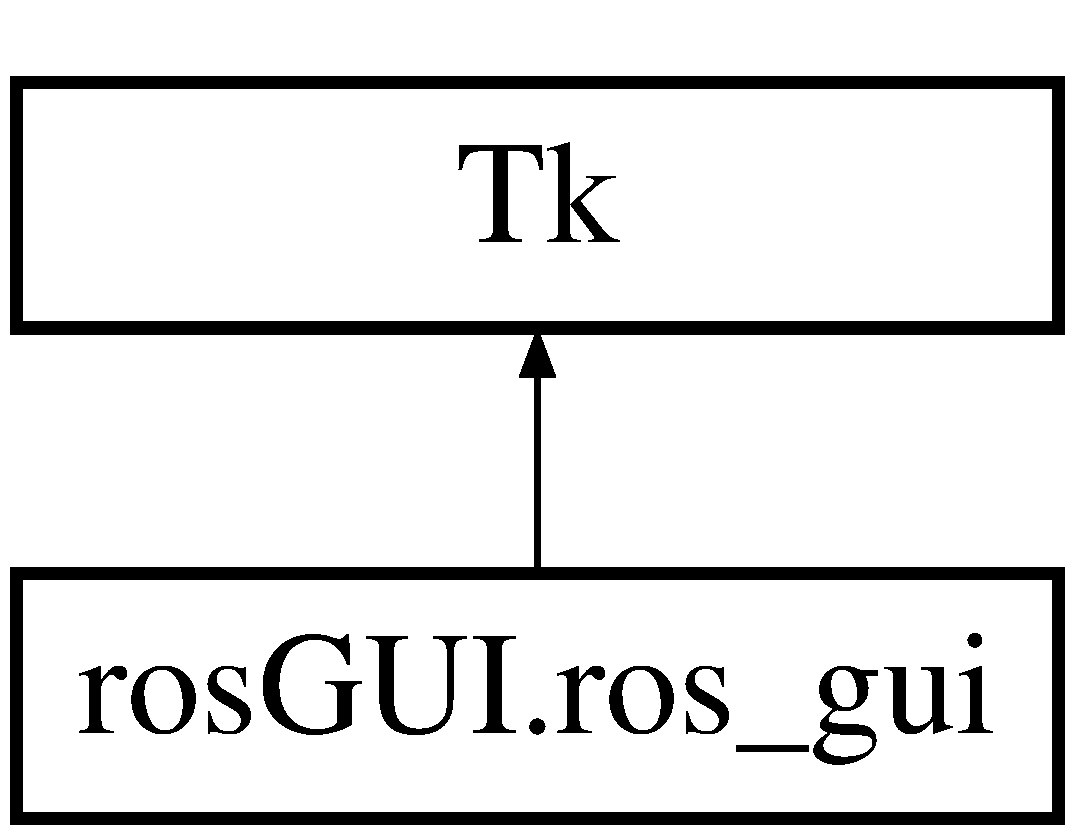
\includegraphics[height=2.000000cm]{classrosGUI_1_1ros__gui}
\end{center}
\end{figure}
\subsection*{Public Member Functions}
\begin{DoxyCompactItemize}
\item 
\hypertarget{classrosGUI_1_1ros__gui_ac3440f21602583cba395cdb3c6972199}{def {\bfseries \-\_\-\-\_\-init\-\_\-\-\_\-}}\label{classrosGUI_1_1ros__gui_ac3440f21602583cba395cdb3c6972199}

\item 
\hypertarget{classrosGUI_1_1ros__gui_a0ea7365b3064802a5439a8bece3f7c18}{def {\bfseries initialize}}\label{classrosGUI_1_1ros__gui_a0ea7365b3064802a5439a8bece3f7c18}

\item 
\hypertarget{classrosGUI_1_1ros__gui_af657d49b93f446b0a9b43a6f7161ab4c}{def {\bfseries setup\-Node}}\label{classrosGUI_1_1ros__gui_af657d49b93f446b0a9b43a6f7161ab4c}

\item 
\hypertarget{classrosGUI_1_1ros__gui_a5e1f672c68ef5d8bafe18b6e8f3e6edf}{def {\bfseries resident\-Status\-Callback}}\label{classrosGUI_1_1ros__gui_a5e1f672c68ef5d8bafe18b6e8f3e6edf}

\item 
\hypertarget{classrosGUI_1_1ros__gui_ac388ca6fe6783f826844da976d513442}{def {\bfseries decrease\-Health}}\label{classrosGUI_1_1ros__gui_ac388ca6fe6783f826844da976d513442}

\end{DoxyCompactItemize}
\subsection*{Public Attributes}
\begin{DoxyCompactItemize}
\item 
\hypertarget{classrosGUI_1_1ros__gui_ac0f9ef4869c1ab2000e84e6cb561709d}{{\bfseries parent}}\label{classrosGUI_1_1ros__gui_ac0f9ef4869c1ab2000e84e6cb561709d}

\item 
\hypertarget{classrosGUI_1_1ros__gui_a0b33da1d02d080ce67d5299168068044}{{\bfseries health\-Bar}}\label{classrosGUI_1_1ros__gui_a0b33da1d02d080ce67d5299168068044}

\item 
\hypertarget{classrosGUI_1_1ros__gui_a0c0e884fb3adf543064604a43a0920c2}{{\bfseries health\-Filler}}\label{classrosGUI_1_1ros__gui_a0c0e884fb3adf543064604a43a0920c2}

\item 
\hypertarget{classrosGUI_1_1ros__gui_a528931d908c4d72c307bf1f559efac5a}{{\bfseries hunger\-Bar}}\label{classrosGUI_1_1ros__gui_a528931d908c4d72c307bf1f559efac5a}

\item 
\hypertarget{classrosGUI_1_1ros__gui_a20aa4aff7210fbe8a4c5a12beb86d1ee}{{\bfseries hunger\-Filler}}\label{classrosGUI_1_1ros__gui_a20aa4aff7210fbe8a4c5a12beb86d1ee}

\item 
\hypertarget{classrosGUI_1_1ros__gui_af2662950f1e429e25656ad60db742199}{{\bfseries boredom\-Bar}}\label{classrosGUI_1_1ros__gui_af2662950f1e429e25656ad60db742199}

\item 
\hypertarget{classrosGUI_1_1ros__gui_a810b52b8e2c517efab7b8b0d1796dbaf}{{\bfseries boredom\-Filler}}\label{classrosGUI_1_1ros__gui_a810b52b8e2c517efab7b8b0d1796dbaf}

\item 
\hypertarget{classrosGUI_1_1ros__gui_a1150c1d22b7c1e48bbdd53d339beb0b8}{{\bfseries pos\-Val}}\label{classrosGUI_1_1ros__gui_a1150c1d22b7c1e48bbdd53d339beb0b8}

\item 
\hypertarget{classrosGUI_1_1ros__gui_af6bcd76c1a8d35589c3c4336d822cb5d}{{\bfseries state\-Resident}}\label{classrosGUI_1_1ros__gui_af6bcd76c1a8d35589c3c4336d822cb5d}

\end{DoxyCompactItemize}


The documentation for this class was generated from the following file\-:\begin{DoxyCompactItemize}
\item 
se306\-\_\-project1/src/ros\-G\-U\-I.\-py\end{DoxyCompactItemize}

\hypertarget{structros_1_1serialization_1_1Serializer_3_01_1_1se306__project1_1_1AssistantMsg___3_01ContainerAllocator_01_4_01_4}{\section{ros\-:\-:serialization\-:\-:Serializer$<$ \-:\-:se306\-\_\-project1\-:\-:Assistant\-Msg\-\_\-$<$ Container\-Allocator $>$ $>$ Struct Template Reference}
\label{structros_1_1serialization_1_1Serializer_3_01_1_1se306__project1_1_1AssistantMsg___3_01ContainerAllocator_01_4_01_4}\index{ros\-::serialization\-::\-Serializer$<$ \-::se306\-\_\-project1\-::\-Assistant\-Msg\-\_\-$<$ Container\-Allocator $>$ $>$@{ros\-::serialization\-::\-Serializer$<$ \-::se306\-\_\-project1\-::\-Assistant\-Msg\-\_\-$<$ Container\-Allocator $>$ $>$}}
}
\subsection*{Static Public Member Functions}
\begin{DoxyCompactItemize}
\item 
\hypertarget{structros_1_1serialization_1_1Serializer_3_01_1_1se306__project1_1_1AssistantMsg___3_01ContainerAllocator_01_4_01_4_a58727bd9bc3275aef940137c5dbb8cb4}{{\footnotesize template$<$typename Stream , typename T $>$ }\\static void {\bfseries all\-In\-One} (Stream \&stream, T m)}\label{structros_1_1serialization_1_1Serializer_3_01_1_1se306__project1_1_1AssistantMsg___3_01ContainerAllocator_01_4_01_4_a58727bd9bc3275aef940137c5dbb8cb4}

\end{DoxyCompactItemize}
\subsection*{Public Attributes}
\begin{DoxyCompactItemize}
\item 
\hypertarget{structros_1_1serialization_1_1Serializer_3_01_1_1se306__project1_1_1AssistantMsg___3_01ContainerAllocator_01_4_01_4_a93a5cd662051d08aa1cd89b6b7763aba}{{\bfseries R\-O\-S\-\_\-\-D\-E\-C\-L\-A\-R\-E\-\_\-\-A\-L\-L\-I\-N\-O\-N\-E\-\_\-\-S\-E\-R\-I\-A\-L\-I\-Z\-E\-R}}\label{structros_1_1serialization_1_1Serializer_3_01_1_1se306__project1_1_1AssistantMsg___3_01ContainerAllocator_01_4_01_4_a93a5cd662051d08aa1cd89b6b7763aba}

\end{DoxyCompactItemize}


The documentation for this struct was generated from the following file\-:\begin{DoxyCompactItemize}
\item 
se306\-\_\-project1/msg\-\_\-gen/cpp/include/se306\-\_\-project1/Assistant\-Msg.\-h\end{DoxyCompactItemize}

\hypertarget{structros_1_1serialization_1_1Serializer_3_01_1_1se306__project1_1_1DoctorMsg___3_01ContainerAllocator_01_4_01_4}{\section{ros\-:\-:serialization\-:\-:Serializer$<$ \-:\-:se306\-\_\-project1\-:\-:Doctor\-Msg\-\_\-$<$ Container\-Allocator $>$ $>$ Struct Template Reference}
\label{structros_1_1serialization_1_1Serializer_3_01_1_1se306__project1_1_1DoctorMsg___3_01ContainerAllocator_01_4_01_4}\index{ros\-::serialization\-::\-Serializer$<$ \-::se306\-\_\-project1\-::\-Doctor\-Msg\-\_\-$<$ Container\-Allocator $>$ $>$@{ros\-::serialization\-::\-Serializer$<$ \-::se306\-\_\-project1\-::\-Doctor\-Msg\-\_\-$<$ Container\-Allocator $>$ $>$}}
}
\subsection*{Static Public Member Functions}
\begin{DoxyCompactItemize}
\item 
\hypertarget{structros_1_1serialization_1_1Serializer_3_01_1_1se306__project1_1_1DoctorMsg___3_01ContainerAllocator_01_4_01_4_a71aa8b9037f829dfb99270b70becea54}{{\footnotesize template$<$typename Stream , typename T $>$ }\\static void {\bfseries all\-In\-One} (Stream \&stream, T m)}\label{structros_1_1serialization_1_1Serializer_3_01_1_1se306__project1_1_1DoctorMsg___3_01ContainerAllocator_01_4_01_4_a71aa8b9037f829dfb99270b70becea54}

\end{DoxyCompactItemize}
\subsection*{Public Attributes}
\begin{DoxyCompactItemize}
\item 
\hypertarget{structros_1_1serialization_1_1Serializer_3_01_1_1se306__project1_1_1DoctorMsg___3_01ContainerAllocator_01_4_01_4_a6ce4bfe803f9d9939193782f674e5c37}{{\bfseries R\-O\-S\-\_\-\-D\-E\-C\-L\-A\-R\-E\-\_\-\-A\-L\-L\-I\-N\-O\-N\-E\-\_\-\-S\-E\-R\-I\-A\-L\-I\-Z\-E\-R}}\label{structros_1_1serialization_1_1Serializer_3_01_1_1se306__project1_1_1DoctorMsg___3_01ContainerAllocator_01_4_01_4_a6ce4bfe803f9d9939193782f674e5c37}

\end{DoxyCompactItemize}


The documentation for this struct was generated from the following file\-:\begin{DoxyCompactItemize}
\item 
se306\-\_\-project1/msg\-\_\-gen/cpp/include/se306\-\_\-project1/Doctor\-Msg.\-h\end{DoxyCompactItemize}

\hypertarget{structros_1_1serialization_1_1Serializer_3_01_1_1se306__project1_1_1ResidentMsg___3_01ContainerAllocator_01_4_01_4}{\section{ros\-:\-:serialization\-:\-:Serializer$<$ \-:\-:se306\-\_\-project1\-:\-:Resident\-Msg\-\_\-$<$ Container\-Allocator $>$ $>$ Struct Template Reference}
\label{structros_1_1serialization_1_1Serializer_3_01_1_1se306__project1_1_1ResidentMsg___3_01ContainerAllocator_01_4_01_4}\index{ros\-::serialization\-::\-Serializer$<$ \-::se306\-\_\-project1\-::\-Resident\-Msg\-\_\-$<$ Container\-Allocator $>$ $>$@{ros\-::serialization\-::\-Serializer$<$ \-::se306\-\_\-project1\-::\-Resident\-Msg\-\_\-$<$ Container\-Allocator $>$ $>$}}
}
\subsection*{Static Public Member Functions}
\begin{DoxyCompactItemize}
\item 
\hypertarget{structros_1_1serialization_1_1Serializer_3_01_1_1se306__project1_1_1ResidentMsg___3_01ContainerAllocator_01_4_01_4_ad3478d0ec2e0f6c8818c4435fdedf979}{{\footnotesize template$<$typename Stream , typename T $>$ }\\static void {\bfseries all\-In\-One} (Stream \&stream, T m)}\label{structros_1_1serialization_1_1Serializer_3_01_1_1se306__project1_1_1ResidentMsg___3_01ContainerAllocator_01_4_01_4_ad3478d0ec2e0f6c8818c4435fdedf979}

\end{DoxyCompactItemize}
\subsection*{Public Attributes}
\begin{DoxyCompactItemize}
\item 
\hypertarget{structros_1_1serialization_1_1Serializer_3_01_1_1se306__project1_1_1ResidentMsg___3_01ContainerAllocator_01_4_01_4_a831a379812e81672e65c4689dc390c88}{{\bfseries R\-O\-S\-\_\-\-D\-E\-C\-L\-A\-R\-E\-\_\-\-A\-L\-L\-I\-N\-O\-N\-E\-\_\-\-S\-E\-R\-I\-A\-L\-I\-Z\-E\-R}}\label{structros_1_1serialization_1_1Serializer_3_01_1_1se306__project1_1_1ResidentMsg___3_01ContainerAllocator_01_4_01_4_a831a379812e81672e65c4689dc390c88}

\end{DoxyCompactItemize}


The documentation for this struct was generated from the following file\-:\begin{DoxyCompactItemize}
\item 
se306\-\_\-project1/msg\-\_\-gen/cpp/include/se306\-\_\-project1/Resident\-Msg.\-h\end{DoxyCompactItemize}

\hypertarget{structstatusObj}{\section{status\-Obj Struct Reference}
\label{structstatusObj}\index{status\-Obj@{status\-Obj}}
}
\subsection*{Public Attributes}
\begin{DoxyCompactItemize}
\item 
\hypertarget{structstatusObj_a133b14a8f17b2b31d52ecf6ef6a8fe6e}{int {\bfseries priority}}\label{structstatusObj_a133b14a8f17b2b31d52ecf6ef6a8fe6e}

\item 
\hypertarget{structstatusObj_a65ed97f7deaf094ed3640b26a3527588}{resident\-States {\bfseries state}}\label{structstatusObj_a65ed97f7deaf094ed3640b26a3527588}

\end{DoxyCompactItemize}


The documentation for this struct was generated from the following file\-:\begin{DoxyCompactItemize}
\item 
se306\-\_\-project1/src/priority\-Queue.\-cpp\end{DoxyCompactItemize}

\hypertarget{classVisitor}{\section{Visitor Class Reference}
\label{classVisitor}\index{Visitor@{Visitor}}
}


Class for the implementation of visitors -\/ i.\-e. Caregivers, Nurses, Doctors, Friends, and Relatives.  




{\ttfamily \#include $<$Visitor.\-h$>$}

Inheritance diagram for Visitor\-:\begin{figure}[H]
\begin{center}
\leavevmode
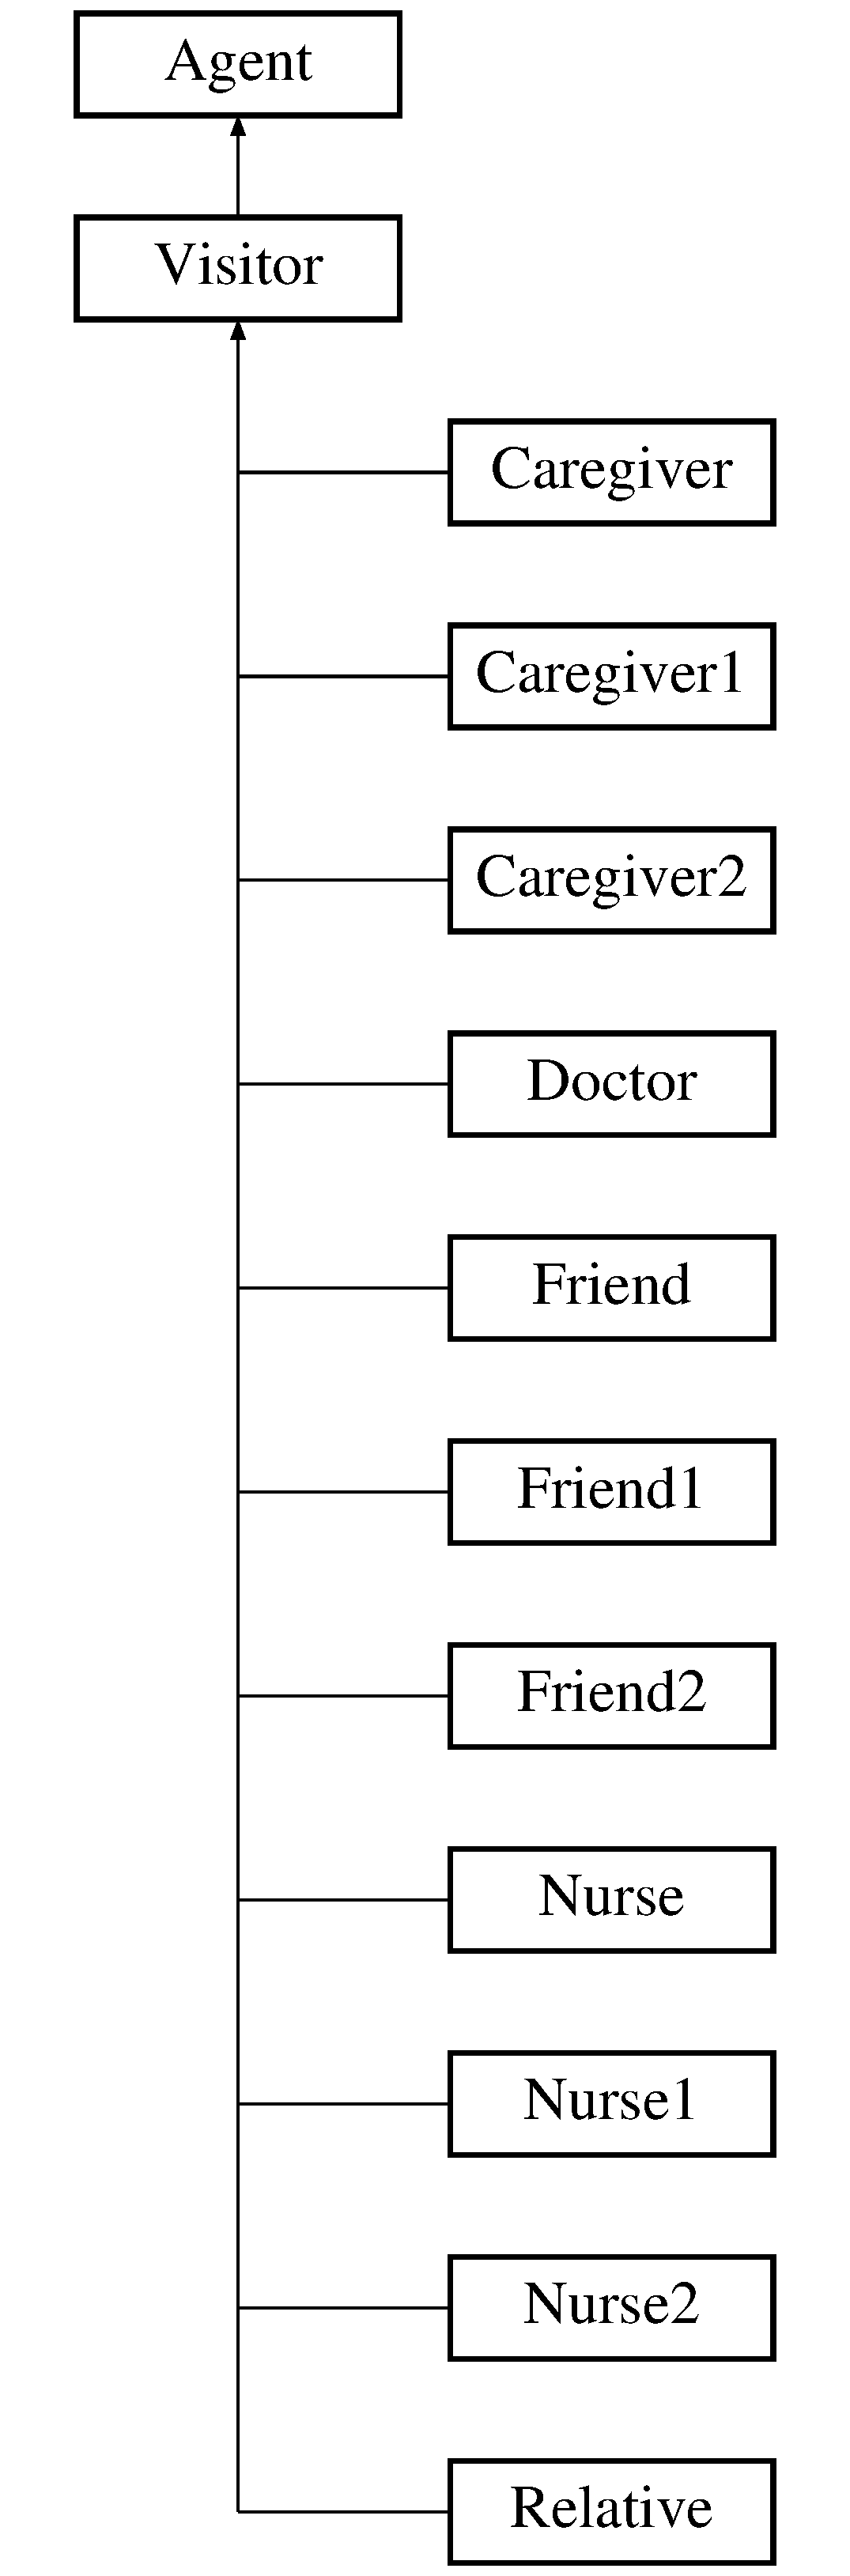
\includegraphics[height=3.000000cm]{classVisitor}
\end{center}
\end{figure}
\subsection*{Additional Inherited Members}


\subsection{Detailed Description}
Class for the implementation of visitors -\/ i.\-e. Caregivers, Nurses, Doctors, Friends, and Relatives. 

The documentation for this class was generated from the following file\-:\begin{DoxyCompactItemize}
\item 
se306\-\_\-project1/src/Visitor.\-h\end{DoxyCompactItemize}

%--- End generated contents ---

% Index
\newpage
\phantomsection
\addcontentsline{toc}{chapter}{Index}
\printindex

\end{document}
